\chapter{Thermodynamic modeling of fluoride and chloride molten salts with model selection, uncertainty quantification, and uncertainty propagation} \label{chap:moltensalts}

\section{Introduction} \label{moltensalts:sec:intro}
Chromium (Cr) is one of the key elements in current reference structural materials for fluoride salt reactors, for example, the Hastelloy-N as the container material (72\%Ni-16\%Mo-7\%Cr-5\%Fe in wt.\%) \cite{koger1972evaluation, manly1958metallurgical}. In the fluoride salt environment, Cr in Ni-based alloy is more susceptible to corrosion compared to other metal elements \cite{olson2009materials, ouyang2014long, liu2020corrosion}. For example, Olson et al. \cite{olson2009materials} performed corrosion tests on a number of Ni-based alloys with different Cr alloying contents. They showed the dissolution of Cr into molten salt and correlated the relationship between Cr content and corrosion resistance \cite{olson2009materials}. Ouyang et al. \cite{ouyang2014long} investigated the corrosion behavior of Hastelloy-N in FLiNaK after 100-1000 h at 700 $^o$C, and the aggregate dissolution of Cr was observed. Recently, Liu et al. \cite{liu2020corrosion} studied Hastelloy-N and showed that the corrosion rate of Cr in FLiNaK-CrF$_3$ is higher than that in FLiBe-CrF$_3$ with Cr$^{3+}$ as the product. Thus, it is important to investigate solubility and multivariate distribution patterns of Cr in FLiNaK. The LiF-NaF-KF system has been extensively studied by many researchers in terms of modeling. Chartrand and Pelton \cite{chartrand2001thermodynamic}, Wang et al. \cite{wang2014phase}, and Ard et al. (MSTDB-TC database) \cite{ard2022development} have investigated this system through CALPHAD modeling. However, we noticed that thermodynamic modeling of the FLiNaK-CrF$_3$ system has been performed based on incomplete and empirically estimated thermochemical data by Yin et al. \cite{yin2018thermodynamic, yin2015thermodynamic} and Dumaire et al. \cite{dumaire2021thermodynamic}. A comprehensive study on the thermodynamic properties of all solid and liquid phases in the FLiNaK-CrF$_3$ system is yet to be conducted.

Chloride molten salts have gained significant attention for their potential applications in advanced nuclear reactors and pyroprocessing techniques \cite{sridharan2012thermal, mourogov2006potentialities, iizuka1997actinides}. Effective separation of fission products, such as lanthanides using pyroprocessing techniques, requires a comprehensive understanding of the thermodynamic properties of molten salts. The CALPHAD  modeling approach \cite{liu2020computational, lukas2007computational} is effective in investigating phase equilibrium and thermodynamic properties in multicomponent systems. For the modeling of complex molten salts, various thermodynamic models within the CALPHAD framework have been developed to capture intricate behaviors such as short-range ordering, including the associate model, two-sublattice ionic model, and MQMQA (see Section \ref{method:ssec:liqmodels}). However, systematically comparing these models and selecting the most appropriate model for molten salts remain a challenge due to different physical interpretations and the complexities involved in quantifying model performance.

In the present work, the fluoride system (LiF, NaF, KF, CrF${_2}$)-CrF${_3}$ and the chloride system LiCl-KCl-LaCl${_3}$ are modeled using the CALPHAD method, supplemented with thermochemical data by first-principles calculations. The open-source software tools of ESPEI \cite{bocklund2019espei} and PyCalphad \cite{otis2017pycalphad} were employed for the modeling process, which facilitates Bayesian parameter estimation, UQ, and Bayesian model selection in modeling molten salts. The present work compares thermodynamic models commonly used in CALPHAD modeling for liquid, providing insights into an effective model selection strategy. 

\section{Revisiting thermodynamics in (LiF, NaF, KF, CrF${_2}$)-CrF${_3}$ by first-principles calculations and CALPHAD modeling} \label{moltensalts:sec:FLiNaKCr}
The thermodynamic description of the (LiF, NaF, KF, CrF$_2$)-CrF$_3$ systems has been revisited, aiming for a better understanding of the effects of Cr on the FLiNaK molten salt. First-principles calculations based on DFT were performed to determine the electronic and structural properties of each compound, including the formation enthalpy, volume, and bulk modulus. DFT-based phonon calculations were carried out to determine the thermodynamic properties of compounds, for example, enthalpy, entropy, and heat capacity as functions of temperature. Phonon-based thermodynamic properties show a good agreement with experimental data of binary compounds LiF, NaF, KF, CrF$_3$, and CrF$_2$, establishing a solid foundation to determine thermodynamic properties of ternary compounds as well as to verify results estimated by the Neumann-Kopp rule. Additionally, DFT-based AIMD simulations were employed to predict the mixing enthalpies of liquid salts. Using DFT-based results and experimental data in the literature, the (LiF, NaF, KF, CrF$_2$)-CrF$_3$ system has been remodeled in terms of the CALPHAD approach using the MQMQA for liquid. Calculated phase stability in the present work shows an excellent agreement with experiments, indicating the effectiveness of combining DFT-based total energy, phonon, and AIMD calculations, and CALPHAD modeling to provide the thermodynamic description in complex molten salt systems.

\subsection{Modeling details} \label{moltensalts:ssec:FLiNaKCrmodel}
%%% Compounds information
The (LiF, NaF, KF, CrF$_2$)-CrF$_3$ system includes five binary (endmember) compounds, i.e., LiF, NaF, KF, CrF$_3$ and CrF$_2$, and eight ternary (intermetallic) compounds, i.e., Li$_3$CrF$_6$, Na$_3$CrF$_6$, Na$_5$Cr$_3$F$_{14}$, NaCrF$_4$, K$_3$CrF$_6$, K$_2$CrF$_5$, KCrF$_4$, and K$_2$Cr$_5$F$_{17}$. De Kozak first suggested these ternary compounds \cite{DeKozak1969} and confirmed by structural studies \cite{de1975systeme,miranday1975croissance, sturm1962phase, garcia2014electrostatic, brunton1969crystal, le2003distorted, manaka2011effects, sassoye2006crystal} via the X-ray diffraction (XRD) method, which was summarized by Dumaire et al. \cite{dumaire2021thermodynamic}. However, thermochemical data on these compounds is scarce. Yin et al. \cite{yin2018thermodynamic, yin2015thermodynamic, yin2014thermodynamic} performed DFT calculations at 0 K to determine the formation enthalpies of Li$_3$CrF$_6$, Na$_3$CrF$_6$, Na$_5$Cr$_3$F$_{14}$, NaCrF$_4$, and KCrF$_4$. Dumaire et al. \cite{dumaire2021thermodynamic} estimated the heat capacities of these compounds based on the Neumann-Kopp rule in terms of the compositional average of heat capacity values of the corresponding compounds or elements \cite{leitner2010application}. 

%%% Modeling and First-principles details for compounds
The present work treats the compounds and endmembers in the AF-CrF${_3}$ (A=Li, Na, and K) systems as stoichiometric compounds. Thermodynamic functions of the binary endmembers are taken from the JRC database \cite{konings2020comprehensive}, JANAF tables \cite{chase1982janaf}, IVTAN tables \cite{gurvich1993ivtanthermo}, and SSUB database \cite{sgteurl}. The Gibbs energy can be expressed as 
\begin{equation} \label{ms:eq:Gstoi}
    G_m=\Delta_f H_m^0 (298.15)-T S_m^0 (298.15)+\int_{298.15}^T C_{P,m} dT - T\int_{298.15}^T \dfrac{C_{P,m}}{T} dT
\end{equation}
where $\Delta_f H_m^0 (298.15)$ is the standard formation enthalpy, $S_m^0 (298.15)$ the standard entropy at 298.15 K, and $C_{P,m}$ the heat capacity. The thermodynamic data of ternary compounds, including enthalpy, entropy, and heat capacity are obtained through DFT-based first-principles and phonon calculations (see Section \ref{method:sec:firstprinciples}).

All DFT-based first-principles and phonon calculations in the present work were performed by the VASP \cite{kresse1996efficient} using the open-source software DFTTK \cite{wang2021dfttk}. The projector augmented-wave method (PAW) was used for electron-ion interactions to increase computational efficiency compared with the full potential methods \cite{blochl1994projector, kresse1999ultrasoft}. Electron exchange and correlation effects were described using both the local density approximation (LDA) \cite{perdew1981self} and the GGA \cite{perdew1996generalized}. In addition, the DFT+U approach was employed for 11 compounds containing Cr, i.e., CrF${_2}$, CrF${_3}$, Cr$_2$F$_5$, Li$_3$CrF$_6$, Na$_3$CrF$_6$, Na$_5$Cr$_3$F$_{14}$, NaCrF$_4$, K$_3$CrF$_6$, K$_2$CrF$_5$, KCrF$_4$, K$_2$Cr$_5$F$_{17}$. The effective U values for Cr were selected as 3.7 eV, considering 3$-$4eV was commonly used in the literature \cite{shi2009magnetism, mattsson2019density, huang2022dft}. The spin configurations were also considered for these 11 compounds containing Cr. All possible configurations by varying spin up and spin down of Cr atoms were explored by the ATAT code \cite{van2009multicomponent}. The spin configuration with the lowest energy for each Cr-containing compound was used for DFT and phonon calculations. Using DFTTK, structure information is the only required input, then robust relaxation schemes can be automatically performed to obtain equilibrium results at 0 K and thermodynamic properties at finite temperatures through the QHA. During DFTTK calculations, the plane-wave cutoff energy was set as 520 eV. Table \ref{ms:tab:DFTdetails} lists the k-points meshes for DFT-based total energy calculations, the supercell sizes and the k-points meshes for phonon calculations. The phonon DOS was analyzed using the YPHON code \cite{wang2014yphon}, which has been integrated into DFTTK \cite{wang2021dfttk}. 

%%% CALPHAD modeling details
The MQMQA \cite{pelton2001modified} is used to describe the liquid phase by considering the short-range ordering (SRO) that occurs in liquid salts. Here, the model (A, Cr)(F) is introduced and hence the A$_2$F$_2$, Cr$_2$F$_2$, and ACrF$_2$ quadruplets (A=Li, Na, and K) are formed to consider the interactions among them. Coordination numbers Z describe the SNN coordination number of the species $i$ (= Li, Na, K, Cr, or F) in quadruplets. Z of anions can be calculated to maintain charge neutrality as follows:
\begin{equation} \label{ms:eq:MQMZ}
    \dfrac{q_A}{(Z_{AB:FF}^A)}+\dfrac{q_B}{(Z_{AB:FF}^B)}=2\times \dfrac{q_F}{(Z_{AB:FF}^F)}
\end{equation}
where $q_i$ is the charges of ion $i$ (= Li, Na, K, Cr, or F). Table \ref{ms:tab:CrZ} shows the coordination numbers used in the present work.

\begin{table}[H]
    \centering
    \caption{Details of DFT-based first-principles calculations for each compound or phase, including space group, total atoms in the supercells, k-point meshes for structure relaxations, and the final static calculations (indicated by DFT), supercell sizes for phonon calculations, k-point meshes for phonon calculations.}
    \begin{tabular}{>{\raggedright\arraybackslash}m{2.5cm}>{\raggedright\arraybackslash}m{2cm}>{\raggedright\arraybackslash}m{2.5cm}>{\raggedright\arraybackslash}m{2.5cm}>{\raggedright\arraybackslash}m{2.8cm}>{\raggedright\arraybackslash}m{2.5cm}}
    \hline
     \textbf{Phase}&\textbf{Space group}&\textbf{Atoms in crystallographic cell}&\textbf{k-points for DFT}&\textbf{Atoms in supercell for phonon}&\textbf{k-points for phonon}\\
    \hline
        LiF&$Fm\Bar{3}m$&8&$10\times10\times10$&32&$10\times10\times10$\\
        NaF&$Fm\Bar{3}m$&8&$10\times10\times10$&32&$10\times10\times10$\\
        KF&$Fm\Bar{3}m$&8&$10\times10\times10$&32&$10\times10\times10$\\
        CrF${_3}$&$R\Bar{3}c$&24&$9\times9\times3$&24&$9\times9\times3$\\
        CrF${_2}$&$P2_1/c$&6&$14\times10\times9$&24&$13\times10\times9$\\
        Li$_3$CrF$_6$&$C2/c$&60&$2\times2\times2$&60&$2\times2\times2$\\
        Na$_3$CrF$_6$&$P2_1/c$&20&$9\times8\times5$&40&$9\times8\times5$\\
        Na$_5$Cr$_3$F$_{14}$&$P2_1/c$&44&$6\times6\times3$&44&$6\times6\times3$\\
        NaCrF$_4$&$P2_1/c$&24&$6\times8\times5$&24&$6\times8\times6$\\
        K$_3$CrF$_6$&$Fm\Bar{3}m$&40&$5\times5\times5$&40&$5\times5\times5$\\
        K$_2$CrF$_5$&$Pbcn$&128&$3\times1\times1$&128&$3\times1\times1$\\
        KCrF$_4$&$Pnma$&144&$3\times1\times1$&144&$3\times1\times1$\\
        K$_2$Cr$_5$F$_{17}$&$Cmcm$&96&$2\times2\times2$&96&$2\times2\times2$\\
        Cr$_2$F$_5$&$C2/c$&28&$6\times6\times6$&N/A&N/A\\
    \hline
    \end{tabular}
    \label{ms:tab:DFTdetails}
\end{table}

\begin{table}[H]
    \centering
    \caption{Coordination number used in the present CALPHAD modeling work with MQMQA for the liquid phase.}
    \begin{tabular}{>{\raggedright\arraybackslash}m{2.5cm}>{\raggedright\arraybackslash}m{2.5cm}>{\raggedright\arraybackslash}m{2.5cm}>{\raggedright\arraybackslash}m{2.5cm}>{\raggedright\arraybackslash}m{2.5cm}}
    \hline
    \textbf{A}&\textbf{B}&\textbf{$Z_{AB:FF}^A$}&\textbf{$Z_{AB:FF}^B$}&\textbf{$Z_{AB:FF}^F$}\\
    \hline
    Li$^+$&Li$^+$&6&6&6 \\
    Na$^+$&Na$^+$&6&6&6\\
    K$^+$&K$^+$&6&6&6\\
    Cr$^{3+}$&Cr$^{3+}$&6&6&2\\
    Li$^+$&Cr$^{3+}$&2&6&2\\
    Na$^+$&Cr$^{3+}$&4&6&2.7\\
    K$^+$&Cr$^{3+}$&6&6&3\\
    Cr$^{2+}$&Cr$^{3+}$&6&6&2.4\\
    Cr$^{2+}$&Cr$^{2+}$&6&6&3\\
    \hline
    \end{tabular}
    \label{ms:tab:CrZ}
\end{table}

The excess Gibbs energy $G^{excess}$ relates to the formation Gibbs energy of the quadruplet, $\Delta g_{quadruplet}^{ex}$, by considering the following reaction:
\begin{equation} \label{ms:eq:MQMGrea}
    \left(\rm {A_2F_2}\right)_{quad}+\left({\rm Cr_2F_2}\right)_{quad}=2\left({\rm ACrF_2}\right)_{quad}\;\;\;\;\;\Delta g_{\rm ACr:F_2}^{ex}
\end{equation}
where $\Delta g_{\rm ACr:F_2}^{ex}$ represents the Gibbs energy change when forming the quadruplet and can be described by:
\begin{equation} \label{ms:eq:MQMGex}
    \Delta g_{\rm {ACr:F_2}}^{ex}=\Delta g_{\rm {ACr:F_2}}^o+\sum_{(i+j)\geq1} g_{\rm {ACr:F_2}}^{ij}\chi _{\rm {ACr:F_2}}^{i}\chi _{\rm {CrA:F_2}}^{j}
\end{equation}
where $g_{\rm {ACr:F_2}}^{ij}$ is a function of temperature and it is independent of composition. $\chi _{\rm {ACr:F_2}}^{i}$ and $\chi _{\rm {CrA:F_2}}^{j}$ are composition-dependent terms as:
\begin{equation} \label{ms:eq:chi}
    \chi_{\rm {ACr:F_2}} = \dfrac{X_{\rm {A_2:F_2}}}{X_{\rm {A_2:F_2}}+X_{\rm {ACr:F_2}}+X_{\rm {Cr_2:F_2}}}
\end{equation}
where $X_{\rm{ACr:F_2}}$ is the fractions of $\left(\rm{ACr:F_2}\right)_{quad}$ shown in (\ref{ms:eq:MQMGrea}). 

In the CrF${_2}$-CrF${_3}$ system, there are three solid solution phases, i.e., CrF${_2}$ near the Cr-rich region, CrF${_3}$ near the F-rich region, and Cr$_2$F$_5$ showing on the middle region of the CrF${_2}$-CrF${_3}$ phase diagram. The present work adopts the same models used by Dumaire et al. \cite{dumaire2021thermodynamic}, where the regular solution model with the Kohler-Toop interpolation \cite{kohler1960estimation, toop1965predicting, chartrand2000choice, pelton2001general} is used for Cr$_2$F$_5$. For solid solution phases near CrF${_2}$ and CrF${_3}$, the sublattice model is used for each phase, respectively, considering the Wyckoff positions of CrF${_2}$ and CrF${_3}$ as follows. CrF${_2}$ possesses the symmetry with space group $P2_1/c$ with two Wyckoff sites of 2a and 4e, and the sublattice model (Cr, Va)$_1$(F, Va)$_2$ is hence used with Va representing the vacancy. CrF${_3}$ phase is modeled by (Cr, Va)$_1$(F, Va)$_3$ by considering its space group $R\bar{3}c$ and the two Wyckoff sites of 2b and 6e. The Gibbs energy is formulated as:
\begin{equation} \label{ms:eq:Crssoln}
    \begin{aligned}
        G_m&=\sum_{i=Cr,Va}{\sum_{j=F,Va}{y_i^\prime y_j^{\prime\prime}}\:^oG_{i:j}}\\
        &+RT\left(\sum_{i=Cr,Va}{y_i^\prime\ln{\left(y_i^\prime\right)}}+\sum_{j=F,Va}{y_j^{\prime\prime}\ln{\left(y_j^{\prime\prime}\right)}}\right)\\&+y_{Cr}^\prime y_{Va}^\prime\left(y_F^{\prime\prime}L_{Cr,Va:F}\right)+y_F^{\prime\prime}y_{Va}^{\prime\prime}\left(y_{Cr}^\prime L_{Cr:F,Va}\right)
    \end{aligned}
\end{equation}
where $y_i^{(s)}$ is the site fraction of component i on sublattice s, ${^o}G_{i:j}$ the Gibbs energy of the endmember (i:j), and $L$ the interaction parameters which can be expanded using the Redlich-Kister polynomials \cite{redlich1948algebraic}. 

Phase equilibria in the LiF-CrF${_3}$, NaF-CrF${_3}$, and KF-CrF${_3}$ binary systems were investigated by De Kozak \cite{de1975systeme, DeKozak1969} using differential thermal analysis (DTA). In LiF-CrF${_3}$, two eutectic reactions were measured, i.e., Liquid $\leftrightarrow$ LiF + Li$_3$CrF$_6$ at 1003 K and around mole fraction $x$(CrF${_3}$) = 0.15 and Liquid $\leftrightarrow$ CrF${_3}$ + Li$_3$CrF$_6$ at 1059 K and $x$(CrF${_3}$) = 0.35. In NaF-CrF${_3}$, one peritectic reaction of Liquid + CrF${_3}$ $\leftrightarrow$ NaCrF$_4$ at 1234 K and three eutectic reactions were determined, i.e., Liquid $\leftrightarrow$ NaCrF$_4$ + Na$_5$Cr$_3$F$_{14}$ at 1133 K, Liquid $\leftrightarrow$ Na$_3$CrF$_6$ + Na$_5$Cr$_3$F$_{14}$ at 1143 K, and Liquid $\leftrightarrow$ Na$_3$CrF$_6$ + NaF at 1166 K and around $x$(CrF${_3}$) = 0.123. In KF-CrF${_3}$, De Kozak \cite{de1975systeme, DeKozak1969} reported three peritectic reactions and two eutectic reactions, i.e., Liquid + CrF${_3}$ $\leftrightarrow$ K$_2$Cr$_5$F$_{17}$ at 1390 K, Liquid + K$_3$CrF$_6$ $\leftrightarrow$ K$_2$CrF$_5$ at 1133 K, and Liquid + K$_2$Cr$_5$F$_{17}$ $\leftrightarrow$ KCrF$_4$ at 1200 K, and Liquid $\leftrightarrow$ K$_3$CrF$_6$ + KF at 1115 K and around $x$(CrF${_3}$) = 0.048, and Liquid $\leftrightarrow$ K$_2$CrF$_5$ + KCrF$_4$ at 1112 K and around $x$(CrF${_3}$) = 0.45. Sturm \cite{sturm1962phase} reported phase equilibria in CrF${_2}$-CrF${_3}$ via quenching experiments and suggested one solid solution phase in CrF${_2}$-CrF${_3}$ with composition of CrF${_3}$ between 0.42 and 0.46 (near Cr$_2$F$_5$). However, the stability of this Cr$_2$F$_5$ solid solution phase was not explored in temperatures below 1023 K. The melting point of Cr$_2$F$_5$ was determined to be around 1270 K \cite{sturm1962phase}. Sturm \cite{sturm1962phase} reported one eutectic reaction, Liquid $\leftrightarrow$ CrF${_2}$ + Cr$_2$F$_5$ at 1103 K around $x$(CrF${_3}$) = 0.14, and one peritectic reaction Liquid + CrF${_3}$ $\leftrightarrow$ Cr$_2$F$_5$ at 1272 K around $x$(CrF${_3}$) = 0.29. Two solid solution phases near the endmembers CrF${_3}$ and CrF${_2}$ were identified from $x$(CrF${_3}$) = 0$-$0.01 and $x$(CrF${_3}$) = 0.90$-$1, respectively. 

Machine learning (ML) was used to estimate more phase equilibria data in terms of a graphic neural network model developed by Hong et al. \cite{hong2022melting} to predict melting points of compounds with composition as input. Melting temperatures of the present ternary compounds including Li$_3$CrF$_6$, Na$_3$CrF$_6$, Na$_5$Cr$_3$F$_{14}$, NaCrF$_4$, K$_3$CrF$_6$, K$_2$CrF$_5$, KCrF$_4$, and K$_2$Cr$_5$F$_{17}$ are estimated by this ML model \cite{hong2022melting}. 

%%%AIMD
For the liquid phase, experimental data such as mixing enthalpy are not available in the AF-CrF${_3}$ (A=Li, Na, and K) systems. Instead, Yin et al. \cite{yin2018thermodynamic, yin2015thermodynamic, yin2014thermodynamic} applied an empirical model to estimate the mixing enthalpy of liquid from the parameters of ions such as ionic radius. In the present work, AIMD simulations were performed to obtain the mixing enthalpy of liquid by VASP \cite{kresse1996efficient}. The supercells containing 108 or 128 atoms with periodic boundaries were used for at least six different compositions in the AF-CrF${_3}$ (A= Li, Na, and K) systems, including A$_{64}$F$_{64}$, A$_{42}$Cr$_6$F$_{60}$, A$_{36}$Cr$_9$F$_{63}$, A$_{32}$Cr$_{16}$F$_{80}$, A$_{18}$Cr$_{18}$F$_{72}$, A$_{16}$Cr$_{24}$F$_{88}$, A$_{10}$Cr$_{22}$F$_{76}$, and Cr$_{32}$F$_{96}$ (A=Li, Na, and K). The NVT canonical ensemble (i.e., the fixed number of atoms N, volume V, and temperature T) with a Nosé thermostat for temperature control \cite{nose1984unified} was employed in the present work. The temperature for each supercell was set as 1700 K, which is above all the temperatures of liquidus in the AF-CrF${_3}$ (A= Li, Na, and K) systems. A single $\Gamma$ point $1\times1\times1$ was used as the k-point mesh, together with a 400 eV cutoff energy. During AIMD simulations, Newton’s equation of motion was solved via the Verlet algorithm with a time step of 2 fs, and each calculation is run for 10,000 steps to reach thermal equilibrium.

%%%CALPHAD modeling
Thermodynamic modeling of the (LiF, NaF, KF, CrF${_2}$)-CrF${_3}$ system was carried out using the open-source software ESPEI \cite{bocklund2019espei} and PyCalphad \cite{otis2017pycalphad} with the newly implemented MQMQA \cite{palma2023thermodynamic}. All model parameters were simultaneously optimized through the Bayesian approach using MCMC \cite{bocklund2019espei}. The input data were primarily experimental phase equilibrium data including two or more co-existing phases. For stochiometric compounds, their thermochemical data from DFT-based calculations were also used as input. For the liquid phase, its mixing enthalpy from AIMD calculations was used as input for refining model parameters. In the present work, each model parameter employed two Markov chains with a standard derivation of 0.1 when initializing its Gaussian distribution. During the modeling process, the chain values can be tracked and the MCMC processes were performed until the model parameters converged.

\subsection{Thermodynamic properties in (LiF, NaF, KF, CrF$_2$)-CrF$_3$ by first-principles calculations} \label{moltensalts:ssec:FLiNaKCrsolids}

Table \ref{ms:tab:CrEOS} shows the predicted equilibrium properties of V$_0$, B$_0$, and B$^\prime$ by the EOS E-V fitting at 0 K in comparison with experimental bulk moduli \cite{yagi1978experimental, haussuhl1960thermo, boehler1980thermal, rao1974anderson, bensch1972third, jorgensen2004compression}. The B$_0$ results from GGA show a good agreement with experimental measurements. For the LiF compound, GGA predicts B$_0$ = 67.6 GPa and B$^\prime$ = 4.17, aligning well with the measured values of 65.4 GPa and 4.98 by Boehler et al. \cite{boehler1980thermal}. In comparison with the three measured B$_0$ values of 66.5 GPa by Yagi \cite{yagi1978experimental}, 76.9 GPa by Haussühl \cite{haussuhl1960thermo}, and 65.4 GPa by Boehler et al. \cite{boehler1980thermal}, the B$_0$ result by GGA shows a mean absolute error (MAE) of 4.2 GPa, while LDA predicts B$_0$ = 86.5 GPa with a higher MAE of 16.9 GPa. Considering the NaF compound, GGA predicts B$_0$ = 45.0 GPa, matching with the measured 45.9 GPa by Yagi \cite{yagi1978experimental} but lower than the measured values of 53.8 GPa by Haussühl \cite{haussuhl1960thermo}, 52.3 GPa by Rao \cite{rao1974anderson}, and 48.2 GPa by Bensch et al. \cite{bensch1972third} with the MAE around 5 GPa. On the other hand, LDA predicts B$_0$ = 61.4 GPa, which is higher than the experimental B$_0$ \cite{yagi1978experimental, haussuhl1960thermo, rao1974anderson, bensch1972third} with MAE = 11.4 GPa. Additionally, for the B$^\prime$ values of NaF, LDA predicts B$^\prime$ = 4.74, which is higher than the predicted 4.60 by GGA and closer to 5.89 reported by Bensch et al. \cite{bensch1972third}. Regarding the KF compound, the measured B$_0$ values (37.0 GPa by Yagi \cite{yagi1978experimental} and 35.5 GPa by Haussühl \cite{haussuhl1960thermo}) fall between the LDA result of 43.5 GPa and the GGA result of 28.9 GPa. The MAE value of LDA with respect to the measured B$_0$ values is 7.25 GPa, slightly lower than MAE = 7.35 GPa by GGA. As for the CrF$_3$ compound, GGA+U reports B$_0$ = 29.3 GPa, showing a 0.3\% difference compared to 29.2 GPa measured by Jørgensen et al. \cite{jorgensen2004compression}. LDA+U predicts B$_0$ = 46.2 GPa, which is 58\% higher than the measured 29.2 GPa \cite{jorgensen2004compression}. The present results indicate that LDA predicts smaller V$_0$ and higher B$_0$ values than those from GGA. It is consistent with the previous observations that LDA tends to underestimate lattice constants and overestimate cohesive energy with respect to GGA \cite{haas2009calculation, he2014accuracy}.

Figure \ref{ms:fig:FLiNaKCrphonon} compares the phonon DOS of LiF, NaF, and KF obtained using LDA and GGA in comparison with direct measurements by neutron scattering \cite{dolling1968lattice, buhrer1970lattice} or fittings in terms of measurements \cite{karo1969lattice}. Overall, the peak positions of the experimental phonon DOS are well reproduced by both LDA and GGA. However, in the low-frequency region (e.g., < 5 THz for LiF and NaF, and < 3 THz for KF), the phonon DOS predicted by LDA show a better match in both the shape and the peak position with respect to experimental data \cite{dolling1968lattice, buhrer1970lattice, karo1969lattice} than those from GGA. This observation suggests that LDA predicts more reliable thermodynamic properties of LiF, NaF, and KF when employing the phonon-based QHA since these properties are mainly regulated by phonon DOS at low-frequency regions \cite{shang2019achieving}. 

\begin{table}[H]
    \centering
    \caption{Predicted equilibrium properties of volume V$_0$, bulk modulus B$_0$, and the first derivative of bulk modulus with respect to pressure B$^\prime$ for each compound based on the present EOS fitting at 0 K in the FLiNaK-CrF$_3$-CrF$_2$ system. Experimental data (marked with *) \cite{yagi1978experimental, haussuhl1960thermo, boehler1980thermal, rao1974anderson, bensch1972third, jorgensen2004compression} are also listed for comparison}
    \begin{tabular}{>{\raggedright\arraybackslash}m{2.5cm}>{\raggedright\arraybackslash}m{4cm}>{\raggedright\arraybackslash}m{3cm}>{\raggedright\arraybackslash}m{2cm}>{\raggedright\arraybackslash}m{2cm}}
    \hline
    \textbf{Phases}&\textbf{Method}&\textbf{V$_0$} (\r{A}$^3$/atom)&\textbf{B$_0$}&\textbf{B$^\prime$}\\
    \hline
    LiF&LDA&7.488&86.5&4.25\\
    &GGA&8.419&67.6&4.17\\
    &Yagi$^*$\cite{yagi1978experimental}&&66.5&\\
    &Haussühl$^*$\cite{haussuhl1960thermo}&&76.9&\\
    &Boehler et al.$^*$ \cite{boehler1980thermal}&&65.4&4.98\\
    NaF&LDA&11.457&61.4&4.74\\
	&GGA&13.020&45.0&4.60\\
    &Yagi$^*$\cite{yagi1978experimental}&&45.9&\\
    &Haussühl$^*$\cite{haussuhl1960thermo}&&53.8&\\
    &Ramji Rao$^*$\cite{rao1974anderson}&&52.3&\\	
    &Bensch et al.$^*$ \cite{boehler1980thermal}&&48.2&5.89\\
    KF&LDA&17.363&43.5&5.06\\
	&GGA&20.050&28.9&4.84\\
	&Yagi$^*$\cite{yagi1978experimental}&&37.0&\\
	&Haussühl$^*$\cite{haussuhl1960thermo}&&35.5&\\	
    CrF$_3$&LDA+U&11.152&46.2&8.46\\
	&GGA+U&12.902&29.3&7.29\\
	&Jørgensen et al.$^*$\cite{jorgensen2004compression}&&29.2&10.3\\
    CrF$_2$&LDA+U&12.443&71.1&2.74\\
    Li$_3$CrF$_6$&LDA+U&9.543&56.1&5.85\\
    Na$_3$CrF$_6$&LDA+U&11.577&57.5&5.46\\
    Na$_5$Cr$_3$F$_{14}$&LDA+U&11.757&52.2&5.15\\
    NaCrF$_4$&LDA+U&11.933&53.0&4.35\\
    K$_3$CrF$_6$&LDA+U&15.705&51.5&5.67\\
    K$_2$CrF$_5$&LDA+U&13.858&45.9&5.65\\
    KCrF$_4$&LDA+U&13.920&38.1&4.88\\
    K$_2$Cr$_5$F$_{17}$&LDA+U&13.314&49.3&6.91\\
    Cr$_2$F$_5$&LDA+U&12.225&46.6&7.91\\
    \hline
    \end{tabular}
    \label{ms:tab:CrEOS}
\end{table}

\begin{figure}[H]
    \centering
    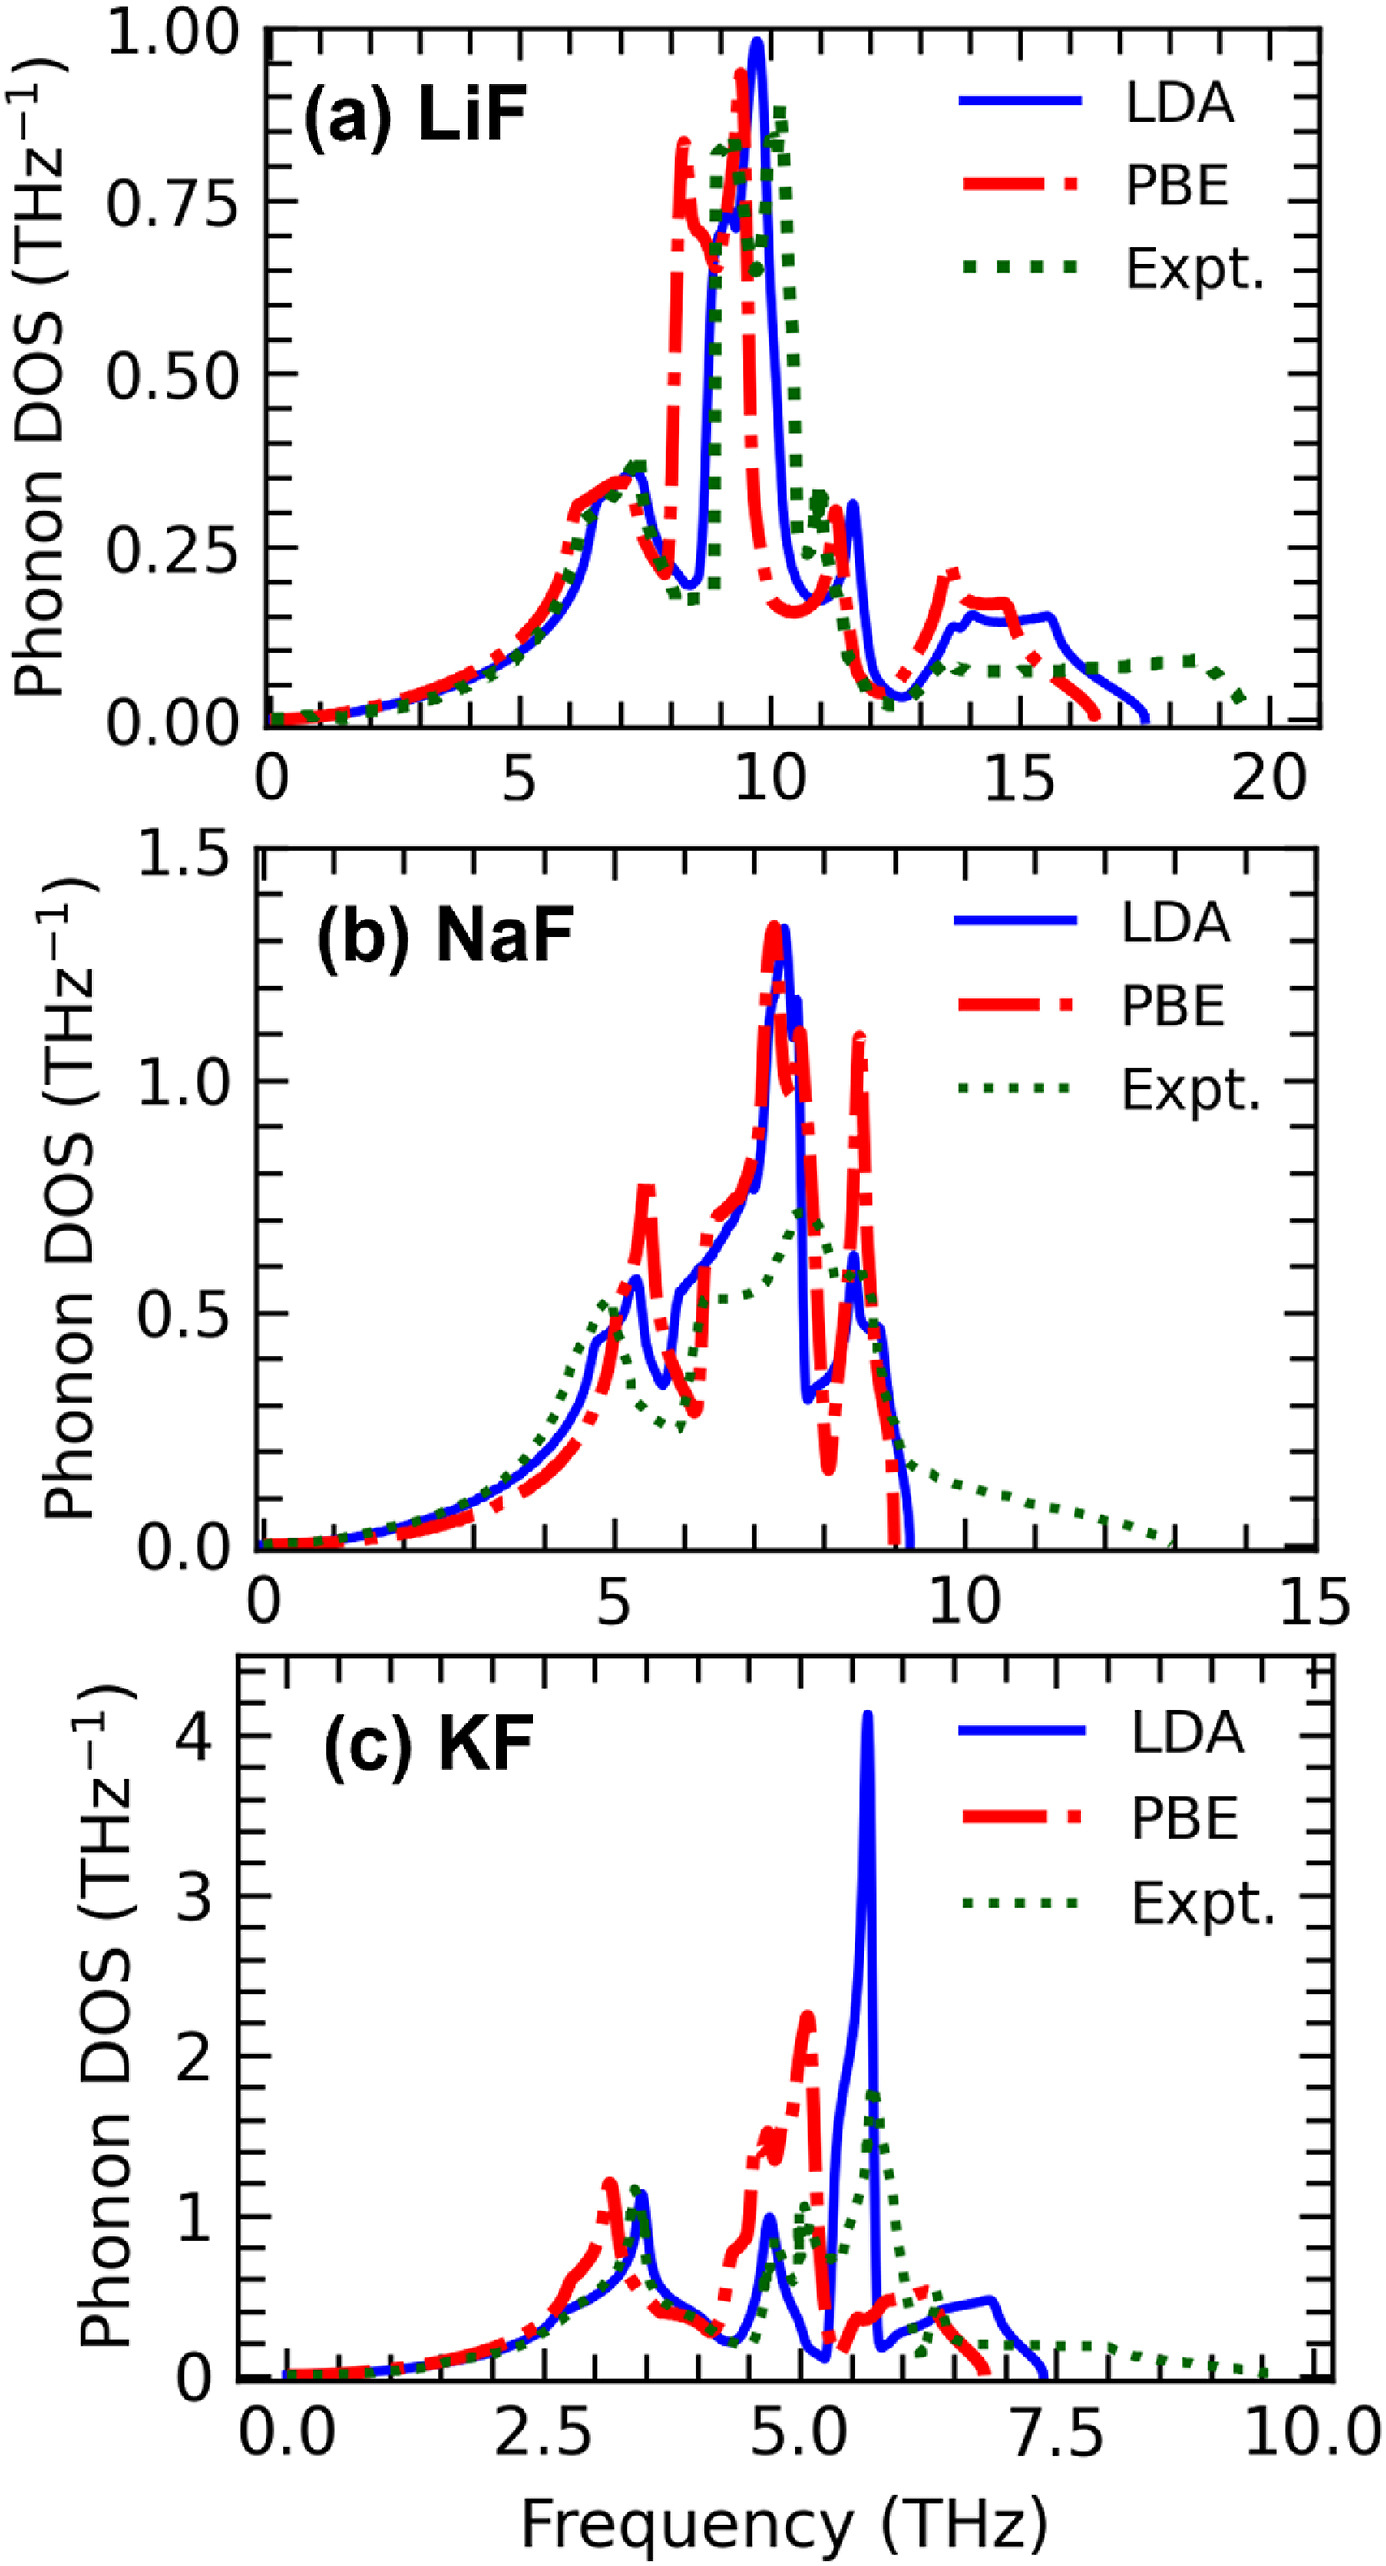
\includegraphics[width=0.45\linewidth]{moltensalts/Moltensalts-FLiNaKCr-PhononDOS.jpg}
    \caption{Predicted phonon density of states (DOS) of (a) LiF, (b) NaF, and (c) KF from DFT-based phonon calculations in comparison with phonon DOS from experiments \cite{dolling1968lattice, buhrer1970lattice, karo1969lattice}. Blue lines show results from the LDA approach, red dot-dashed lines show results from the GGA-PBE approach, and the green dotted lines are results from experiments \cite{dolling1968lattice, buhrer1970lattice, karo1969lattice}. }
    \label{ms:fig:FLiNaKCrphonon}
\end{figure}

Figure \ref{ms:fig:FLiNaKCr-Benchmark} illustrates a comparison of the predicted heat capacity (C$_p$), entropy (S), and enthalpy (H$-$H$_{300}$) of LiF, NaF, and KF in terms of the phonon-based QHA, where the DFT calculations were conducted using both the LDA and GGA, and the predicted results are compared to the data from the SSUB database \cite{sgteurl}. In general, thermodynamic properties predicted by LDA align well with the results from SSUB. The most substantial difference between LDA and SSUB is the C$_p$ values of KF, where a 6\% disparity is noted. Furthermore, these comparisons reveal that the LDA results exhibit a better agreement with SSUB than the GGA results, particularly for LiF. For example, at 1100 K, the C$_p$ values predicted by LDA demonstrate only a 2\% difference compared to those from the SSUB \cite{sgteurl}, whereas an 18\% difference is observed when using GGA. Figure \ref{ms:fig:FLiNaKCr-Benchmark} indicates that the QHA in terms of LDA yields more reliable predictions of thermodynamic properties in LiF-NaF-KF-based system, agreeing with the observations in phonon DOS in Figure \ref{ms:fig:FLiNaKCrphonon}. Subsequent DFT calculations were hence performed using the LDA approach. 

\begin{figure}[ht]
    \centering
    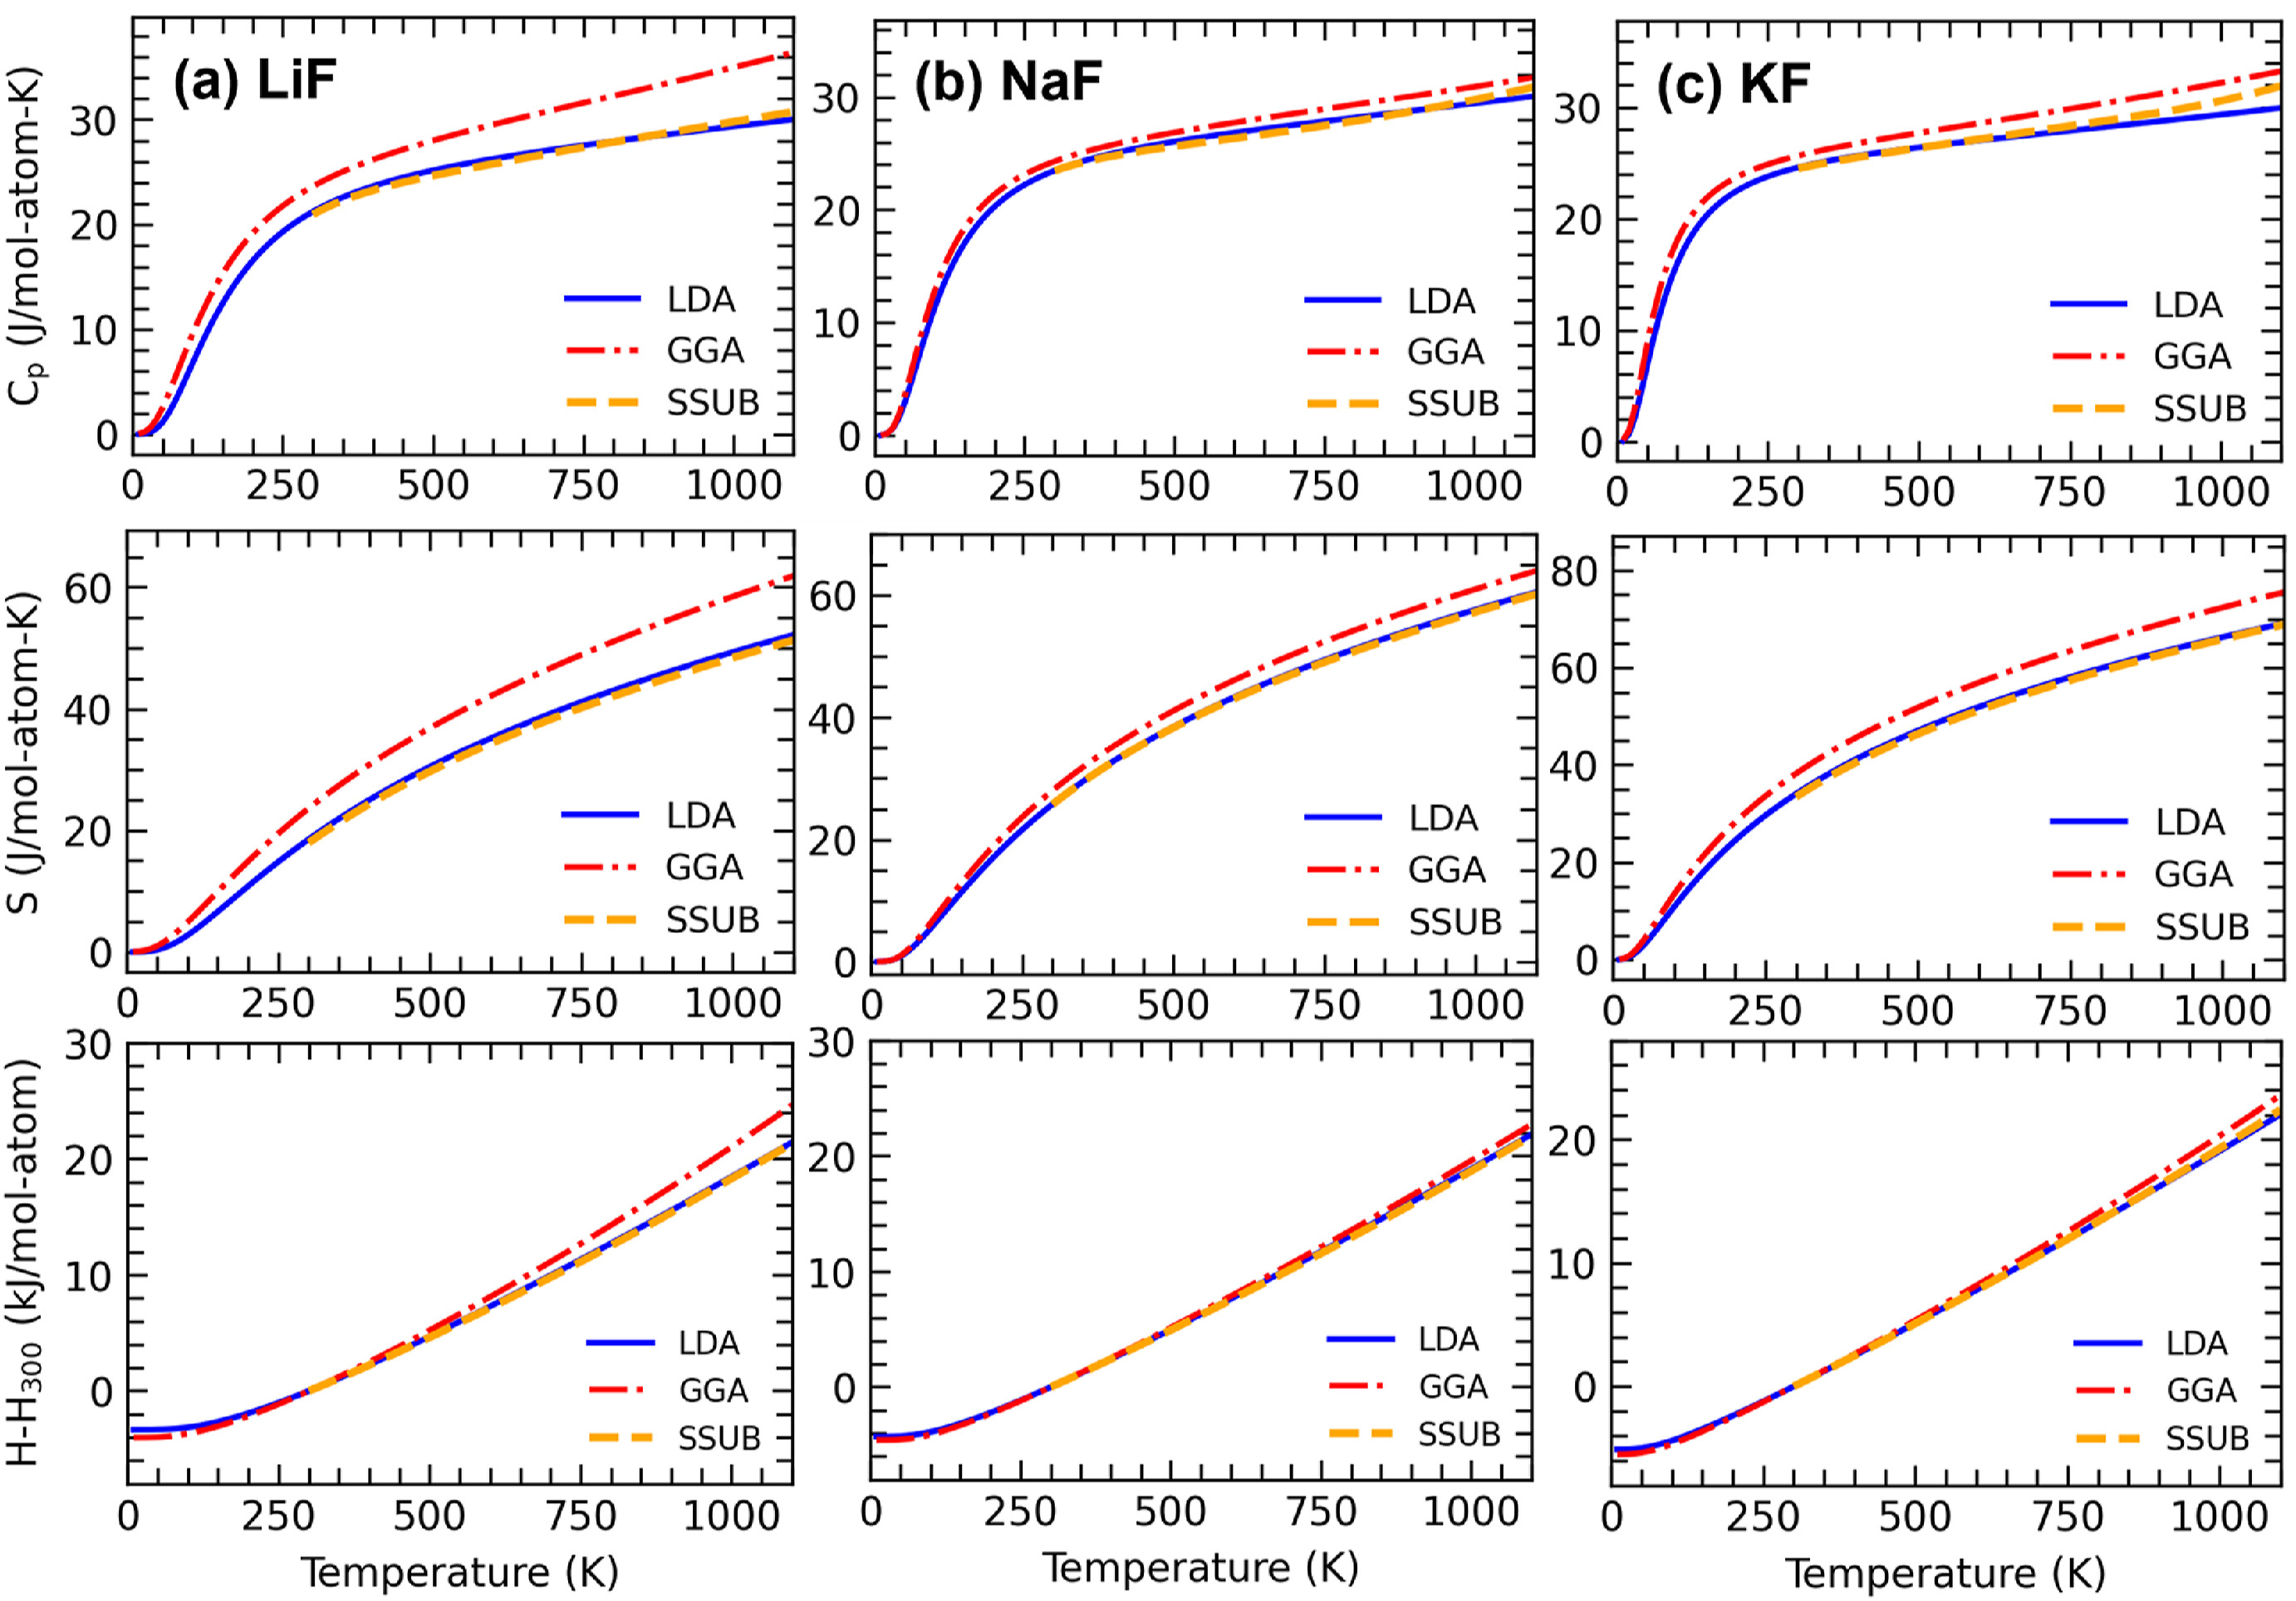
\includegraphics[width=1\linewidth]{moltensalts/Moltensalts-FLiNaKCr-Benchmark.jpg}
    \caption{Predicted heat capacity C$_p$, entropy S, and enthalpy with reference at 300 K (H$-$H$_{300}$) of (a) LiF, (b) NaF, and (c) KF by DFT-based QHA via phonon calculations. Results by LDA is marked as solid blue lines, calculations by PBE are marked as dashed dot red lines, and the SSUB results \cite{sgteurl} are in dashed yellow lines. The SSUB results are implemented in the present modeling work.}
    \label{ms:fig:FLiNaKCr-Benchmark}
\end{figure}

Figure \ref{ms:fig:FLiNaKCr-Benchmark-Cr} shows the present DFT predictions and the values in SSUB \cite{sgteurl} regarding C$_p$, S, and H$-$H$_{300}$ for CrF$_3$ and CrF$_2$. In general, the present predictions tend to be lower than those obtained from SSUB \cite{sgteurl}. For CrF$_3$, the DFT predicted C$_p$ = 19.77 J/mol-atom-K closely aligns with the SSUB value of 19.73 J/mol-atom-K at 300 K. As the temperature increases to 1300 K, the difference increases to 9\%. Similarly, for CrF$_2$, the C$_p$ = 21.22 J/mol-atom-K at 300 K by DFT is in good agreement with the value of 21.66 from SSUB. At a higher temperature of 1140 K, the difference expands to 12\%. Regarding entropy, DFT predicts lower S values for both CrF$_3$ and CrF$_2$ than those in SSUB across the temperature range shown in Figure \ref{ms:fig:FLiNaKCr-Benchmark-Cr}. At high temperatures (e.g., 1600 K for CrF$_3$ and 1140 K for CrF$_2$), it shows a 10\% difference in CrF$_3$ and 14\% in CrF$_2$. It is found that a good agreement is observed regarding H$-$H$_{300}$ values of CrF$_3$ and CrF$_2$ between the DFT calculations and the SSUB at lower temperatures (< 1000 K for CrF$_3$ and < 600 K for CrF$_2$). H$-$H$_{300}$ from DFT becomes slightly lower than that in SSUB \cite{sgteurl} with increasing temperature, with the differences, for example, around 5\% in CrF$_3$ at 1650 K and 9\% in CrF$_2$ at 1140 K.

\begin{figure}[ht]
    \centering
    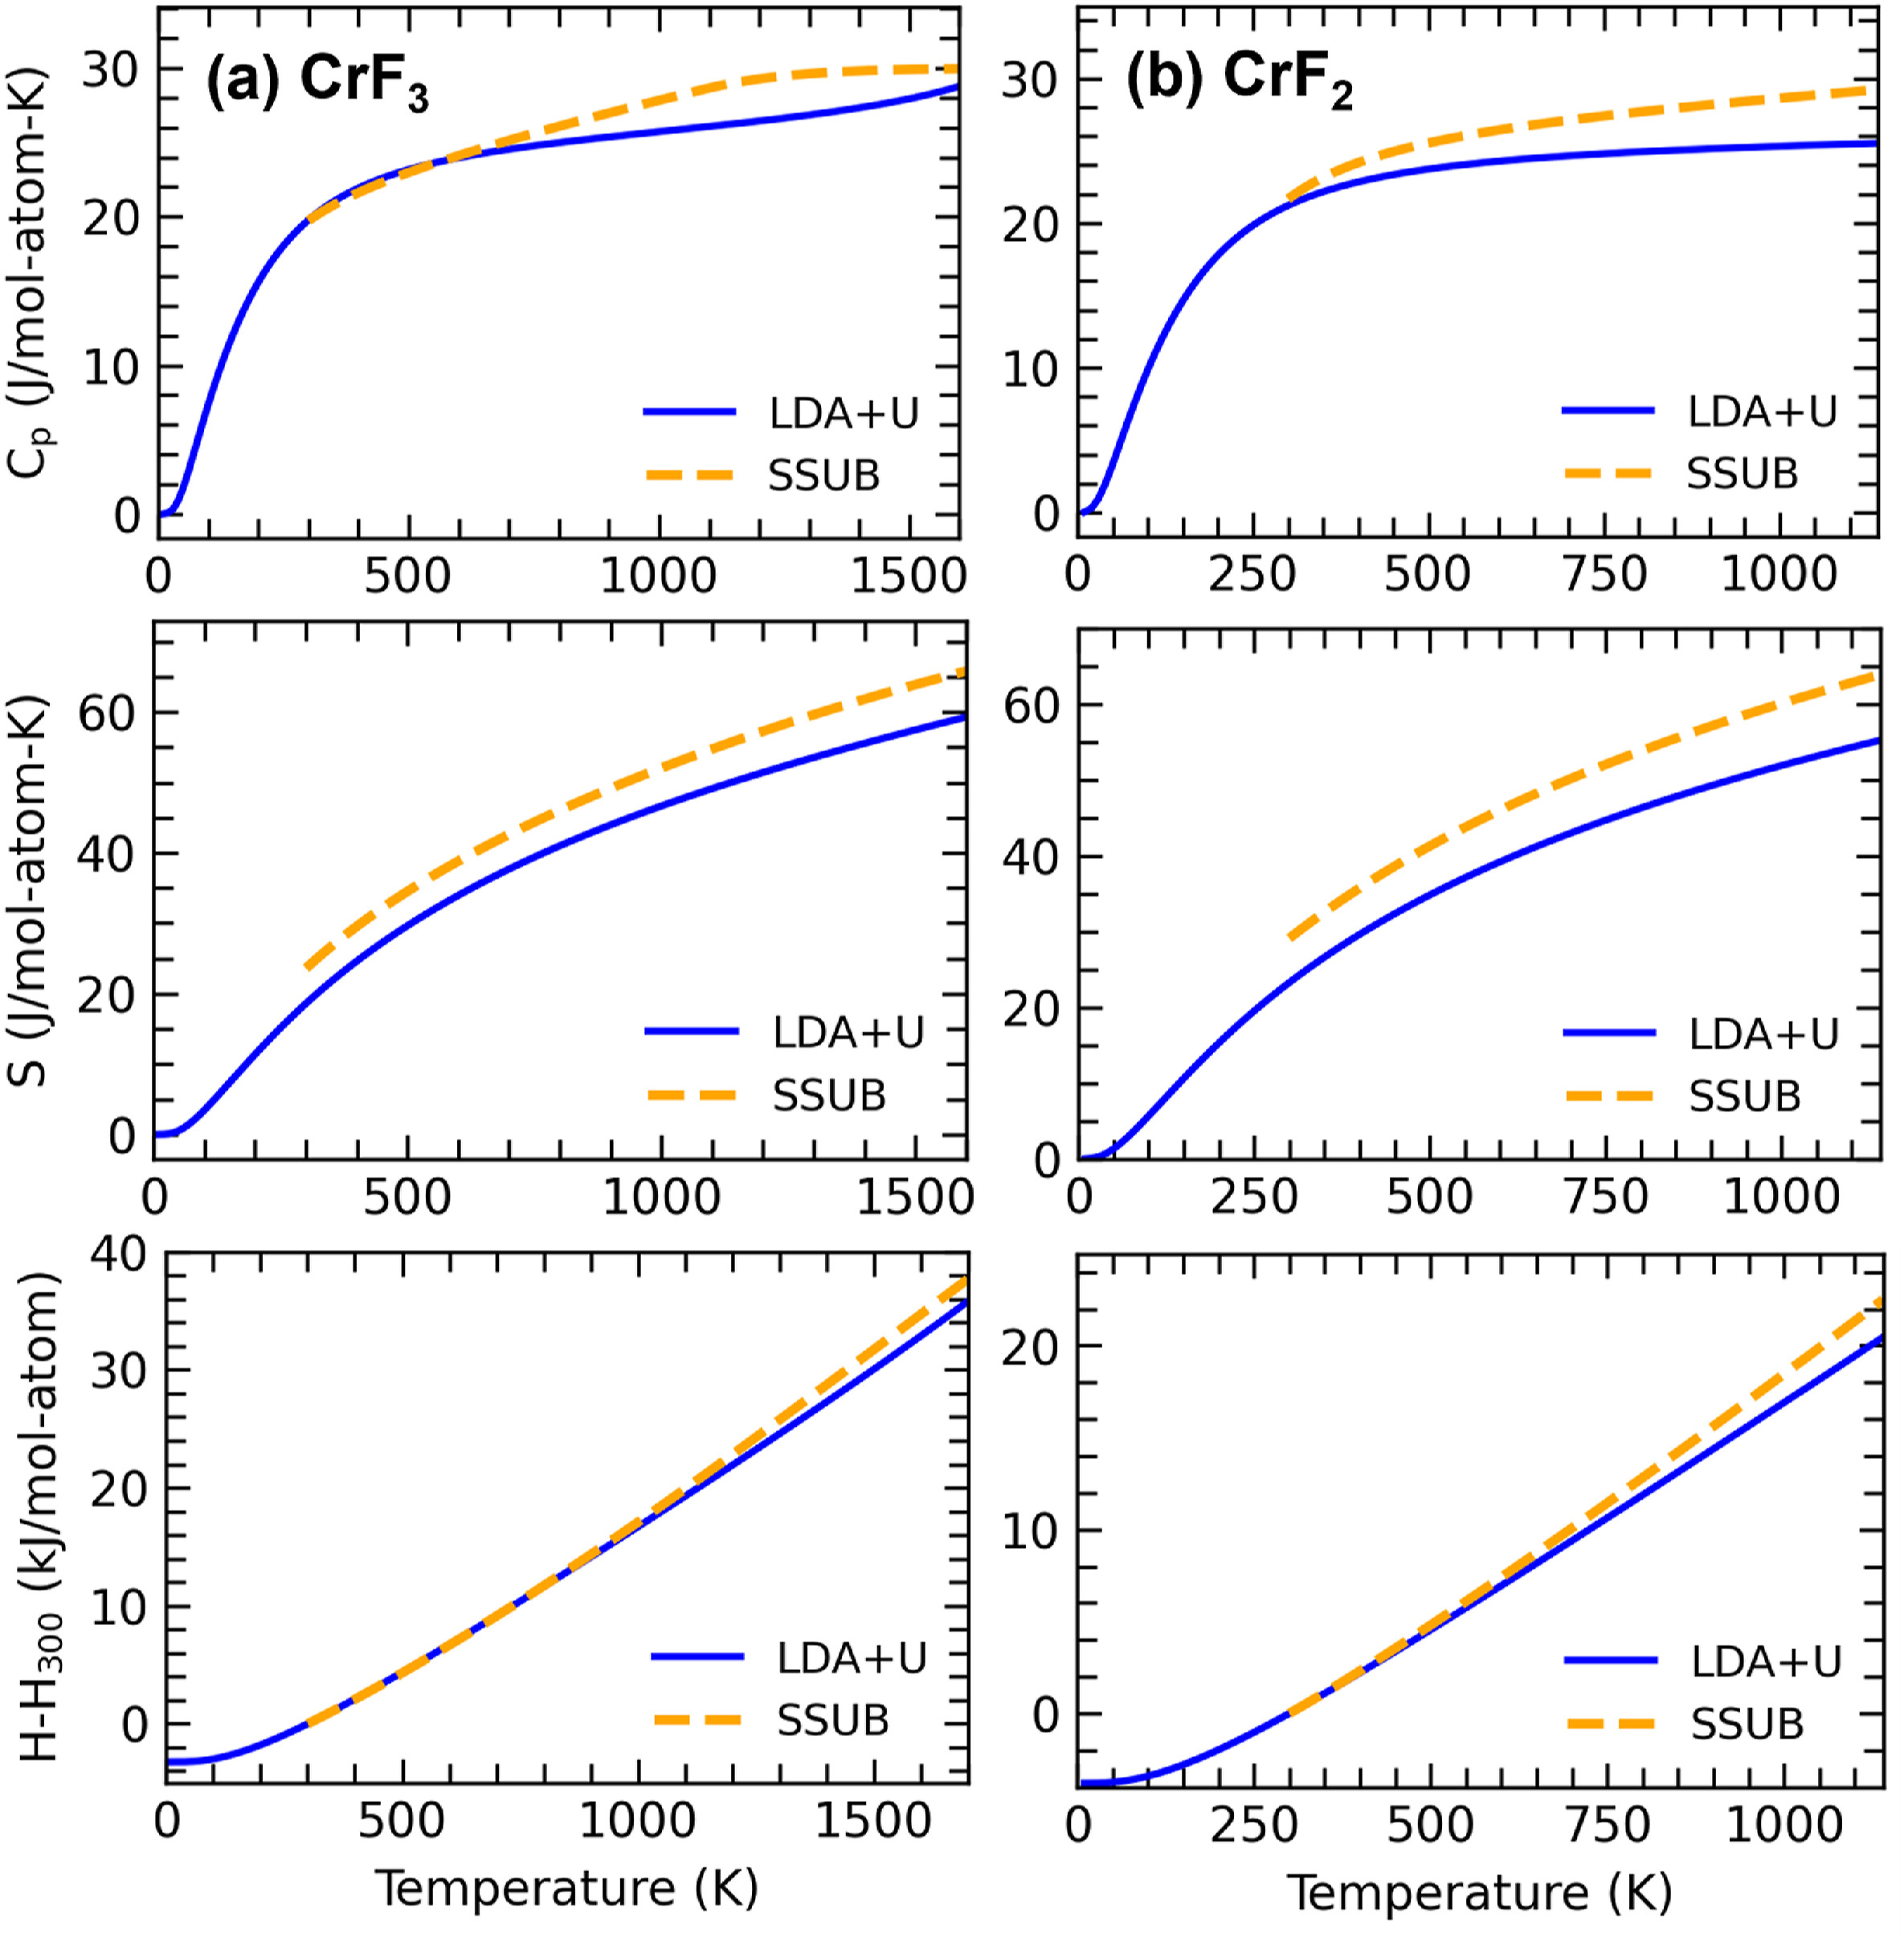
\includegraphics[width=0.75\linewidth]{moltensalts/Moltensalts-FLiNaKCr-Benchmark-Cr.jpg}
    \caption{Predicted heat capacity C$_p$, entropy S, and enthalpy with reference at 300 K (H$-$H$_{300}$) of (a) CrF$_3$ and (b) CrF$_2$ by DFT-based QHA via phonon calculations marked in solid lines in comparison with SSUB \cite{sgteurl} in dashed lines.}
    \label{ms:fig:FLiNaKCr-Benchmark-Cr}
\end{figure}

Table \ref{ms:tab:FLiNaK-Cr-Hf} shows the present DFT values of formation enthalpy ($\Delta_fH_m$) of these ternary compounds using the LDA+U approach, together with the reactions to form these compounds. Table \ref{ms:tab:FLiNaK-Cr-Hf} shows that the $\Delta_fH_m$ values are negative for all ternary compounds with reference to their corresponding binary compounds. Yin et al. \cite{yin2018thermodynamic, yin2014thermodynamic} conducted DFT calculations for Li$_3$CrF$_6$ and Na$_3$CrF$_6$. Predicted $\Delta_fH_m$ values from the Materials Project \cite{jain2013commentary} and the Open Quantum Materials Database (OQMD) \cite{kirklin2015open} are also listed in Table \ref{ms:tab:FLiNaK-Cr-Hf} and displayed in Figure \ref{ms:fig:FLiNaKCr-Hf}. The present DFT calculations by LDA+U predict higher $\Delta_fH_m$ values of Li$_3$CrF$_6$ and Na$_3$CrF$_6$ than those by Yin et al. \cite{yin2018thermodynamic, yin2014thermodynamic} using GGA. The present DFT calculations align better with results from the Materials Project \cite{jain2013commentary} and OQMD \cite{kirklin2015open} than calculations from Yin et al. \cite{yin2018thermodynamic, yin2014thermodynamic}. Figure \ref{ms:fig:FLiNaKCr-Hf} displays the convex hulls for the LiF-CrF$_3$, NaF-CrF$_3$, and KF-CrF$_3$ systems based on the $\Delta_fH_m$ values listed in Table \ref{ms:tab:FLiNaK-Cr-Hf}. These convex hulls serve as indicators regarding the stability of ternary compounds in these systems. Li$_3$CrF$_6$ is on the convex hull, suggesting that it is stable in the LiF-CrF$_3$ system. In the NaF-CrF$_3$ system, Na$_3$CrF$_6$ is located on the hull, indicating its stability at 0 K. Na$_5$Cr$_3$F$_{14}$ shows an elevation of 1.09 kJ/mol-atom above the hull, and NaCrF$_4$ shows 0.42 kJ/mol-atom above the hull. In the KF-CrF$_3$ system, K$_2$CrF$_5$ is on the convex hull at 0 K. K$_2$Cr$_5$F$_{17}$ is the farthest away from the convex hull (1.31 kJ/mol-atom above it), while K$_3$CrF$_6$ and KCrF$_4$ are 0.62 kJ/mol-atom and 0.61 kJ/mol-atom above the hull, respectively. These calculations at 0 K suggest that Na$_5$Cr$_3$F$_{14}$, NaCrF$_4$, K$_2$Cr$_5$F$_{17}$, K$_3$CrF$_6$, and KCrF$_4$ are not stable at 0 K, while De Kozak \cite{DeKozak1969} reported the existence of the above ternary compounds at high temperature. It suggests that phonon-based QHA is necessary to investigate the thermodynamic properties of ternary compounds at high temperatures.

\begin{figure}[H]
    \centering
    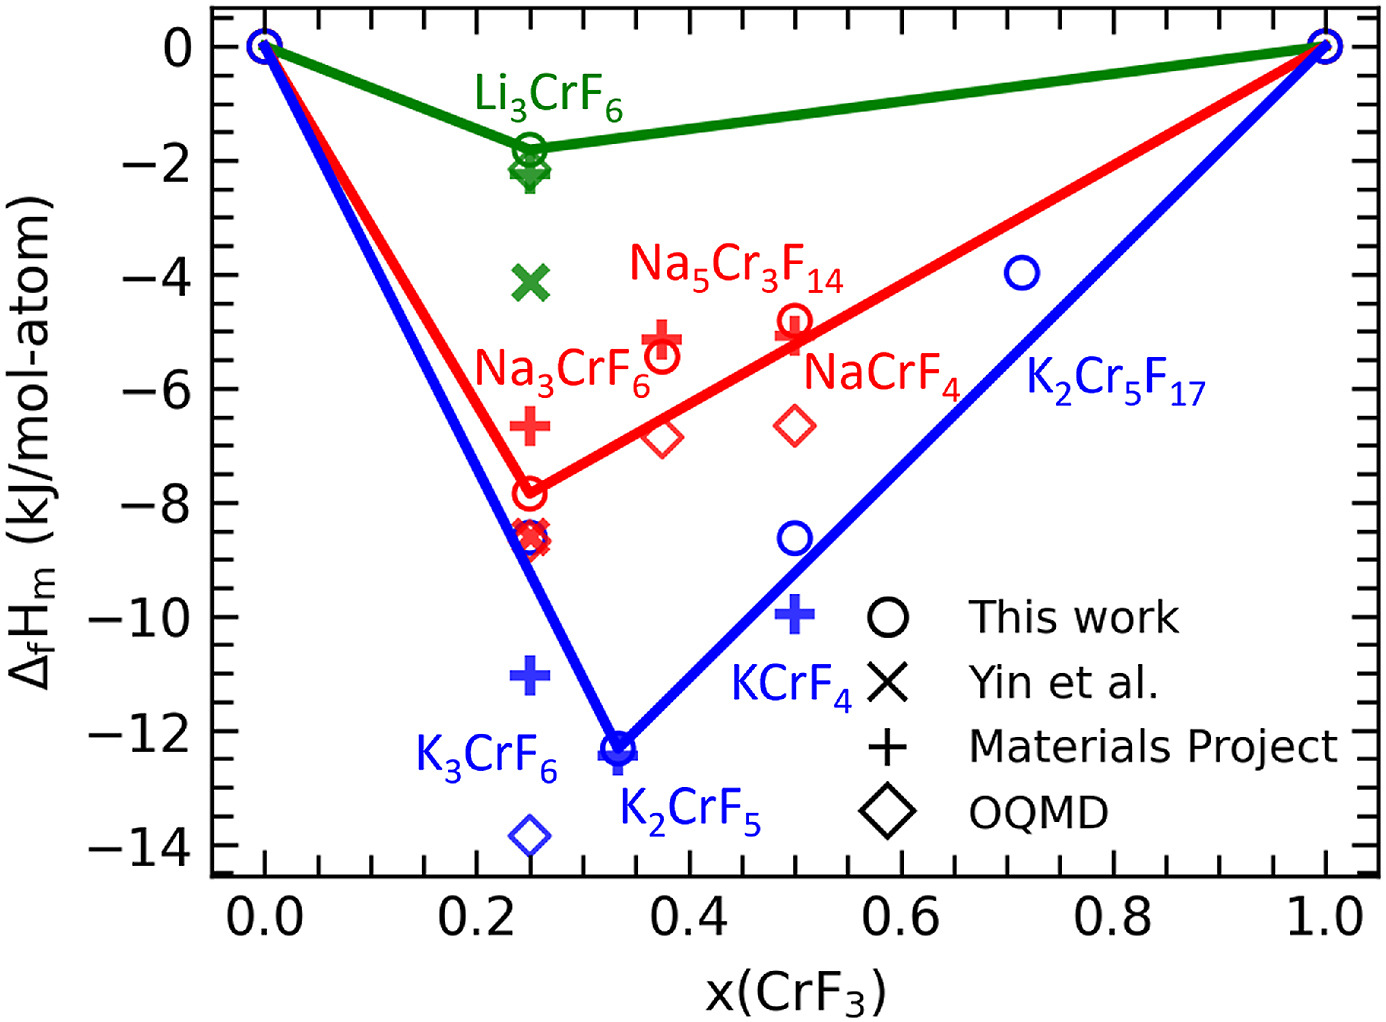
\includegraphics[width=0.5\linewidth]{moltensalts/Moltensalts-FLiNaKCr-DFTHf.jpg}
    \caption{Convex hull of ternary compounds in LiF-CrF$_3$ (green), NaF-CrF$_3$ (red), and KF-CrF$_3$ (blue) at 0 K from DFT-based calculations from the present work. Circles ($\circ$) are the formation enthalpy of compounds from the present work; cross markers ($\times$) are the formation enthalpy of compounds from Yin et al. \cite{yin2018thermodynamic, yin2014thermodynamic}; plus markers ($+$) result from The Materials Project \cite{jain2013commentary}; and diamond markers ($\diamond$) results from OQMD \cite{kirklin2015open}. }
    \label{ms:fig:FLiNaKCr-Hf}
\end{figure}

\begin{table}[H]
    \centering
    \caption{DFT-based results of formation enthalpy ($\Delta_fH_m$) at 0 K of ternary compounds in the AF-CrF$_3$ (A=Li, Na, and K) systems with the reference states as shown in the reactions. DFT results from Yin et al. \cite{yin2018thermodynamic, yin2014thermodynamic}, the Materials Project \cite{jain2013commentary}, and the Open Quantum Materials Database (OQMD) \cite{kirklin2015open} are listed for comparison.}
    \begin{tabular}{>{\raggedright\arraybackslash}m{2.5cm}>{\raggedright\arraybackslash}m{5cm}>{\raggedright\arraybackslash}m{3cm}>{\raggedright\arraybackslash}m{5cm}}
    \hline
    \textbf{Compound}&\textbf{Reaction}&\textbf{$\Delta_fH_m$ (J/mol-atom)}&\textbf{Source}\\
    \hline
    Li$_3$CrF$_6$&Li$_3$CrF$_6$$=$3LiF$+$CrF$_3$&$-1815$&This work\\
    &&$-4144$&Yin et al. \cite{yin2014thermodynamic}\\
    &&$-2238$&Materials Project \cite{jain2013commentary}\\
    &&$-2161$&OQMD \cite{kirklin2015open}\\
    Na$_3$CrF$_6$&Na$_3$CrF$_6$$=$3NaF$+$CrF$_3$&$-7849$&This work\\
	&&$-8592$&Yin et al. \cite{yin2018thermodynamic}\\
    &&$-6657$&Materials Project \cite{jain2013commentary}\\
    &&$-8683$&OQMD \cite{kirklin2015open}\\
    Na$_3$CrF$_6$&Na$_3$CrF$_6$$=$3NaF$+$CrF$_3$&$-7849$&This work\\
	&&$-8592$&Yin et al. \cite{yin2018thermodynamic}\\
    &&$-6657$&Materials Project  \cite{jain2013commentary}\\
    &&$-8683$&OQMD \cite{kirklin2015open}\\
    Na$_5$Cr$_3$F$_{14}$&Na$_5$Cr$_3$F$_{14}$$=$5NaF$+$3CrF$_3$&$-5447$&This work\\
	&&$-5148$&Materials Project \cite{jain2013commentary}\\
	&&$-6859$&OQMD \cite{kirklin2015open}\\
    NaCrF$_4$&NaCrF$_4$$=$NaF$+$CrF$_3$&$-4816$&This work\\
    &&$-5071$&Materials Project \cite{jain2013commentary}\\
	&&$-6657$&OQMD \cite{kirklin2015open}\\
    K$_3$CrF$_6$&K$_3$CrF$_6$$=$3KF$+$CrF$_3$&$-8621$&This work\\
    &&$-11038$&Materials Project \cite{jain2013commentary}\\
	&&$-13855$&OQMD \cite{kirklin2015open}\\
    K$_2$CrF$_5$&K$_2$CrF$_5$$=$2KF$+$CrF$_3$&$-12322$&This work\\
	&&$-12446$&Materials Project \cite{jain2013commentary}\\
    KCrF$_4$&KCrF$_4$$=$KF$+$CrF$_3$&$-8631$&This work\\
    &&$-9970$&Materials Project \cite{jain2013commentary}\\
    K$_2$Cr$_5$F$_{17}$&K$_2$Cr$_5$F$_{17}$$=$2KF$+$5CrF$_3$&$-3974$&This work\\
    \hline
    \end{tabular}
    \label{ms:tab:FLiNaK-Cr-Hf}
\end{table}

\begin{figure}[H]
    \centering
    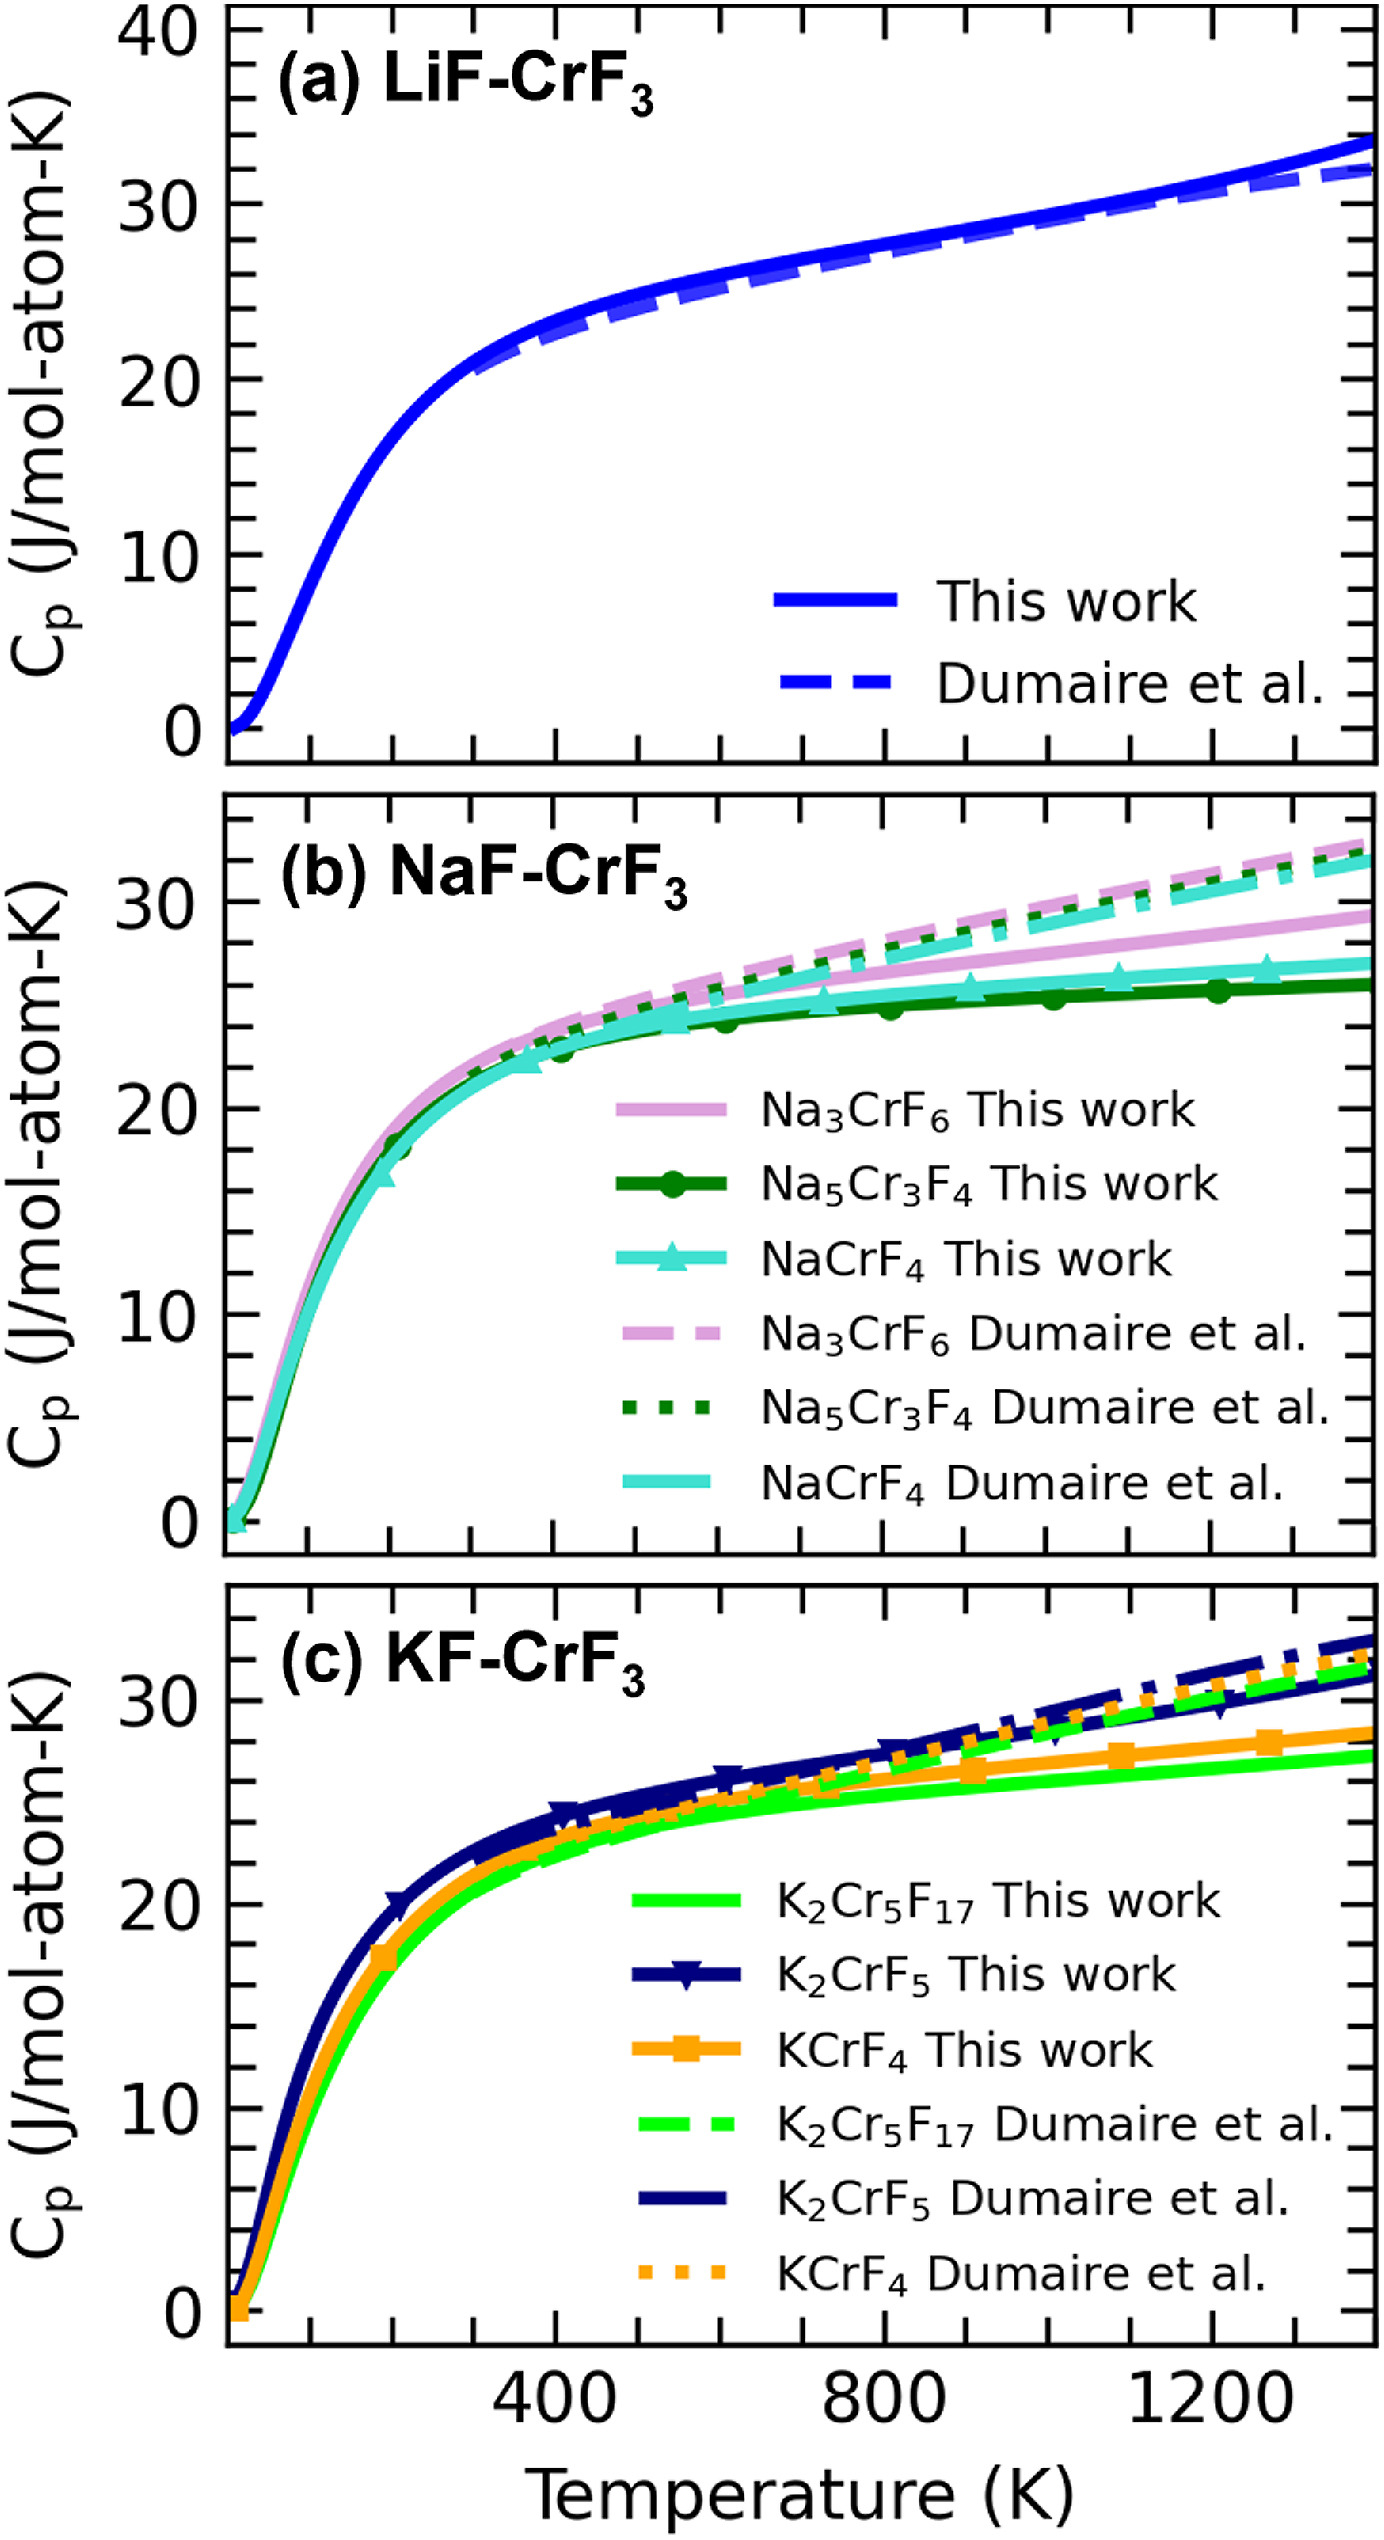
\includegraphics[width=0.45\linewidth]{moltensalts/Moltensalts-FLiNaKCr-DFTcompounds.jpg}
    \caption{Predicted heat capacities of ternary compounds in the (a) LiF–CrF$_3$, (b) NaF–CrF$_3$, and (c) KF-CrF$_3$ systems by DFT-based QHA via phonon calculations (solid lines) compared with the Dumaire et al. \cite{dumaire2021thermodynamic}'s work (dashed lines). The QHA results are implemented in the present modeling work for ternary compounds.}
    \label{ms:fig:FLiNaKCr-DFTcompounds}
\end{figure}

Figure \ref{ms:fig:FLiNaKCr-DFTcompounds} shows the predicted heat capacities C$_p$ of ternary compounds in the AF-CrF$_3$ (A= Li, Na, and K) systems from the phonon-based QHA, in comparison with the results estimated by the Neumann-Kopp rule \cite{leitner2010application}, which were used in CALPHAD modeling by Dumaire et al. \cite{dumaire2021thermodynamic}. It shows that the Neumann-Kopp rule matches the results of phonon-based QHA in the LiF-CrF$_3$ system. However, in the NaF-CrF$_3$ and KF-CrF$_3$ systems, the Neumann-Kopp rule estimates higher values of C$_p$ with respect to the values predicted by phonon-based QHA. The differences between the LiF-CrF$_3$ system and the NaF/KF-CrF$_3$ may be attributed to variations in melting temperatures between ternary and corresponding binary compounds. For example, in the LiF-CrF$_3$ system, the melting temperature of Li$_3$CrF$_6$ is reported at 1129 K \cite{DeKozak1969}, which is close to that of LiF at 1121 K and below that of CrF$_3$ at 1698 K \cite{sgteurl}. Considering the temperature below the melting point of Li$_3$CrF$_6$ (T < 1129 K), there are reliable resources of C$_p$ data from two endmembers LiF and CrF$_3$, thus the Neumann-Kopp rule C$_p$ estimation of Li$_3$CrF$_6$ is acceptable. However, in the NaF-CrF$_3$ system, Na$_3$CrF$_6$ melts at 1413 K \cite{DeKozak1969}, while NaF melts at 1269 K \cite{sgteurl}, indicating that there is an approximately 150 K temperature range without reliable C$_p$ data for NaF. In contrast, the phonon-based calculations are direct predictions of ternary compounds and they provide more accurate descriptions of thermodynamic properties for compounds than those by the Neumann-Kopp rule used by Dumaire et al. \cite{dumaire2021thermodynamic}, especially at high temperatures. Therefore, the phonon-based QHA results were used in the present CALPHAD modeling to improve the accuracy in describing ternary compounds. Note that the C$_p$ values for compounds in the (LiF, NaF, KF, and CrF$_2$)-CrF$_3$ systems can be predicted using the Supplementary XML file \cite{gong2024revisiting}.

\subsection{Thermodynamic modeling of the (LiF, NaF, KF, CrF$_2$)-CrF$_3$ system} \label{moltensalts:ssec:FLiNaKCrmodeling}

Figure \ref{ms:fig:FLiNaKCr-Phasediagram} shows the phase diagrams of the (LiF, NaF, KF, and CrF$_2$)-CrF$_3$ systems calculated from present models and compared with experimental data by De Kozak \cite{de1975systeme, DeKozak1969} and Sturm \cite{sturm1962phase}. The present CALPHAD modeling shows a good agreement regarding phase boundaries with experimental data. The presently modeled parameters for liquid and the complete thermodynamic database can be found in the Supplementary XML file \cite{gong2024revisiting}. Details of the invariant reactions and the congruent melting temperature calculated from the present modeling work compared to experiments \cite{de1975systeme, DeKozak1969, sturm1962phase} and ML predictions using Hong et al.’s model \cite{hong2022melting} are listed in Table \ref{ms:tab:FLiNaK-Cr-inv} with discussion below. 

In the LiF-CrF$_3$ system, the present prediction of the eutectic reaction Liquid $\leftrightarrow$ CrF$_3$ + Li$_3$CrF$_6$ at T = 1056 K matches closely with experimental values of T = 1059 K \cite{DeKozak1969}. There is a minor difference of 1 K observed for Liquid $\leftrightarrow$ LiF + Li$_3$CrF$_6$, with the present modeling predicts an eutectic temperature of 1002 K compared to 1003 K reported by De Kozak \cite{DeKozak1969}. This presents an improvement over the 1008 K predicted by Dumaire et al. \cite{dumaire2021thermodynamic}’s modeling. The present prediction of the congruent melting temperature of 1131 K is 2 K higher than the experimental value of 1129 K reported by De Kozak \cite{DeKozak1969}, significantly improved from the prediction of 1111 K by Dumaire et al. \cite{dumaire2021thermodynamic}. 

\begin{figure}[H]
    \centering
    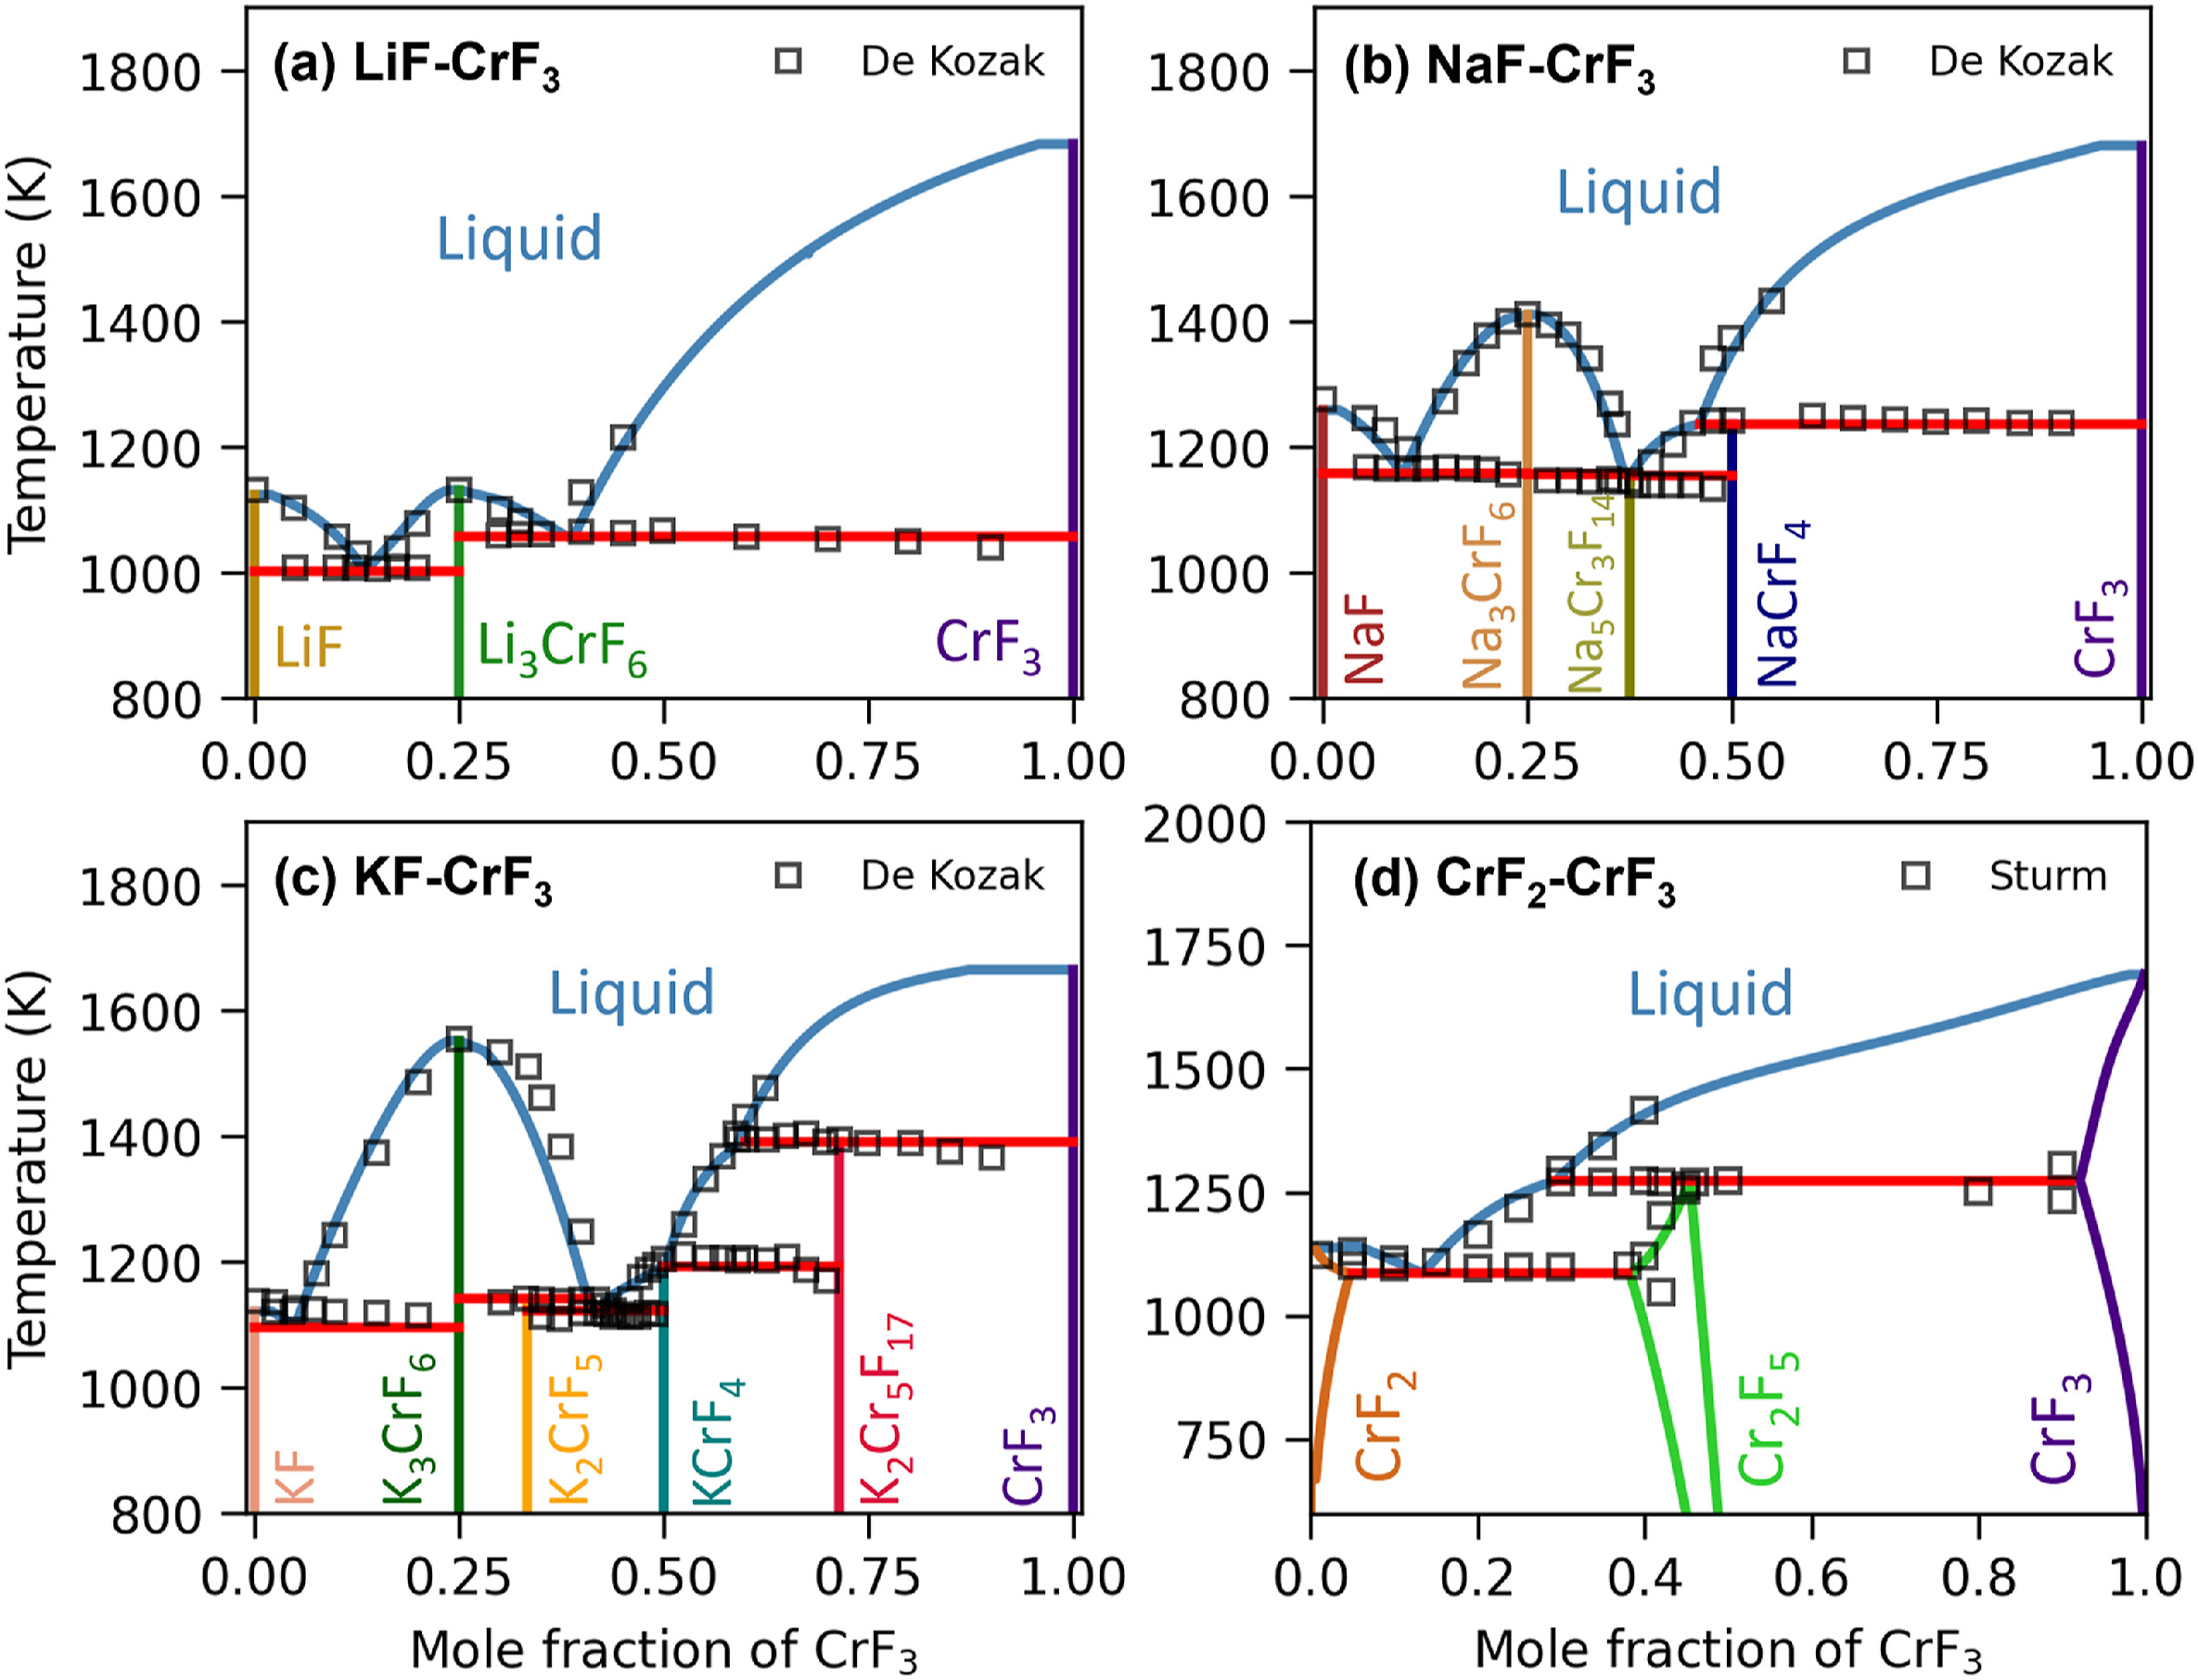
\includegraphics[width=0.9\linewidth]{moltensalts/Moltensalts-FLiNaKCr-Phasediagram.jpg}
    \caption{Predicted phase diagrams of the (a) LiF–CrF$_3$, (b) NaF–CrF$_3$, (c) KF-CrF$_3$, and (d) CrF$_2$–CrF$_3$ systems by the present CALPHAD modeling in comparison with experimental data \cite{de1975systeme, DeKozak1969, sturm1962phase}.}
    \label{ms:fig:FLiNaKCr-Phasediagram}
\end{figure}

\begingroup
\renewcommand\arraystretch{0.8}
\begin{longtable}[H]{>{\raggedright\arraybackslash}m{2cm}>{\raggedright\arraybackslash}m{6cm}>{\raggedright\arraybackslash}m{1.5cm}>{\raggedright\arraybackslash}m{3cm}>{\raggedright\arraybackslash}m{3.5cm}}
    \caption{Predicted invariant equilibria in the AF-CrF$_3$ (A=Li, Na, K) systems by the present CALPHAD modeling, compared with experimental data from De Kozak \cite{DeKozak1969} and Sturm \cite{sturm1962phase} (marked with *), and other modeling works \cite{yin2014thermodynamic, yin2015thermodynamic, yin2018thermodynamic, dumaire2021thermodynamic}.}\\
    \hline
    \textbf{Reaction}&&\textbf{$x$(CrF$_3$)}&\textbf{Temperature (K)}&\textbf{Source}\\
    \hline
    Eutectic&Liquid$\leftrightarrow$LiF+Li$_3$CrF$_6$&0.135&1002&This work\\
    &&0.150&1003&De Kozak \cite{DeKozak1969}$^*$\\
    &&0.136&1008&Dumaire et al. \cite{dumaire2021thermodynamic}\\
    &&0.148&1003&Yin et al. \cite{yin2014thermodynamic}\\
    Melting&Liquid$\leftrightarrow$Li$_3$CrF$_6$&0.25&1131&This work\\
    &&0.25&1129&De Kozak \cite{DeKozak1969}$^*$\\
    &&0.25&1114&Hong et al. \cite{hong2022melting}\\
    &&0.25&1111&Dumaire et al. \cite{dumaire2021thermodynamic}\\
    &&0.25&1125&Yin et al. \cite{yin2014thermodynamic}\\
    Eutectic&Liquid$\leftrightarrow$CrF$_3$+Li$_3$CrF$_6$&0.382&1056&This work\\
    &&0.350&1059&De Kozak \cite{DeKozak1969}$^*$\\
    &&0.363&1062&Dumaire et al. \cite{dumaire2021thermodynamic}\\
    &&0.354&1058&Yin et al. \cite{yin2014thermodynamic}\\
    Eutectic&Liquid$\leftrightarrow$NaF+Na$_3$CrF$_6$&0.098&1155&This work\\
    &&0.123&1166&De Kozak \cite{DeKozak1969}$^*$\\
    &&0.106&1175&Dumaire et al. \cite{dumaire2021thermodynamic}\\
    &&0.114&1162&Yin et al. \cite{yin2018thermodynamic}\\
    Melting&Liquid$\leftrightarrow$Na$_3$CrF$_6$&0.25&1410&This work\\
    &&0.25&1413&De Kozak \cite{DeKozak1969}$^*$\\
    &&0.25&1404&Hong et al. \cite{hong2022melting}\\
    &&0.25&1385&Dumaire et al. \cite{dumaire2021thermodynamic}\\
    &&0.25&1416&Yin et al. \cite{yin2018thermodynamic}\\
    Eutectic&Liquid$\leftrightarrow$Na$_5$Cr$_3$F$_{14}$+Na$_3$CrF$_6$&0.368&1155&This work\\
    &&0.371&1145&Dumaire et al. \cite{dumaire2021thermodynamic}\\
    &&0.367&1142&Yin et al. \cite{yin2018thermodynamic}\\
    Eutectic&Liquid$\leftrightarrow$Na$_5$Cr$_3$F$_{14}$+NaCrF$_4$&0.377&1154&This work\\
    &&0.381&1144&Dumaire et al. \cite{dumaire2021thermodynamic}\\
    &&0.383&1141&Yin et al. \cite{yin2018thermodynamic}\\
    Peritectic&Liquid+CrF$_3$$\leftrightarrow$NaCrF$_4$&0.5&1235&This work\\
    &&0.5&1234&De Kozak \cite{DeKozak1969}$^*$\\
    &&0.5&1232&Dumaire et al. \cite{dumaire2021thermodynamic}\\
    &&0.5&1239&Yin et al. \cite{yin2018thermodynamic}\\
    Eutectic&Liquid$\leftrightarrow$KF+K$_3$CrF$_6$&0.050&1096&This work\\
    &&0.048&1115&De Kozak \cite{DeKozak1969}$^*$\\
    &&0.041&1108&Dumaire et al. \cite{dumaire2021thermodynamic}\\
    &&0.045&1113&Yin et al. \cite{yin2018thermodynamic}\\ 
    Melting&Liquid$\leftrightarrow$K$_3$CrF$_6$&0.25&1551&This work\\
    &&0.25&1553&De Kozak \cite{DeKozak1969}$^*$\\
    &&0.25&1520&Hong et al. \cite{hong2022melting}\\
    &&0.25&1553&Dumaire et al. \cite{dumaire2021thermodynamic}\\
    &&0.25&1548&Yin et al. \cite{yin2015thermodynamic}\\ 
    Peritectic&Liquid+K$_3$CrF$_6$$\leftrightarrow$K$_2$CrF$_5$&0.333&1141&This work\\
    &&0.333&1133&De Kozak \cite{DeKozak1969}$^*$\\
    &&0.333&1130&Dumaire et al. \cite{dumaire2021thermodynamic}\\
    &&0.333&1135&Yin et al. \cite{yin2015thermodynamic}\\  
    Eutectic&Liquid$\leftrightarrow$KCrF$_4$+K$_2$CrF$_5$&0.420&1120&This work\\
    &&0.45&1112&De Kozak \cite{DeKozak1969}$^*$\\
    &&0.432&1112&Dumaire et al. \cite{dumaire2021thermodynamic}\\
    &&0.426&1107&Yin et al. \cite{yin2015thermodynamic}\\  
    Peritectic&Liquid+K$_2$Cr$_5$F$_{17}$$\leftrightarrow$KCrF$_4$&0.5&1192&This work\\
    &&0.5&1200&De Kozak \cite{DeKozak1969}$^*$\\
    &&0.5&1191&Dumaire et al.  \cite{dumaire2021thermodynamic}\\
    &&0.5&1195&Yin et al. \cite{yin2015thermodynamic}\\ 
    Peritectic&Liquid+CrF$_3$$\leftrightarrow$K$_2$Cr$_5$F$_{17}$&0.714&1390&This work\\
    &&0.714&1390&De Kozak \cite{DeKozak1969}$^*$\\
    &&0.714&1390&Dumaire et al. \cite{dumaire2021thermodynamic}\\
    &&0.714&1388&Yin et al. \cite{yin2015thermodynamic}\\ 
    Eutectic&Liquid$\leftrightarrow$CrF$_2$+Cr$_2$F$_5$&0.134&1086&This work\\
    &&0.14&1103&Sturm \cite{sturm1962phase}$^*$\\
    &&0.115&1104&Dumaire et al. \cite{dumaire2021thermodynamic}\\
    Peritectic&Liquid+CrF$_3$$\leftrightarrow$Cr$_2$F$_5$&0.293&1273&This work\\
    &&0.29&1272&Sturm \cite{sturm1962phase}$^*$\\
    &&0.28&1271&Dumaire et al. \cite{dumaire2021thermodynamic}\\
    \hline
    \label{ms:tab:FLiNaK-Cr-inv}
\end{longtable}
\endgroup

In the NaF-CrF$_3$ system, the present modeling gives good predictions of eutectic and peritectic temperatures compared with experiments \cite{DeKozak1969}. The difference of 1 K is observed for Liquid + CrF$_3$ $\leftrightarrow$ NaCrF$_4$ (1235 K from the present work and 1234 K by De Kozak \cite{DeKozak1969}). The eutectic composition for the reaction Liquid $\leftrightarrow$ NaF + Na$_3$CrF$_6$ is $x$(CrF$_3$) = 0.098, which is around 0.025 away from the experimental value $x$(CrF$_3$) = 0.123 \cite{DeKozak1969}. The eutectic temperature for this reaction by the present modeling is 1155 K, in comparison to the experimental value of 1166 K by De Kozak \cite{DeKozak1969}. The present congruent melting temperature of Na$_3$CrF$_6$ is predicted at 1410 K, improving from the predicted 1385 K by Dumaire et al. \cite{dumaire2021thermodynamic} but slightly lower than the experimental value of 1413 K \cite{DeKozak1969}. For the two eutectic reactions without experimental data, i.e., Liquid $\leftrightarrow$ Na$_5$Cr$_3$F$_{14}$ + Na$_3$CrF$_6$ and Liquid $\leftrightarrow$ Na$_5$Cr$_3$F$_{14}$ + NaCrF$_4$, the present modeling provides similar predictions ($x$(CrF$_3$) = 0.368, T = 1155 K; $x$(CrF$_3$) = 0.377, T = 1154 K respectively) compared to those modeled by Dumaire et al. \cite{dumaire2021thermodynamic} ($x$(CrF$_3$) = 0.371, T = 1145 K; $x$(CrF$_3$) = 0.381, T = 1144 K, respectively). 

In the KF-CrF$_3$ system, the present modeling work predicts the congruent melting of K$_3$CrF$_6$ at 1551 K, which is in good agreement with the experimental value of 1553 K \cite{DeKozak1969}. For the eutectic reaction, Liquid $\leftrightarrow$ KCrF$_4$ + K$_2$CrF$_5$, the present modeling predicts $x$(CrF$_3$) = 0.42 and T = 1120 K, whereas the values are $x$(CrF$_3$) = 0.45 and T = 1112 K modeled by De Kozak \cite{DeKozak1969}. The present modeling predicts a eutectic temperature of Liquid $\leftrightarrow$ KF + K$_3$CrF$_6$ at 1096 K, slightly lower than the experimental value of 1115 K by De Kozak \cite{DeKozak1969}. For the three peritectic reactions in the KF-CrF$_3$ system, the present modeling work predicts 1141 K for Liquid + K$_3$CrF$_6$ $\leftrightarrow$ K$_2$CrF$_5$, 1192 K for Liquid + K$_2$Cr$_5$F$_{17}$ $\leftrightarrow$ KCrF$_4$, and 1390 K for Liquid + CrF$_3$ $\leftrightarrow$ K$_2$Cr$_5$F$_{17}$. These temperatures are comparable to 1133 K, 1200 K, and 1390 K, respectively, as measured by De Kozak \cite{DeKozak1969}, showing an MAE of 5.33 K.

In the CrF$_2$-CrF$_3$ system, the present modeling work improves the predicted invariant compositions. For the eutectic reaction Liquid$\leftrightarrow$CrF$_2$+Cr$_2$F$_5$, the present work predicts the eutectic point at $x$(CrF$_3$) = 0.134. This value is higher than $x$(CrF$_3$) = 0.115 by Dumaire et al. \cite{dumaire2021thermodynamic} but aligns more closely with the experimental value $x$(CrF$_3$) = 0.14 by Sturm \cite{sturm1962phase}. The eutectic temperature for this reaction is 1086 K predicted by the present modeling, demonstrating a slightly lower value of 17 K than the measured 1103 K by Sturm \cite{sturm1962phase}. For the peritectic reaction Liquid + CrF$_3$ $\leftrightarrow$ Cr$_2$F$_5$, the present work predicts $x$(CrF$_3$) = 0.293 compared to measured $x$(CrF$_3$) = 0.29 by Sturm \cite{sturm1962phase}. The present invariant temperature is predicted at 1273 K, which remains close to the experimental 1272 K by Sturm \cite{sturm1962phase}. In the present work, the single-phase region of the Cr$_2$F$_5$ solid solution phase ranges from $x$(CrF$_3$) = 0.38 to $x$(CrF$_3$) = 0.46. This range aligns well with the suggested values of $x$(CrF$_3$) from 0.40 to 0.45 by Sturm \cite{sturm1962phase}. Overall, by incorporating thermodynamic data of compounds by the present DFT calculations, the present modeling work yields improved predictions of phase diagrams.

The present CALPHAD modeling work implements the mixing enthalpy of liquid at 1700 K, which was obtained by the present AIMD simulations as described in Section \ref{moltensalts:ssec:FLiNaKCrmodel}. Note that the mixing enthalpy values from AIMD simulations can be found in the Supplementary JSON files \cite{gong2024revisiting}. Figure \ref{ms:fig:FLiNaKCr-Hmix} shows the mixing enthalpy of liquid at 1700 K by AIMD at different compositions compared to the present modeling results and results by Dumaire et al. \cite{dumaire2021thermodynamic}. It clearly shows that the mixing enthalpy of liquid (dot-dashed lines) by Dumaire et al.’s modeling \cite{dumaire2021thermodynamic} is much less negative compared to the present AIMD calculations. For example, in the LiF-CrF$_3$ system at $x$(CrF$_3$) = 0.2, AIMD predicts the mixing enthalpy of $-20.60$ kJ/mol-atom at 1700 K, while Dumaire et al’s modeling \cite{dumaire2021thermodynamic} shows $-12.65$ kJ/mol-atom, representing a 39\% higher value. Using the present AIMD data of liquid for modeling, the present modeling work (solid lines) shows a great improvement. The present modeling work improves the prediction to $-18.99$ kJ/mol-atom at $x$(CrF$_3$) = 0.2 for the LiF-CrF$_3$ system. The differences between the AIMD results and Dumaire et al.’s work \cite{dumaire2021thermodynamic} are more pronounced in the NaF-CrF$_3$ and KF-CrF$_3$ systems. In the NaF-CrF$_3$ system, at $x$(CrF$_3$) = 0.333 (a composition region near the lowest mixing enthalpy), Dumaire et al.’s modeling \cite{dumaire2021thermodynamic} shows the mixing enthalpy of $-25.45$ kJ/mol-atom, while our modeling predicts $-49.96$ kJ/mol-atom. At the same condition, AIMD gives the mixing enthalpy of $-47.37$ kJ/mol-atom, which is about 22 kJ/mol-atom lower than Dumaire et al.’s results \cite{dumaire2021thermodynamic}. In the KF-CrF$_3$ system at $x$(CrF$_3$) = 0.333, Dumaire et al. \cite{dumaire2021thermodynamic} predicts $-30.58$ kJ/mol-atom, significantly higher than $-50.20$ kJ/mol-atom by AIMD. The present modeling predicts $-53.70$ kJ/mol-atom, reducing the difference from the above-mentioned 39\% to the present 7\%. It highlights that the present AIMD simulations enhance the reliability of the present modeling in describing liquid compared to the previous work \cite{dumaire2021thermodynamic}. The mixing enthalpy (dotted lines) modeling by Yin et al. \cite{yin2018thermodynamic} in the NaF-CrF$_3$ and KF-CrF$_3$ systems agree well with the results of the present modeling. Near the low mixing enthalpy region $x$(CrF$_3$) = 0.333 in the NaF-CrF$_3$ system, Yin et al. \cite{yin2018thermodynamic} suggest the mixing enthalpy of $-40.54$ kJ/atom, which is 19\% higher than $-49.96$ kJ/atom from the present work. Note that Yin et al. \cite{yin2018thermodynamic} used an empirical model proposed by Robelin and Chartrand \cite{robelin2011thermodynamic} to estimate the mixing enthalpy in liquid. Overall, the present modeling work has improved the predictions of liquid than the modeling works by Dumaire et al. \cite{dumaire2021thermodynamic} and Yin et al. \cite{yin2018thermodynamic}. 

\begin{figure}[H]
    \centering
    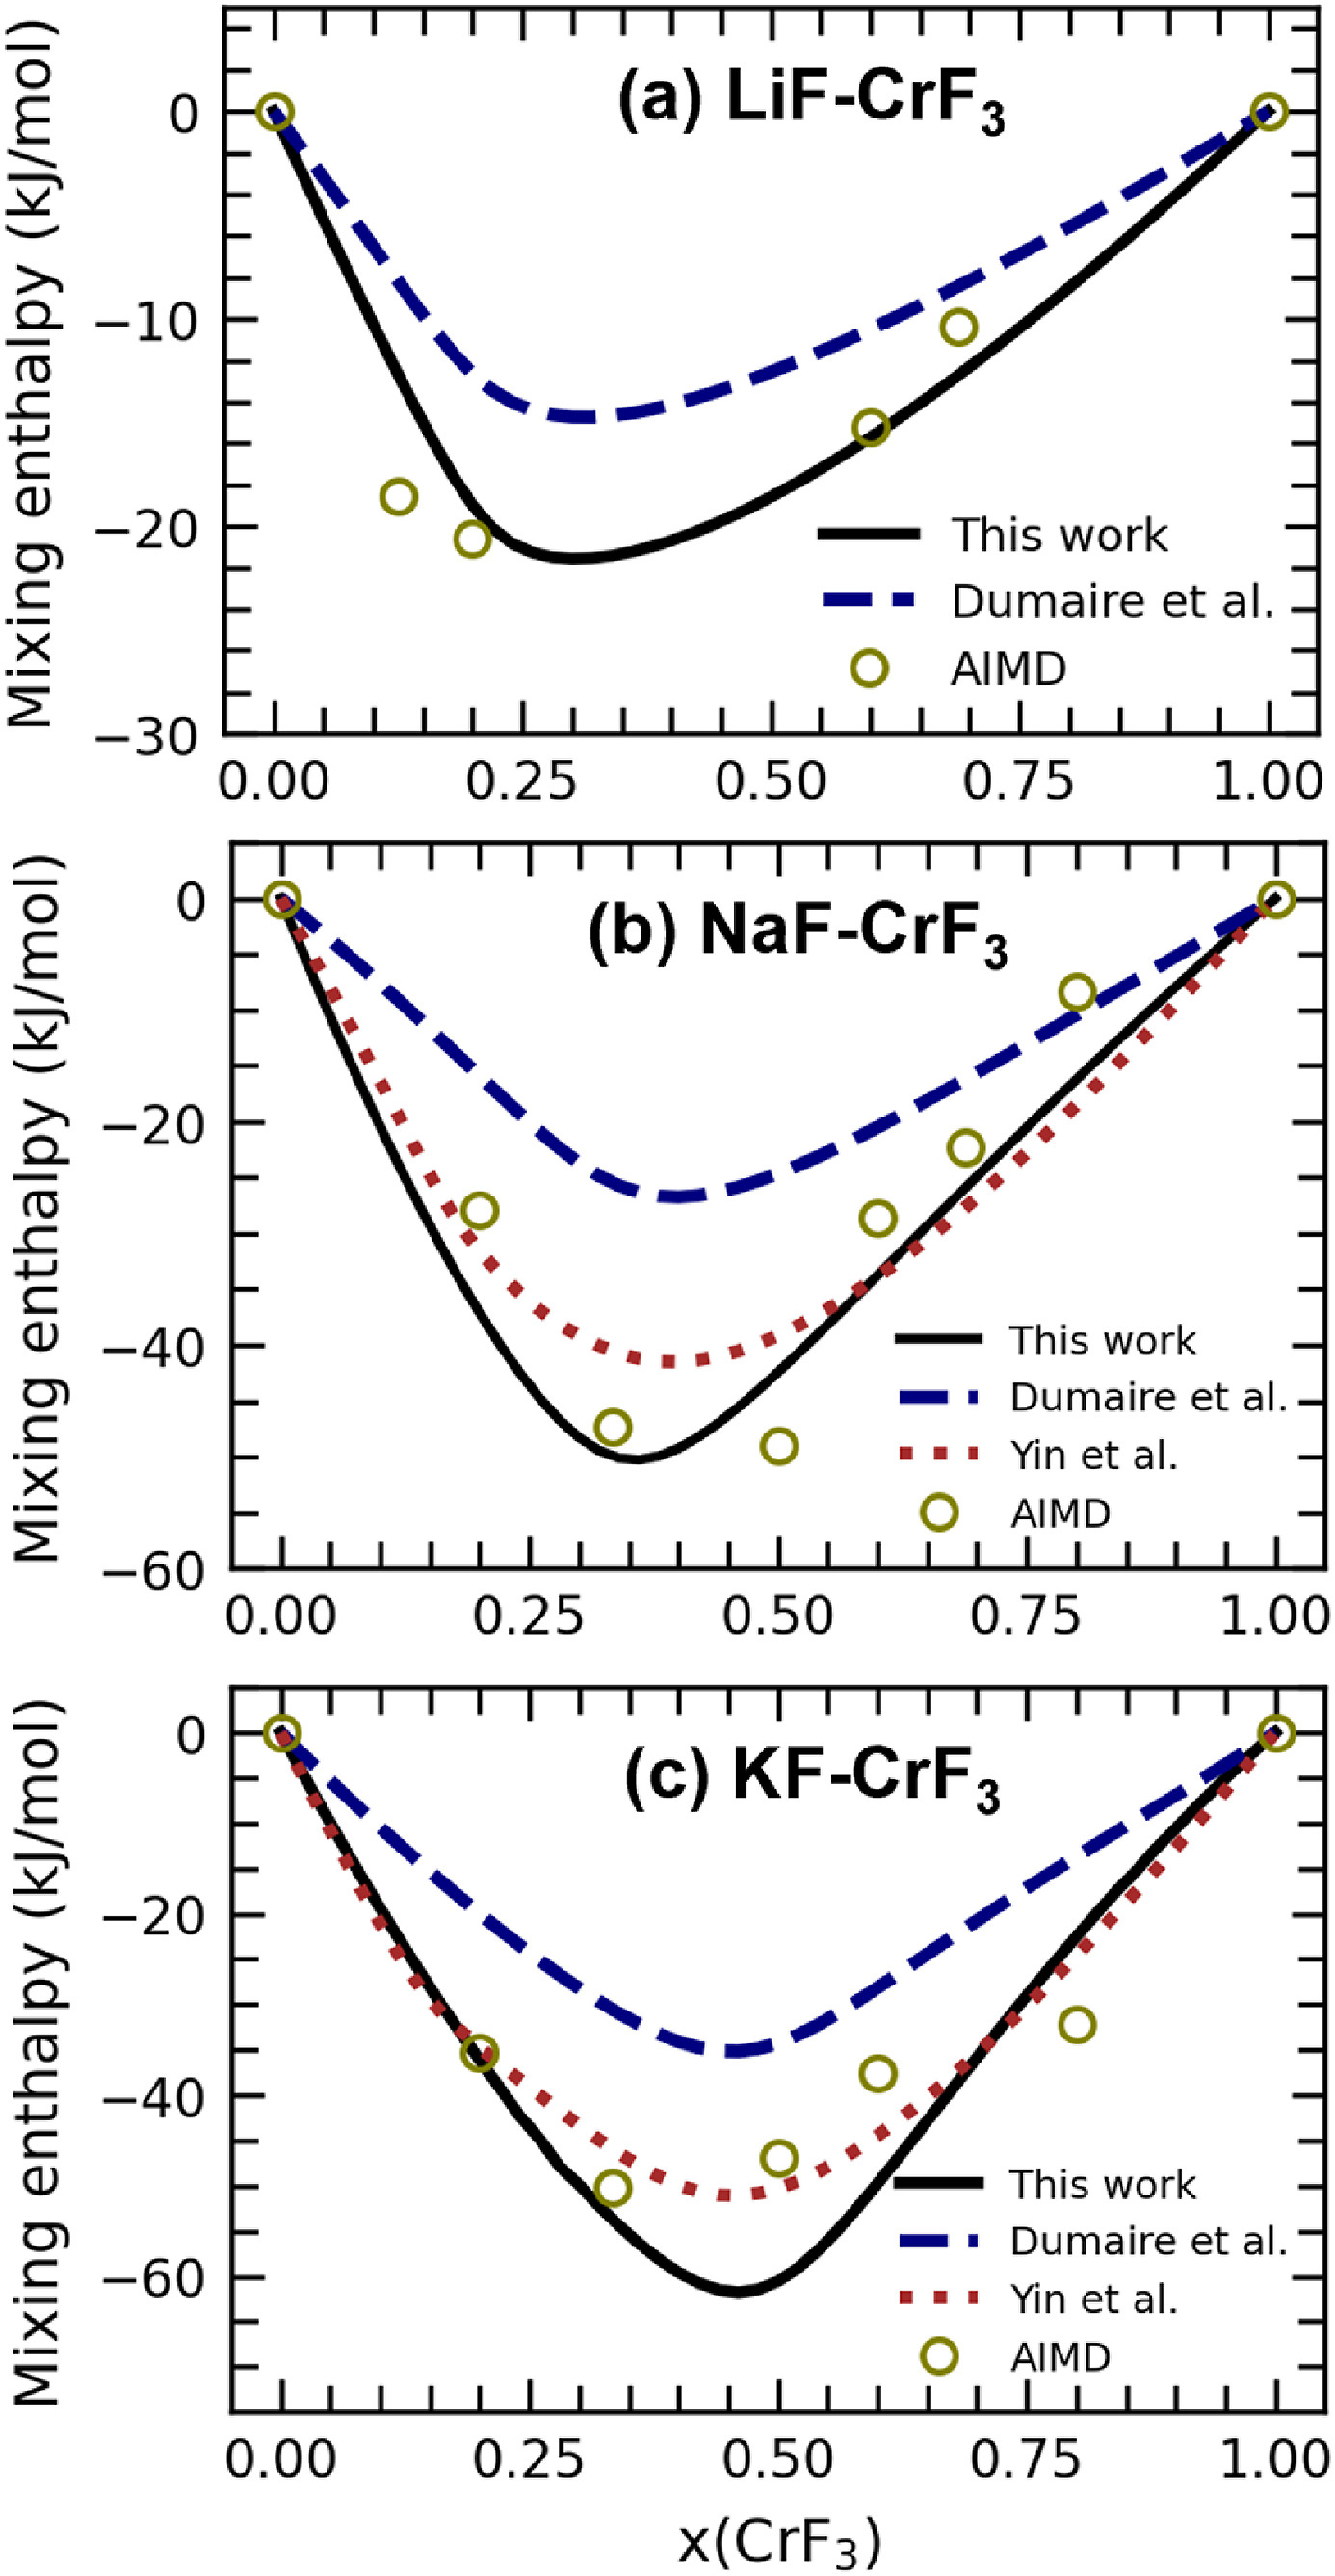
\includegraphics[width=0.45\linewidth]{moltensalts/Moltensalts-FLiNaKCr-Hmix.jpg}
    \caption{Predicted mixing enthalpy of liquid at 1700 K in (a) LiF-CrF$_3$, (b) NaF-CrF$_3$, and (c) KF-CrF$_3$ by the present CALPHAD modeling work (black solid lines), compared with the present AIMD results (circles) and modeling results by Dumaire et al. (blue dashed lines) \cite{dumaire2021thermodynamic} and Yin et al. (brown dotted lines) \cite{yin2018thermodynamic}.}
    \label{ms:fig:FLiNaKCr-Hmix}
\end{figure}

\begin{figure}[H]
    \centering
    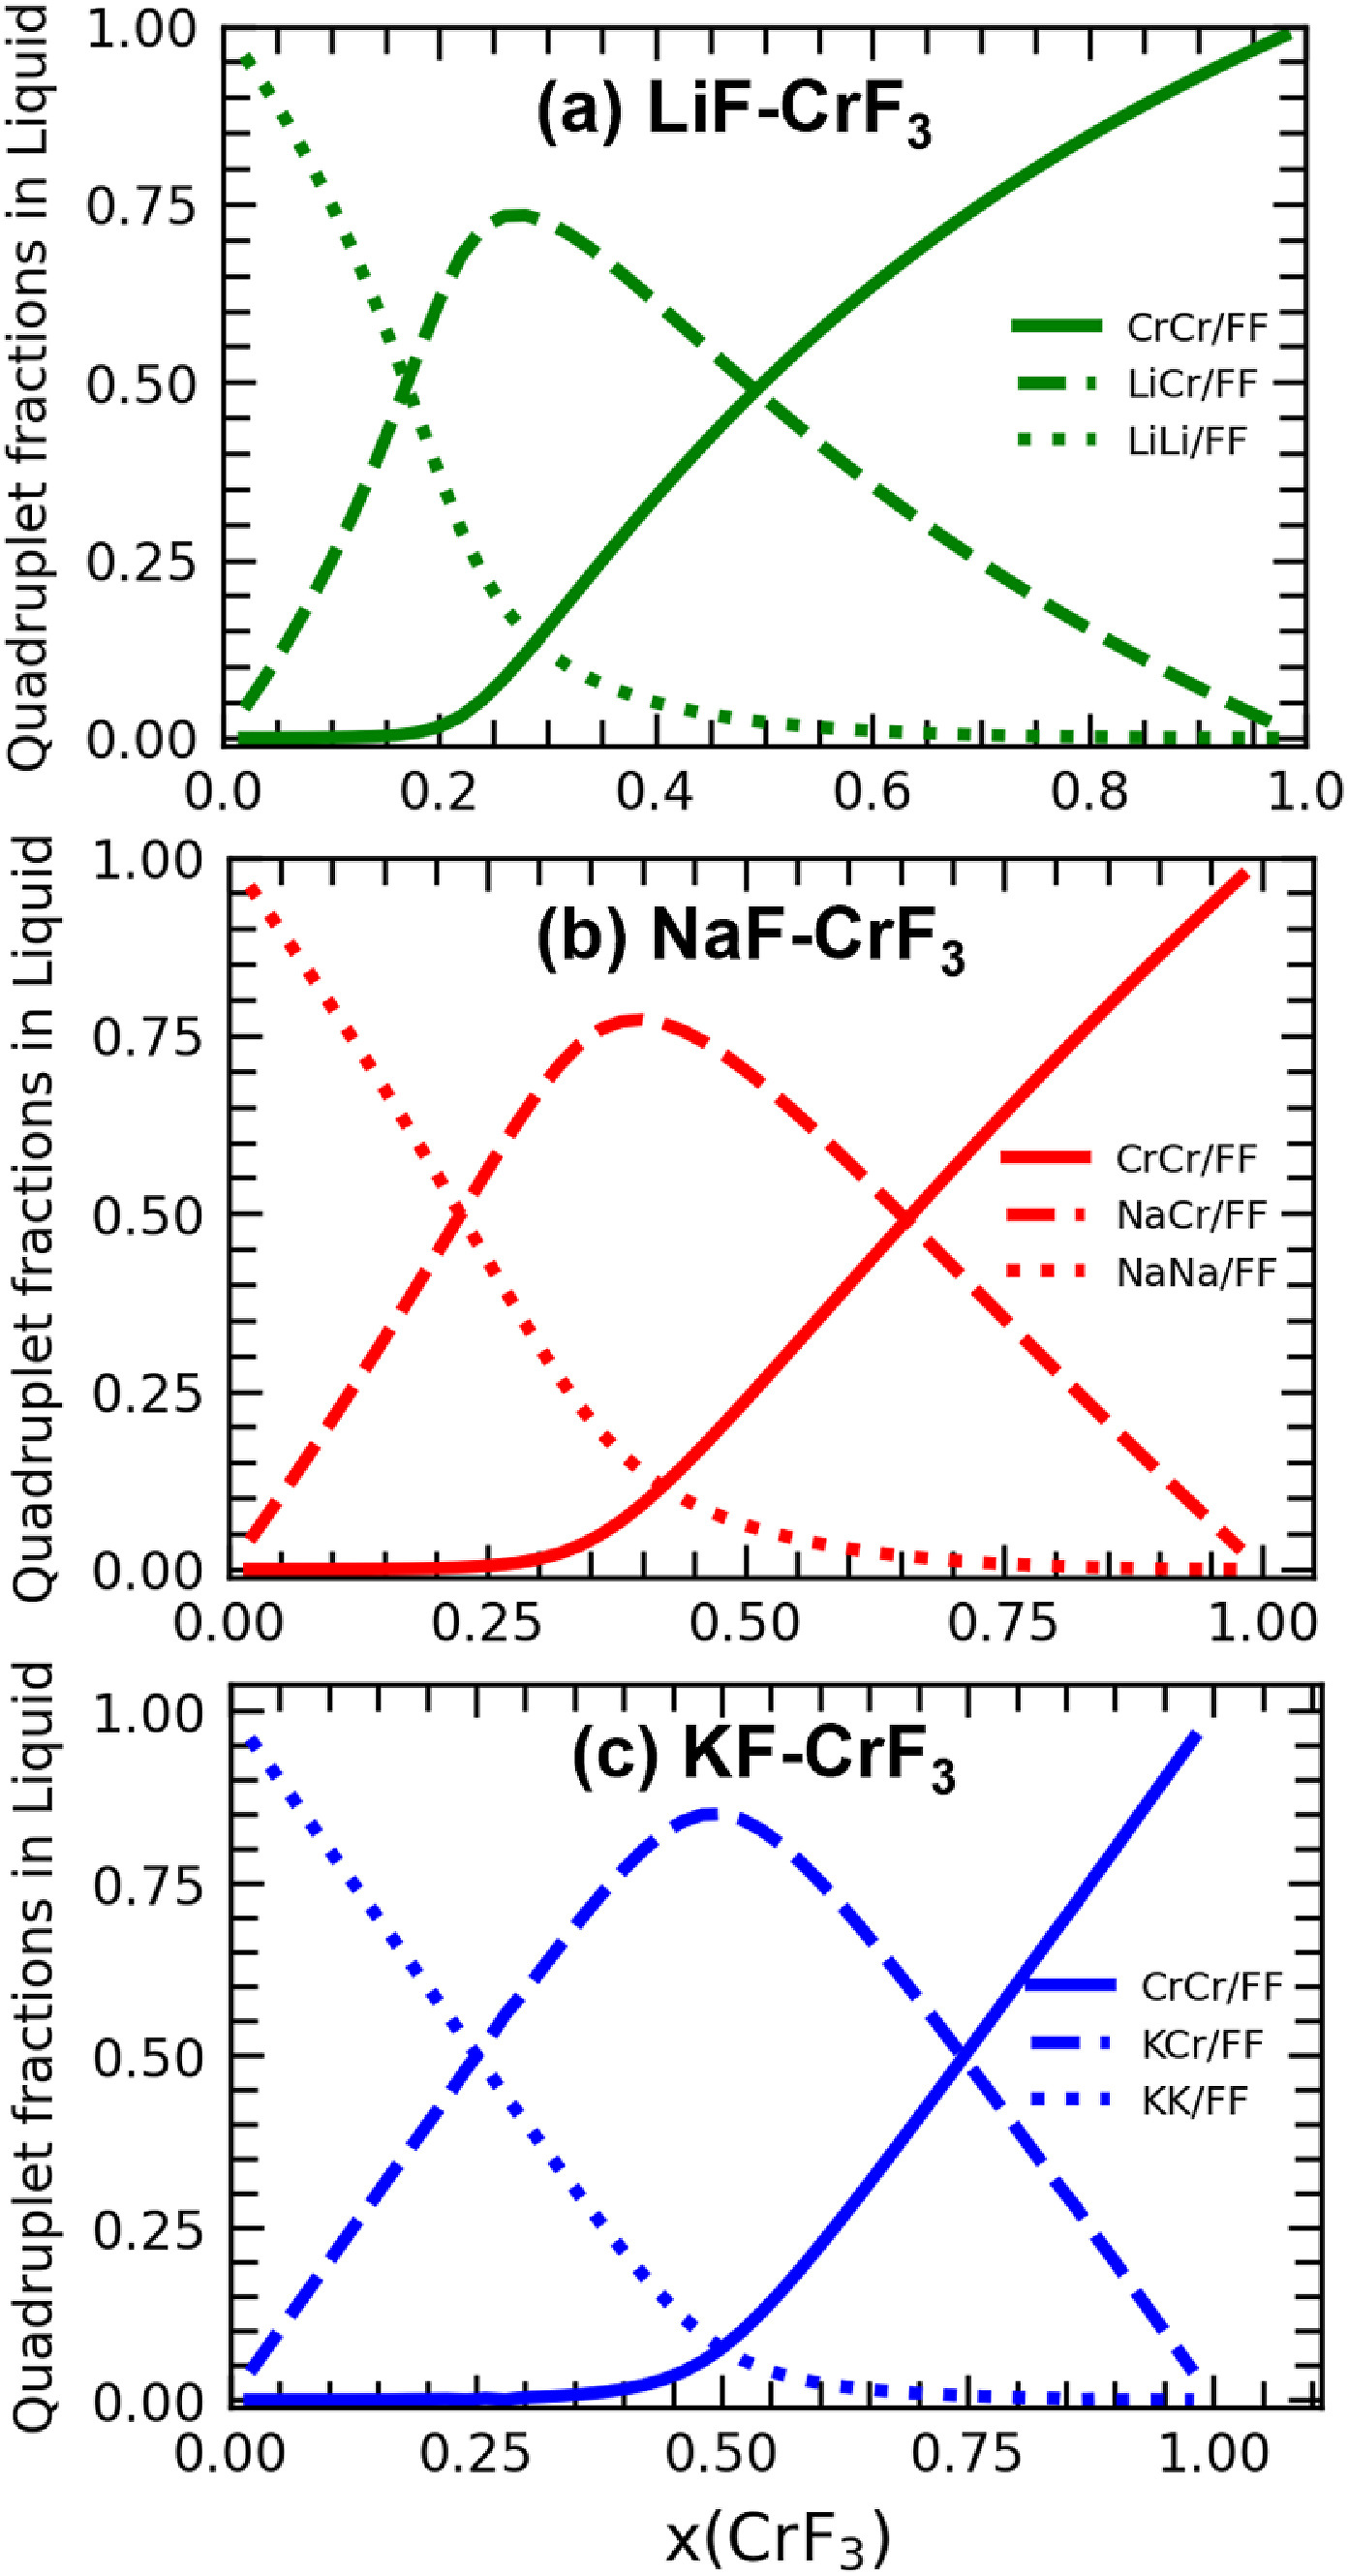
\includegraphics[width=0.45\linewidth]{moltensalts/Moltensalts-FLiNaKCr-QuadFrac.jpg}
    \caption{Precited quadruplet fractions in (a) LiF-CrF$_3$ (green lines), (b) NaF-CrF$_3$ (red lines), and (c) KF-CrF$_3$ (blue lines) liquid at 1700 K according to the present CALPHAD modeling. }
    \label{ms:fig:FLiNaKCr-QuadFrac}
\end{figure}

In Yin et al.’s modeling work \cite{yin2018thermodynamic}, the associate model was used to describe the liquid phase. This model was applied to describe the short-range ordering (SRO) by assuming ‘associates’, such as K$_3$CrF$_6$ and Na$_3$CrF$_6$ associates. This kind of assumption may cause issues when extrapolation into higher-order systems \cite{pelton2018phase}. In the present work, the MQMQA was employed to describe liquid and provide information on the first and the second nearest neighbors in complex liquid. As an example, Figure \ref{ms:fig:FLiNaKCr-QuadFrac} shows the predicted fraction of each quadruplet in the liquid phase. The composition where the peak fraction of the ACr/FF (A=Li, Na, and K) quadruplets appears, indicates the SRO. In the LiF-CrF$_3$ system, the peak fraction of LiCr:FF with strong SRO is around $x$(CrF$_3$) = 0.25, which is consistent with the lowest mixing enthalpy around the $x$(CrF$_3$) = 0.25 as shown in Figure \ref{ms:fig:FLiNaKCr-Hmix}. In addition, Figure \ref{ms:fig:FLiNaKCr-QuadFrac} presents the quadruplet fractions and the neighboring environments of ions in liquid, which are difficult to obtain from the associate model due to its focus on associate clusters.

\section{Bayesian model selection in thermodynamic modeling of LiCl-KCl-LaCl${_3}$} \label{moltensalts:sec:LaCl3}
In the CALPHAD community, several thermodynamic models, including the associate model, the two-sublattice ionic model, and the MQMQA, have been utilized to capture the complexity of molten salts. In the present work, the Bayes factor is used to guide the model selection process for thermodynamic modeling of the KCl-LaCl$_3$ system and provide statistical comparisons of various models. The results indicate that the MQMQA model is the most favorable based on available thermochemical data. The LiCl-KCl-LaCl$_3$ system has been further modeled with uncertainty quantification using MQMQA. Thermodynamic properties as a function of temperature for the compounds in KCl-LaCl$_3$ are predicted by the quasiharmonic approach in terms of first-principles phonon calculations. The calculated phase stability shows excellent agreement with experimental data, indicating that an appropriate thermodynamic model is important for accurately predicting the critical characteristics of complex molten salts.

The LiCl-KCl-LaCl$_3$ system contains the liquid phase, three binary compounds of LiCl, KCl, and LaCl$_3$, and two ternary compounds of K$_2$LaCl$_5$ and K$_3$La$_5$Cl$_{18}$ as summarized by Hao et al. \cite{hao2024thermodynamic}. K$_2$LaCl$_5$ was reported with a Pnma structure measured by Meyer et al. \cite{meyer1983k2mcl5}. Seifert et al. \cite{seifert1985thermodynamic} determined the structure of K$_3$La$_5$Cl$_{18}$ with a space group of $P6_3/m$ through X-ray diffraction. The values of formation enthalpy of K$_2$LaCl$_5$ and K$_3$La$_5$Cl$_{18}$ were measured by Seifert et al. \cite{seifert1985thermodynamic} using solution calorimetry. Reuter and Seifert \cite{reuter1994heat} reported the heat capacity values of K$_2$LaCl$_5$ and K$_3$La$_5$Cl$_{18}$ using differential scanning calorimetry (DSC). Gaune-Escard and Rycerz \cite{gaune1999heat} also measured the heat capacity of K$_3$La$_5$Cl$_{18}$ using DSC. Papatheodorou and Ostvold \cite{papatheodorou1974thermodynamic} reported mixing enthalpy in KCl-LaCl$_3$ through calorimetric experiments. Qiao et al. \cite{qiao1989measurement} utilized the differential thermal analysis (DTA) techniques to determine melting and phase transition temperatures. In the KCl-LaCl$_3$ system, Song and Zheng \cite{song1995investigation} measured liquidus by DTA. Seifert et al. \cite{seifert1985thermodynamic} measured phase boundaries in the LaCl$_3$-rich range by DTA.

In the ternary LiCl-KCl-LaCl$_3$ system, Bagri and Simpson \cite{bagri2016determination} and Samin et al. \cite{samin2016estimation} reported activity values for LaCl$_3$ in molten LiCl-KCl eutectic salt using electromotive force measurements and cyclic voltammetry, respectively. Regarding the phase diagram, Song and Zheng \cite{song1995investigation} reported the liquidus projection and six isopleths. Two research works, by Nakamura et al. \cite{nakamura1997thermal} and Venkata Krishnan et al. \cite{venkata2006pseudo}, constructed the pseudo-binary phase diagram from the LiCl-KCl eutectic to 25 mol\% of LaCl$_3$ in the LiCl-KCl eutectic through DSC.

\subsection{Modeling details} \label{moltensalts:ssec:LaCl3model}
Four frequently used models to describe complex molten salts are considered for the liquid phase in the KCl-LaCl$_3$, including the associate model \cite{sommer1982association}, the two-sublattice ionic model \cite{hillert1985two}, and the MQMQA \cite{pelton2001modified} (two sets of coordination numbers). 

The species KCl and LaCl$_3$ are assumed using the associate model \cite{sommer1982association} since no observation of other complex associates exists in the literature. The Gibbs energy of liquid can be expressed as: 
\begin{equation} \label{ms:eq:laassmG}
    \begin{aligned}
        G_m&=y_{\rm KCl}{{^o}G}_{\rm KCl}^{\rm Liquid}+y_{\rm {LaCl}_3}{{^o}G}_{\rm {LaCl}_3}^{Liquid}+RT\left(y_{KCl}\ln y_{\rm KCl}+y_{\rm {LaCl}_3}\ln y_{\rm {LaCl}_3}\right)\\&+y_{\rm KCl}y_{\rm {LaCl}_3}\sum_{v=0}{L_{\rm KCl,\rm {LaCl}_3}^v{(y_{\rm KCl}-y_{\rm {LaCl}_3})}^v}
    \end{aligned}
\end{equation}
where $y_i$ is the mole fraction of species $i$ (= KCl or LaCl$_3$), ${{^o}G}_i^{Liquid}$ the Gibbs energy of species $i$, $R$ the gas constant, and $L_{\rm KCl,{LaCl}_3}^v$ the $v^{th}$ interaction parameter, which can be expanded as in (\ref{method:eq:CEFLT}).

Using the two-sublattice ionic model \cite{hillert1985two}, the liquid phase in KCl-LaCl$_3$ can be described as: 
\begin{equation} \label{ms:eq:laionic}
    {({\rm K}^+,{\rm La}^{3+})}_P{({\rm Cl}^-)}_Q
\end{equation}
where the cations and anions are separated into two sublattices. The site ratios of $P$ and $Q$ follow the following relationships to maintain charge neutrality: 
\begin{equation} \label{ms:eq:laionicP}
    P=y_{{\rm Cl}^-}=1
\end{equation}
\begin{equation} \label{ms:eq:laionicQ}
    Q=y_{\rm K^+}+y_{{\rm La}^{3+}}
\end{equation}
where $y_i$ represents the mole fraction of ion $i$. The Gibbs energy function according to (\ref{method:eq:ionicGsrf}) and (\ref{method:eq:ionicScnf}) can be expressed as: 
\begin{equation} \label{ms:eq:laionicGm}
    G_m=y_{\rm K^+}{{^o}G}_{\rm KCl}^{Liquid}+y_{{\rm La}^{3+}}{{^o}G}_{{\rm LaCl}_3}^{Liquid}+RT\left(y_{\rm K^+}\ln y_{\rm K^+}+y_{{\rm La}^{3+}}lny_{{\rm La}^{3+}}\right)+{{^{xs}}G}_m 
\end{equation}
where ${{^{xs}}G}_m$ represents the excess Gibbs energy, which can be described based on the Redlich-Kister polynomial \cite{redlich1948algebraic} as described in (\ref{method:eq:ionicGxs}):
\begin{equation} \label{ms:eq:laionicGxs}
    {{^{xs}}G}_m=y_{\rm K^+}y_{{\rm La}^{3+}}\sum_{v=0}{L_{\rm K^+,{\rm La}^{3+}:{\rm Cl}^-}^v{(y_{K^+}-y_{{\rm La}^{3+}})}^v}
\end{equation}
where $L_{\rm K^+,{\rm La}^{3+}:{\rm Cl}^-}^v$ is the $v^{th}$ interaction parameter which can be described as in (\ref{method:eq:CEFLT}).

The MQMQA \cite{pelton2001modified} describes the KCl-LaCl$_3$ liquid phase by assuming interactions between the quadruplets of $\rm K_2{\rm Cl}_2$, ${\rm La}_2{\rm Cl}_2$, and ${\rm KLa}{\rm Cl}_2$. Coordination numbers $Z$ are defined to describe the second nearest neighbor coordination number of the species $i$ (= K, La, or Cl) in the quadruplets. $Z$ of anions can be calculated according to (\ref{method:eq:mqmqaZ}) to maintain charge neutrality. Coordination numbers used in the present work are summarized in Table \ref{ms:tab:lamqmZ}, where two sets of coordination numbers were applied to ${\rm KLa}{\rm Cl}_2$. The selection of MQMQA-M3 is based on Sun et al.’s modeling for KCl-NdCl$_3$ \cite{sun2004optimization}, while the MQMQA-M4 is based on the MSTDB-TC for KCl-LaCl$_3$ \cite{ard2022development}.

\begin{table}[H]
    \caption{Coordination numbers used in the present CALPHAD modeling with MQMQA for the liquid phase.}
    \centering
    \begin{tabular}{>{\raggedright\arraybackslash}m{1.5cm}>{\raggedright\arraybackslash}m{1.5cm}>{\raggedright\arraybackslash}m{3.5cm}>{\raggedright\arraybackslash}m{2.5cm}>{\raggedright\arraybackslash}m{2.5cm}>{\raggedright\arraybackslash}m{2.5cm}}
    \hline
    \textbf{A}&\textbf{B}&&$Z_{\rm AB:ClCl}^{\rm A}$&$Z_{\rm AB:ClCl}^{\rm B}$&$Z_{\rm AB:ClCl}^{\rm F}$ \\
    \hline
    K$^+$&K$^+$&&6.0&6.0&6.0\\
    La$^{3+}$&La$^{3+}$&&6.0&6.0&2.0\\
    K$^+$&La$^{3+}$&MQMQA-M3&2.0&6.0&2.0\\
    &&MQMQA-M4&3.5&6.0&2.55\\
    \hline
    \end{tabular}
    \label{ms:tab:lamqmZ}
\end{table}

The excess Gibbs energy is related to the formation Gibbs energy of the quadruplets as discussed in (\ref{method:eq:mqmqareac}). In the KCl-LaCl$_3$ system, this can be expressed as:
\begin{equation} \label{ms:eq:lamqmreac}
    \left(\rm K_2{\rm Cl}_2\right)_{quad}+\left({\rm La}_2{\rm Cl}_2\right)_{quad}=2\left(\rm KLa{\rm Cl}_2\right)_{quad}\;\;\;\;\Delta g_{\rm AB:Cl_2}^{ex}
\end{equation}
where $\Delta g_{\rm AB:Cl_2}^{ex}$ represents the Gibbs energy change when forming the quadruplets and can be described by: 
\begin{equation} \label{ms:eq:lamqmgex}
    \Delta g_{\rm AB:Cl_2}^{ex}=\Delta g_{\rm AB:Cl_2}^{o}+\sum_{(i+j)\geq1}{g_{\rm KLa:{\rm Cl}_2}^{ij}\chi_{\rm KLa:{\rm Cl}_2}^i\chi_{\rm LaK:{\rm Cl}_2}^j}
\end{equation}
where $g_{\rm KLa/{\rm Cl}_2}^{ij}$is a function of temperature and independent of composition. $\chi_{\rm KLa/{\rm Cl}_2}^i$ and $\chi_{\rm LaK/{\rm Cl}_2}^j$ are composition-dependent terms, defined as:
\begin{equation} \label{ms:eq:lamqmchi}
    \chi_{\rm KLa/{\rm Cl}_2}^i=\frac{X_{\rm K_2:Cl_2}}{X_{\rm K_2:Cl_2}+X_{\rm KLa:Cl_2}+X_{{\rm La}_2:{\rm Cl}_2}}
\end{equation}
where $X_{\rm KLa:Cl_2}$ is the fraction of $\left(\rm KLaCl_2\right)_{quad}$. 

All model parameters in the present work were optimized through the Bayesian approach using the MCMC method as implemented in ESPEI \cite{bocklund2019espei}. Each model parameter employed two Markov chains with a standard derivation of 0.1 when initializing its Gaussian distribution. During the modeling process, the chain values can be tracked and the MCMC processes were performed until the model parameters converged. The input data included primarily experimental phase equilibrium data for two or more co-existing phases, mixing enthalpy data, and activity data from the literature. For stochiometric compounds, their thermochemical data from DFT-based calculations were also used as input. 

The ternary compounds in the KCl-LaCl$_3$ system are considered stoichiometric compounds, including K$_2$LaCl$_5$ and K$_3$La$_5$Cl$_{18}$. Thermodynamic functions of the binary endmembers KCl and LaCl$_3$ are sourced from the JANAF tables \cite{chase1982janaf} and the SSUB database \cite{sgteurl}. The Gibbs energy for a given compound is expressed as in (\ref{ms:eq:Gstoi}). For these ternary compounds, their thermodynamic data including enthalpy, entropy, and heat capacity are obtained through DFT-based first-principles and phonon calculations. All DFT-based first-principles and phonon calculations in the present work were performed by the VASP \cite{kresse1996efficient}. The plane-wave basis cutoff energy was 262 eV for structural relaxations and 520 eV for the final static calculations of total energy. The convergent criterion of electronic self-consistency was set as $5\times10^{−6}$ eV/atom for relaxations and static calculations. Seifert et al. \cite{seifert1985thermodynamic} reported that K$_3$La$_5$Cl$_{18}$ possesses the symmetry of $P6_3/m$ with three Wyckoff sites of 2b, 2c, and 6h. However, the occupancy of the 2b site is less than 1, while the 2c site is occupied by both K and La atoms. Considering these, ATAT \cite{van2009multicomponent} was used to search for all possible configurations under these conditions, and 9 symmetry inequivalent configurations were found in terms of a 26-atom unit cell. The configuration with the lowest energy was predicted using DFT calculations. Phonon calculations were performed using the supercell method. Table \ref{ms:tab:ladftsetting} provides detailed settings for DFT-based first-principles and phonon calculations, including reciprocal k-points meshes and supercell sizes for phonon calculations, which ensures the convergence and accuracy of the DFT calculations.

\begin{table}[H]
    \caption{Details of the present DFT-based first-principles and phonon calculations for each compound, including space group, total atoms in the supercells, k-point meshes for structure relaxations, and the final static calculations (indicated by DFT), supercell sizes for phonon calculations, and k-point meshes for phonon calculations.}
    \centering
    \begin{tabular}{>{\raggedright\arraybackslash}m{2cm}>{\raggedright\arraybackslash}m{2cm}>{\raggedright\arraybackslash}m{3.5cm}>{\raggedright\arraybackslash}m{2.5cm}>{\raggedright\arraybackslash}m{2.5cm}>{\raggedright\arraybackslash}m{2.5cm}}
    \hline
    \textbf{Phase}&\textbf{Space Group}&\textbf{Atoms in crystallographic cell}&\textbf{k-points for DFT}&\textbf{Atoms in supercell for phonon}&\textbf{k-points for phonon}\\
    \hline
    KCl&$Fm\bar{3}m$&8&$8\times8\times8$&64&$3\times3\times3$\\
    LaCl$_3$&$P6_3/m$&8&$8\times8\times12$&64&$2\times2\times2$\\
    K$_2$LaCl$_5$&$Pnma$&32&$7\times7\times4$&32&$4\times4\times2$\\
    K$_3$La$_5$Cl$_{18}$&$P3$&26&$8\times8\times5$&26&$5\times5\times3$\\
    \hline
    \end{tabular}
    \label{ms:tab:ladftsetting}
\end{table}

\subsection{Thermodynamic properties in LiCl-KCl-LaCl$_3$ by first-principles calculations} \label{moltensalts:ssec:LaCl3DFTresult}
Thermodynamic properties of compounds in the KCl-LaCl$_3$ system were predicted using first-principles calculations. Table \ref{ms:tab:lacl3eosresults} summarizes the equilibrium properties of V$_0$, B$_0$, and B$^\prime$ at 0 K obtained by DFT-based calculations in comparison with experiments. The present work predicts the bulk modulus B$_0$ value to be 16.23 GPa for KCl, which is slightly lower than the experimental measurement of 19.7 GPa by Norwood et al. \cite{norwood1958elastic}. The equilibrium volume V$_0$ of LaCl$_3$ is predicted to be 27.37 \r{A}$^3$/atom in the present work, which is in good agreement with the measured 26.38 \r{A}$^3$/atom by Zachariasen \cite{Zachariasen1947}. It indicates that the present DFT calculations provide reliable predictions regarding the equilibrium properties of compounds in the KCl-LaCl$_3$ system. The present DFT calculations predicted the V$_0$ of K$_2$LaCl$_5$ to be 29.96 \r{A}$^3$/atom and B$_0$ to be 15.89 GPa. For K$_3$La$_5$Cl$_{18}$, the V$_0$ is reported to be 27.49 \r{A}$^3$/atom and B$_0$ to be 26.46 GPa.

\begin{table}[H]
    \caption{Predicted equilibrium properties of volume V$_0$, bulk modulus B$_0$, and the first derivative of bulk modulus with respect to pressure B$^\prime$ for compounds in the KCl-LaCl$_3$ system based on the present EOS fitting at 0 K. Experimental data are also listed for comparison.}
    \centering
    \begin{tabular}{>{\raggedright\arraybackslash}m{3cm}>{\raggedright\arraybackslash}m{3cm}>{\raggedright\arraybackslash}m{2.5cm}>{\raggedright\arraybackslash}m{2cm}>{\raggedright\arraybackslash}m{4cm}}
    \hline
    \textbf{Compounds}&\textbf{V$_0$}\ (\r{A}$^3$/atom)&\textbf{B$_0$}\ (GPa)&\textbf{B$^\prime$}&\textbf{Reference}\\
    \hline
    KCl&32.62&16.23&4.67&This work\\
    &&19.7&&Norwood et al. \cite{norwood1958elastic}\\
    LaCl$_3$&27.37&29.02&6.40&This work\\
	&26.38&&&Zachariasen \cite{Zachariasen1947}\\
    K$_2$LaCl$_5$&29.96&15.89&5.38&This work\\
    K$_3$La$_5$Cl$_{18}$&27.49&26.46&6.35&This work\\
    \hline
    \end{tabular}
    \label{ms:tab:lacl3eosresults}
\end{table}

Thermodynamic properties at finite temperatures are obtained through DFT-based QHA in terms of phonon. Figure \ref{ms:fig:lacl3pureQHA} compares the predicted values of heat capacity C$_p$, entropy $S$, and enthalpy $H-H_{300}$ of KCl and LaCl$_3$ to those from the SGTE database \cite{sgteurl}. For the KCl, the present QHA results align closely with the SGTE data \cite{sgteurl}, although the DFT values are slightly higher. The $S$ also shows a good agreement, with a minor difference of about 6\%. For the LaCl$_3$, the present QHA results slightly underpredict C$_p$ and $H-H_{300}$ compared to SGTE \cite{sgteurl}, particularly at higher temperatures. The differences in C$_p$ for LaCl$_3$ remain less than 3.2 J/mol-atom-K at high temperatures, while the entropy and enthalpy differences closely match the SGTE values \cite{sgteurl}. Figure \ref{ms:fig:lacl3CompoundsCp} shows the predicted heat capacities C$_p$ of K$_2$LaCl$_5$ and K$_3$La$_5$Cl$_{18}$ in comparison with experiments \cite{reuter1994heat, gaune1999heat}, demonstrating an excellent agreement. For example, at 500 K, QHA results show the K$_2$LaCl$_5$ C$_p$ of 26.99 J/mol-K, which is 0.8\% higher compared to 26.77 J/mol-K reported by Reuter et al. \cite{reuter1994heat} and 0.5\% higher than 26.86 J/mol-K by Gaune-Escard et al. \cite{gaune1999heat}. For K$_3$La$_5$Cl$_{18}$, the C$_p$ at 500 K is predicted to be 25.99 J/mol-K, slightly lower than 26.34 J/mol-K by Reuter et al. \cite{reuter1994heat}. These results of K$_2$LaCl$_5$ and K$_3$La$_5$Cl$_{18}$ obtained from the present DFT calculations are then used in the present CALPHAD modeling.

\begin{figure} [H]
    \centering
    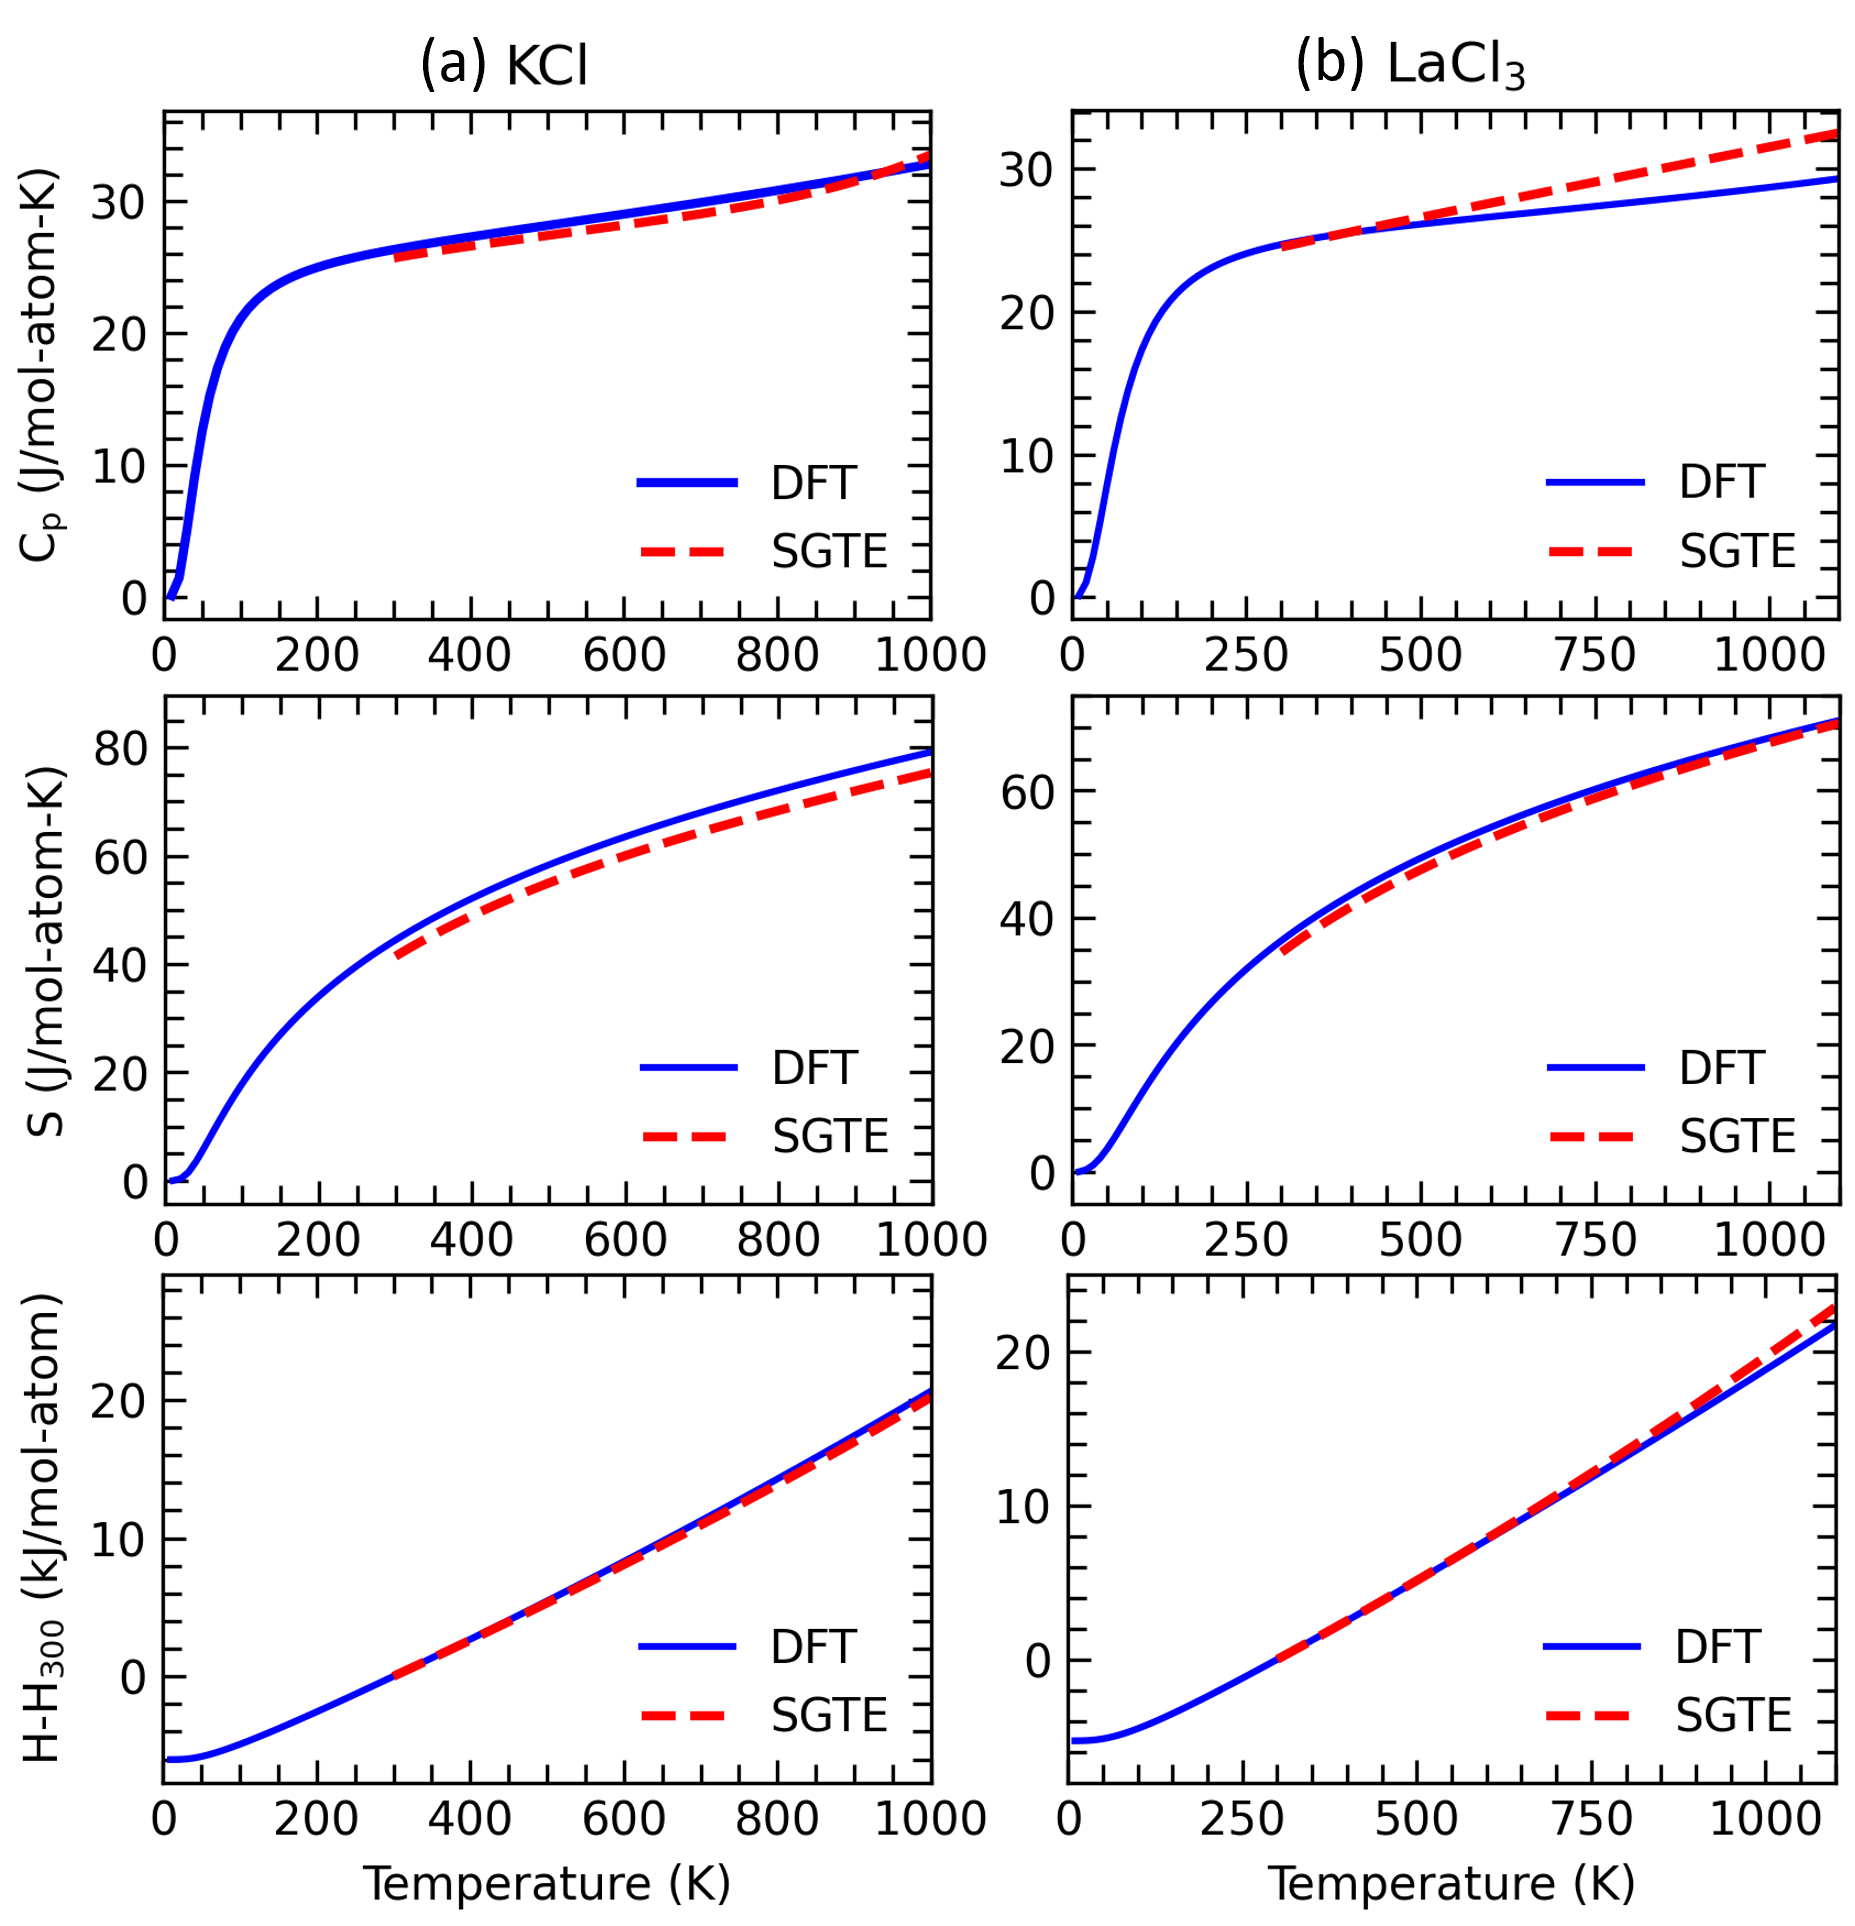
\includegraphics[width=0.9\linewidth]{moltensalts/Moltensalts-LaCl3-Cp-S-H.png}
    \caption{Comparison of the present values (blue lines) of heat capacity C$_p$, entropy $S$, and enthalpy with reference at 300 K ($H-H_{300}$) for (a) KCl and (b) LaCl$_3$ from the DFT-based phonon calculations (blue lines) with the SGTE data \cite{sgteurl} (red dash lines).}
    \label{ms:fig:lacl3pureQHA}
\end{figure}

\begin{figure} [H]
    \centering
    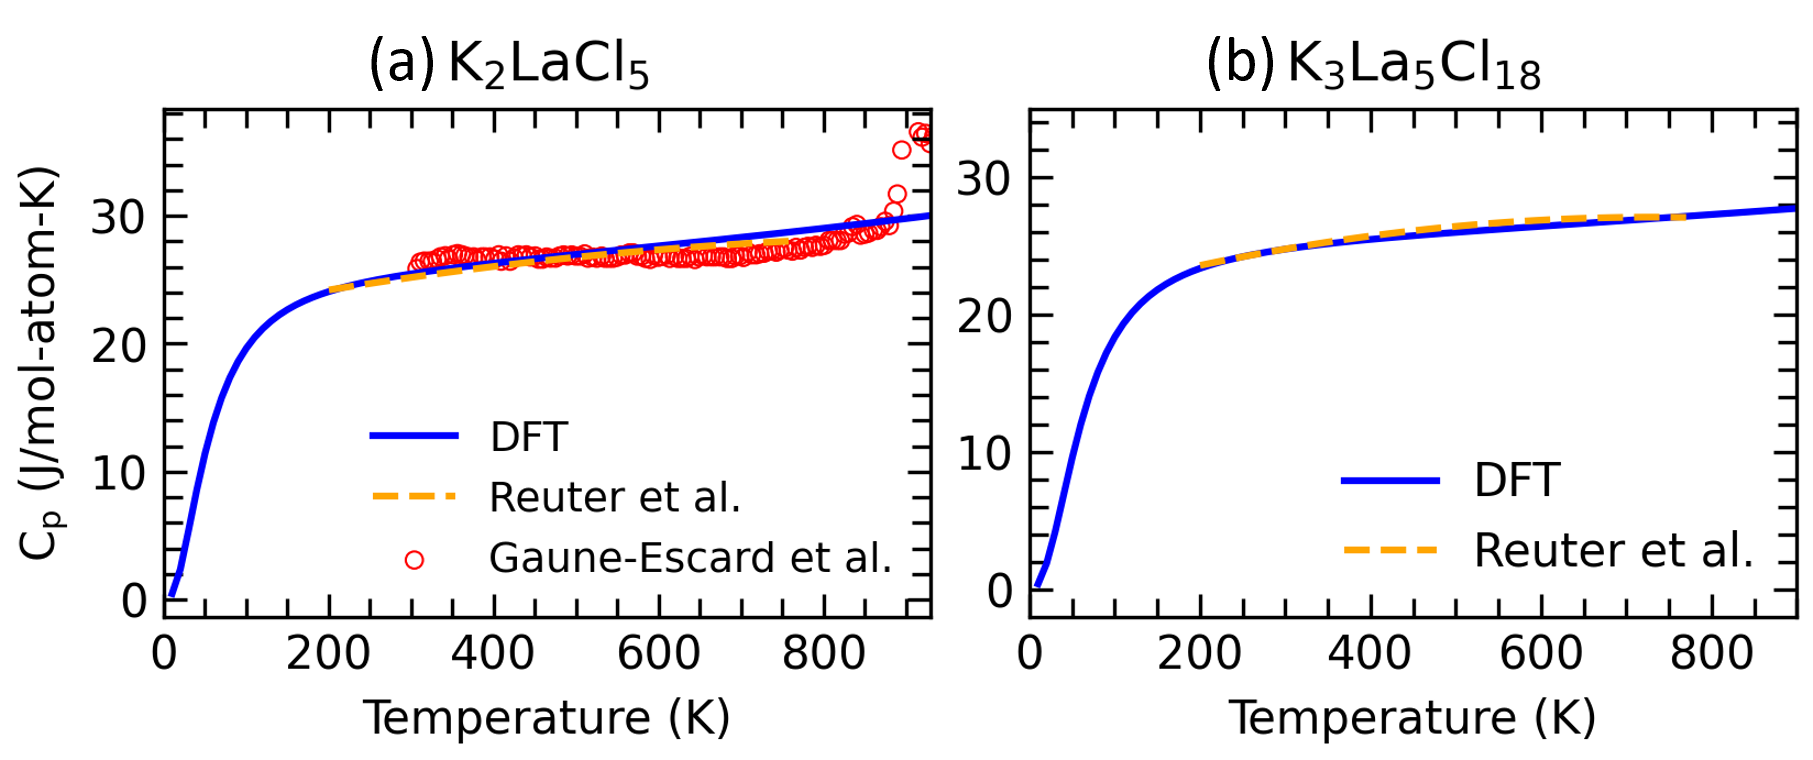
\includegraphics[width=0.9\linewidth]{moltensalts/Moltensalts-LaCl3-Compounds-Cp.png}
    \caption{Comparison of heat capacity C$_p$ values for (a) K$_2$LaCl$_5$ and (b) K$_3$La$_5$Cl$_{18}$ from the present DFT-based QHA (blue lines) with experiments by Reuter et al. \cite{reuter1994heat} (yellow dash lines) and Gaune-Escard et al. \cite{gaune1999heat} (red circles).}
    \label{ms:fig:lacl3CompoundsCp}
\end{figure}

\subsection{Model selection for the liquid phase in the KCl-LaCl$_3$ system} \label{moltensalts:ssec:LaCl3modelselection}
The KCl-LaC3 system is modeled using four models, the associate model (Associate-M1), the ionic model (Ionic-M2), and the MQMQA-M3 and the MQMQA-M4 with different coordination numbers as introduced in Section \ref{moltensalts:ssec:LaCl3model}. Experimental data are also listed for comparison. Each model has four adjustable parameters and was optimized by at least 1000 MCMC iterations. This process continued until the posterior probability values from each Markov chain stabilized, i.e., the model parameters converged. Figure \ref{ms:fig:lacl3PDfourm} compares the phase diagrams of these four models with experimental data \cite{seifert1985thermodynamic, song1995investigation}. It shows that for the liquidus of the KCl-rich region, MQMQA-M3 and MQMQA-M4 provide better agreements with experimental data than Associate-M1 and Ionic-M2. Table \ref{ms:tab:lacl3inv} lists the invariant reactions predicted by different models in comparison with experimental data \cite{seifert1985thermodynamic, song1995investigation}. All these four models show excellent agreement with the experimental data. Ionic-M2 and MQMQA-M4 slightly overpredict the invariant temperatures compared to those from Asscociate-M1 and MQMQA-M3. Specifically, Ionic-M2 and MQMQA-M4 predict a eutectic temperature of 854 K for the reaction of Liquid $\leftrightarrow$ KCl+K$_2$LaCl$_5$, which is 9 K higher than 845 K reported by Song et al. \cite{song1995investigation} and 1 K above 853 K by Seifert et al. \cite{seifert1985thermodynamic}. For the melting temperature of K$_2$LaCl$_5$, Ionic-M2 predicts 917 K, while MQMQA-M4 predicts 926 K, both are higher than the measured 913 K by Seifert et al. \cite{seifert1985thermodynamic} and 916 K by Song et al. \cite{song1995investigation}. Associate-M1 slightly underpredicts the peritectic temperature of the reaction Liquid+LaCl$_3$ $\leftrightarrow$ K$_3$La$_5$Cl$_{18}$ at 882 K, which is 3 K lower than the 885 K by Seifert et al. \cite{seifert1985thermodynamic} and the other models. The MAE for predicting these invariant temperatures using Associate-M1 is 2.5 K. MQMQA-M3 provides a good agreement with experimental data, with a slightly lower prediction of eutectic temperature for the reaction Liquid $\leftrightarrow $K$_2$LaCl$_5$+K$_3$La$_5$Cl$_{18}$ at 845 K, which is 6 K lower than 851 K reported by Seifert et al. \cite{seifert1985thermodynamic}. Regarding the invariant compositions $x$(LaCl$_3$), MQMQA-M3 and MQMQA-M4 offer better predictions with an MAE of 0.017 for both, compared to 0.025 for Associate-M1 and 0.022 for Ionic-M2. 

\begin{figure}[H]
    \centering
    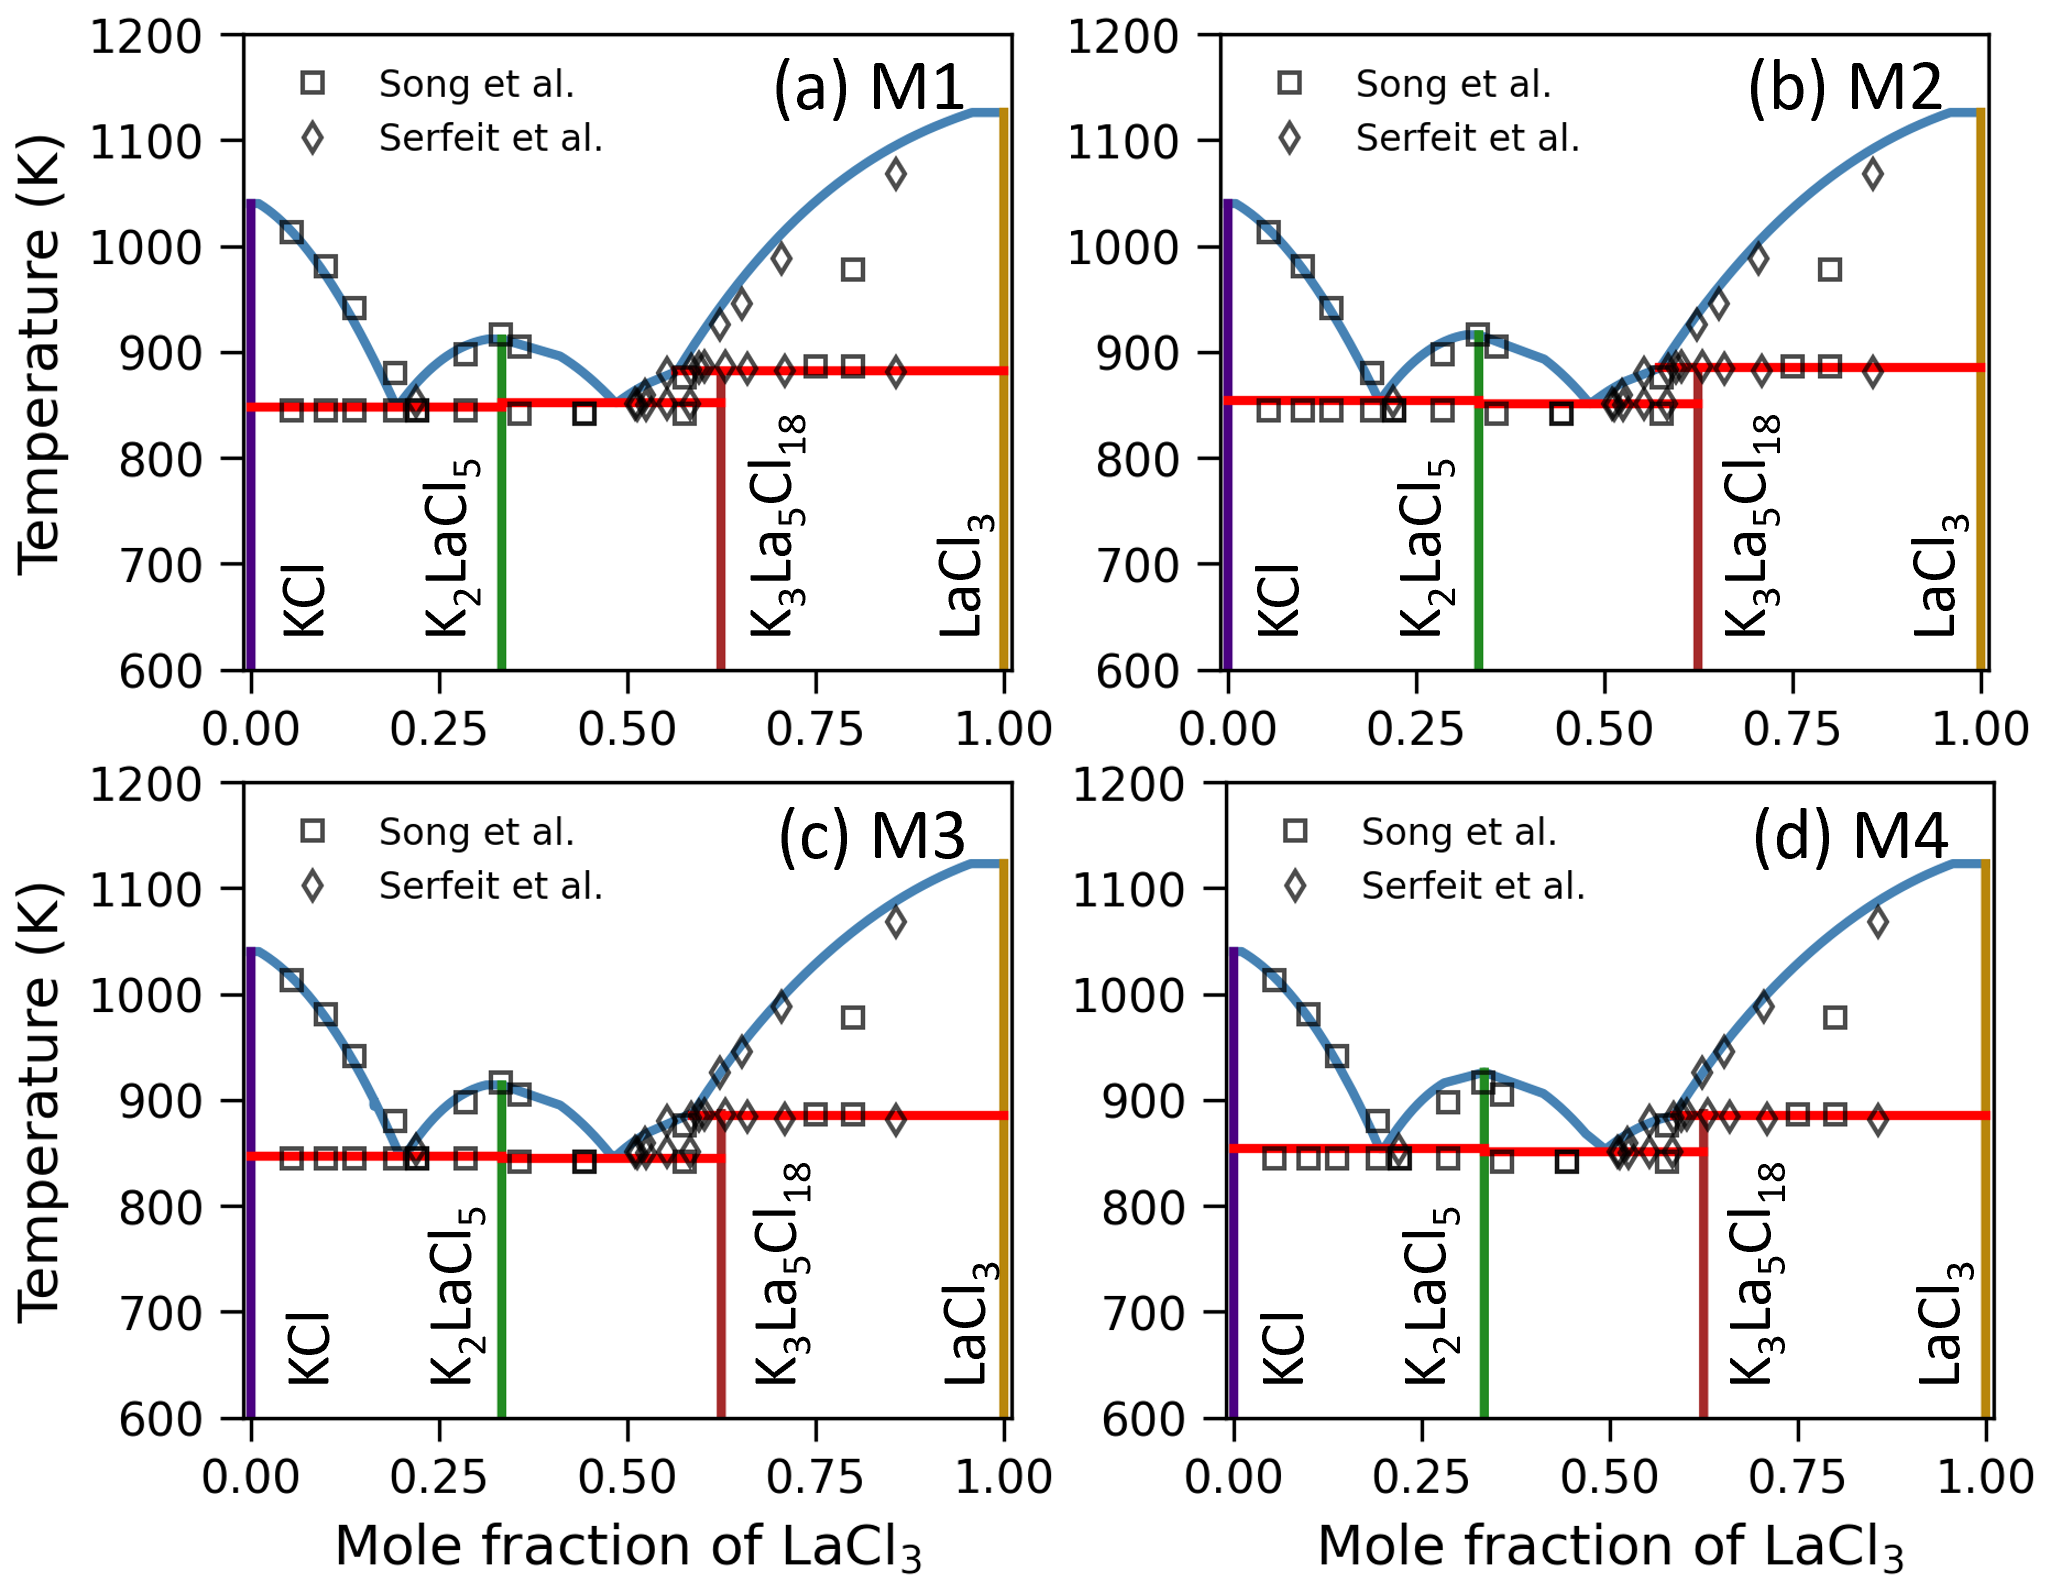
\includegraphics[width=0.9\linewidth]{moltensalts/Moltensalts-LaCl3-PhaseDiagram-Fourmodels-m.png}
    \caption{Predicted phase diagrams of the KCl-LaCl$_3$ system with the liquid phase modeled using (a) associate model (Associate-M1), (b) ionic model (Ionic-M2), (c) MQMQA (MQMQA-M3), and (d) MQMQA (MQMQA-M4) in comparison to experimental data \cite{seifert1985thermodynamic, song1995investigation}.}
    \label{ms:fig:lacl3PDfourm}
\end{figure}

\begin{table}[H]
    \caption{Predicted invariant equilibria in the KCl-LaCl$_3$ system by the four models, compared with experimental data.}
    \centering
    \begin{tabular}{>{\raggedright\arraybackslash}m{2cm}>{\raggedright\arraybackslash}m{5.5cm}>{\raggedright\arraybackslash}m{2cm}>{\raggedright\arraybackslash}m{2.5cm}>{\raggedright\arraybackslash}m{3.5cm}}
    \hline
    \textbf{Reaction}&&\textbf{$x$(LaCl$_3$)}&\textbf{Temperature} (K)&\textbf{Reference}\\
    \hline
    Eutectic&Liquid$\leftrightarrow$KCl+K$_2$LaCl$_5$&0.22&853&Seifert et al. \cite{seifert1985thermodynamic}\\
    &&0.22&845&Song et al. \cite{song1995investigation}\\
    &&0.197&848&Associate-M1\\
    &&0.202&854&Ionic-M2\\
    &&0.204&847&MQMQA-M3\\
    &&0.200&854&MQMQA-M4\\
    Melting&Liquid$\leftrightarrow$K$_2$LaCl$_5$&0.333&913&Seifert et al. \cite{seifert1985thermodynamic}\\
    &&0.333&916&Song et al. \cite{song1995investigation}\\
    &&0.333&913&Associate-M1\\
    &&0.333&917&Ionic-M2\\
    &&0.333&915&MQMQA-M3\\
    &&0.333&926&MQMQA-M4\\
    Eutectic&Liquid$\leftrightarrow$K$_2$LaCl$_5$+K$_3$La$_5$Cl$_{18}$&0.51&851&Seifert et al. \cite{seifert1985thermodynamic}\\
    &&0.485&852&Associate-M1\\
    &&0.481&851&Ionic-M2\\
    &&0.482&845&MQMQA-M3\\
    &&0.49&851&MQMQA-M4\\
    Peritectic&Liquid+LaCl$_3$$\leftrightarrow$K$_3$La$_5$Cl$_{18}$&0.595&885&Seifert et al. \cite{seifert1985thermodynamic}\\
    &&0.565&882&Associate-M1\\
    &&0.573&885&Ionic-M2\\
    &&0.586&885&MQMQA-M3\\
    &&0.586&885&MQMQA-M4\\
    \hline
    \end{tabular}
    \label{ms:tab:lacl3inv}
\end{table}

Figure \ref{ms:fig:lacl3HMRfourm} shows the values of mixing enthalpy of liquid at 1173 K calculated using these four models, compared with experimental data by Papatheodorou and Ostvold \cite{papatheodorou1974thermodynamic}. The comparison indicates that Associate-M1 and Ionic-M2 predict lower mixing enthalpy values than those by MQMQA-M3 and MQMQA-M4. For example, at $x$(LaCl$_3$) = 0.496, Associate-M1 predicts $-$15.469 kJ/mol and Ionic-M2 predicts $-$15.455 kJ/mol, slightly lower than the $-$15.097 kJ/mol predicted by MQMQA-M3 and $-$15.118 kJ/mol by MQMQA-M4. When compared to the mixing enthalpy value of $-$15.319 kJ/mol reported by Papatheodorou and Ostvold  \cite{papatheodorou1974thermodynamic}, Associate-M1 and Ionic-M2 show a closer alignment, with a difference of 0.9\%, compared to a 1.4\% difference for MQMQA-M3 and MQMQA-M4. Notably, Associate-M1 and Ionic-M2 align more closely with experimental data \cite{papatheodorou1974thermodynamic}, particularly in the composition region with $x$(LaCl$_3$) > 0.4. 

\begin{figure} [H]
    \centering
    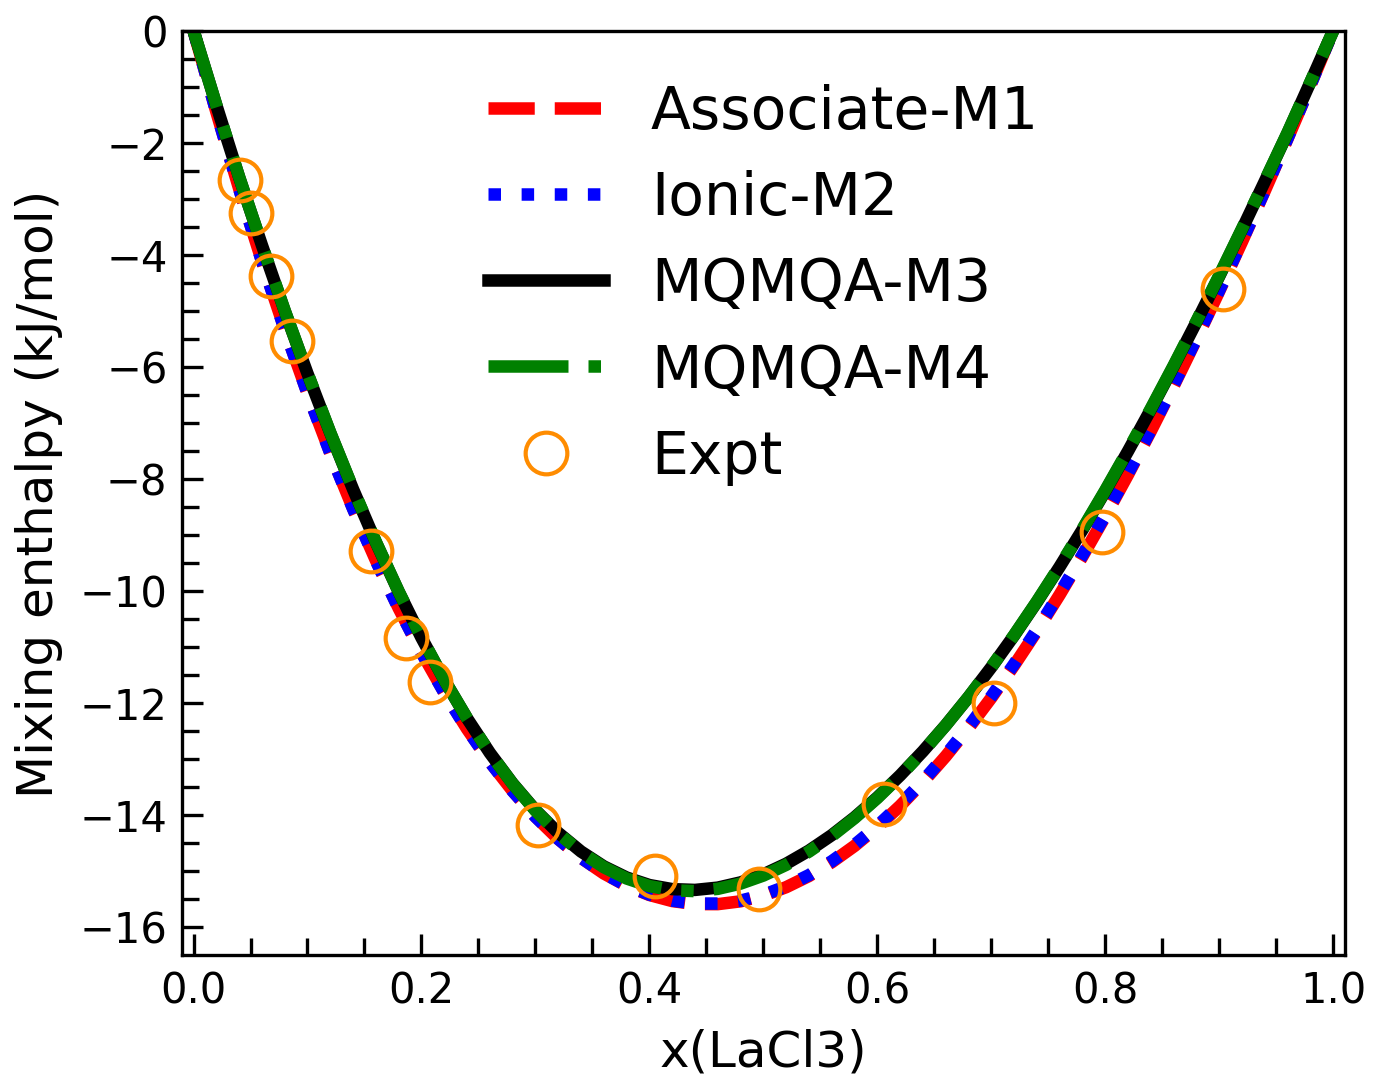
\includegraphics[width=0.5\linewidth]{moltensalts/Moltensalts-LaCl3-HMR-FourModels.png}
    \caption{Predicted values of mixing enthalpy of the KCl-LaCl$_3$ liquid at 1173K from four models in comparison with experimental data by Papatheodorou and Ostvold \cite{papatheodorou1974thermodynamic}. The red dash line represents Associate-M1, the blue dotted line represents Ionic-M2, the black solid line represents MQMQA-M3, and the green dash-dotted line represents MQMQA-M4.}
    \label{ms:fig:lacl3HMRfourm}
\end{figure}

According to phase diagrams (Figure \ref{ms:fig:lacl3PDfourm}) and mixing enthalpy predictions (Figure \ref{ms:fig:lacl3HMRfourm}), each model demonstrates a strength in predicting thermodynamic properties of the KCl-LaCl$_3$ system. Associate-M1 and Ionic-M2 perform well in predicting mixing enthalpy, showing a better match with experimental data as discussed above. However, these two models are less accurate in predicting phase boundaries compared to MQMQA-M3 and MQMQA-M4, especially in the LaCl$_3$-rich region. Choosing an appropriate model remains a challenge, as it requires balancing agreement with all available experimental data. A quantitative method is hence needed to determine the overall favorability for the models of study.

Bayesian parameter estimation through MCMC offers a powerful tool to statistically compare models, as demonstrated in Section \ref{method:ssec:Bayesian}. In the present work, the last 600 iterations from MCMC were used to compute the marginal likelihood $p\left(D\middle| M\right)$ for each model. Table \ref{ms:tab:lacl3bayesK} lists the estimated marginal likelihood value for each model, indicating that MQMQA-M3 has the highest marginal likelihood value of $\ln(p\left(D\middle| M_3\right))$ = $-370.628$. Consequently, the Bayes factors for the other models were calculated with respect to MQMQA-M3, using the marginal likelihood value of MQMQA-M3 as the numerator in (\ref{method:eq:BayesFactor}). The interpretation of the Bayes factor is also included in Table \ref{ms:tab:lacl3bayesK} according to the guideline by Kass and Raftery \cite{kass1995bayes}. That is, a ${log}_{10}({\rm Bayes factor})$ value between 0 and 1/2 suggests not worth more than a bare mention in comparing two models even if it points very slightly towards the model at the denominator, a range of 1/2 to 1 indicates substantial evidence in favor of the model at the denominator, 1 to 2 denotes strong evidence, and a value greater than 2 represents decisive evidence in favor of the model at the denominator. The present results indicate that the marginal likelihoods of Ionic-M2 $\ln(p\left(D\middle| M_2\right))$ = $-373.410$ and MQMQA-M4 $\ln(p\left(D\middle| M_4\right))$ = $-371.420$ are close to that of MQMQA-M3. In contrast, the marginal likelihood of Associate-M1 $\ln(p\left(D\middle| M_1\right))$ = $-439.135$ is significantly lower than that of MQMQA-M3, indicating that the Associate-M1 model is less favorable compared to the other three models. The Bayes factor ${log}_{10}K_{M3/M1}$ is 29.752, suggesting decisive evidence of favoring MQMQA-M3 over Associate-M1. This is due to the larger discrepancy in phase boundary predictions from Associate-M1 compared to the experimental phase diagram data shown in Figure \ref{ms:fig:lacl3PDfourm}(a). Regarding the Ionic-M2, the Bayes factor ${log}_{10}K_{M3/M2}$ = 1.208 indicates strong evidence of favoring MQMQA-M3 over Ionic-M2. Additionally, the Bayes factor comparing the two MQMQA models, ${log}_{10}K_{M3/M4}$, is 0.344, suggesting that MQMQA-M3 is slightly favored over MQMQA-M4, but not worth a bare mention when comparing these two models. It implies that the choice of these two sets of coordination numbers did not significantly affect the performance of MQMQA models in predicting thermodynamic properties in the KCl-LaCl$_3$ system. 

\begin{table}[H]
    \caption{Summary of the predicted marginal likelihood and Bayes factor for each model with respect to those of MQMQA-M3, and the suggested strength of evidence according to Kass and Raftery \cite{kass1995bayes}.}
    \centering
    \begin{tabular}{>{\raggedright\arraybackslash}m{3cm}>{\raggedright\arraybackslash}m{4.5cm}>{\raggedright\arraybackslash}m{4cm}>{\raggedright\arraybackslash}m{4.5cm}}
    \hline
    \textbf{Model name}&\textbf{Marginal likelihood ($\ln$ value)}&\textbf{Bayes factor $log_{10}K$}&\textbf{Strength of evidence}\\
    \hline
    Associate-M1&$-435.136$&28.016&Decisive\\
    Ionic-M2&$-373.410$&1.208&Strong\\
    MQMQA-M3&$-370.628$&-&-\\
    MQMQA-M4&$-371.420$&0.344&Not worth more than a bare mention\\
    \hline
    \end{tabular}
    \label{ms:tab:lacl3bayesK}
\end{table}

In summary, Bayesian parameter estimation through MCMC indicates that MQMQA-M3 is more favored, in terms of the input data of phase boundary and mixing enthalpy, over the other three models. This approach provides a robust technique for estimating the marginal likelihood values to assess the probability of data being generated by the model and calculating Bayes factors to statistically compare different models.

\subsection{Thermodynamic modeling of the LiCl-KCl-LaC$_3$ system} \label{moltensalts:ssec:LaCl3ternarymodeling}
The MQMQA-M3 is selected for the KCl-LaCl$_3$ system according to the Bayes factor. The ternary LiCl-KCl-LaCl$_3$ system is further improved by this model. The other two binary systems of LiCl-KCl and LiCl-LaCl$_3$ are taken from the MSTDB-TC \cite{ard2022development}. The available experimental data used for CALPHAD modeling include phase boundary data measured by Nakamura et al. \cite{nakamura1997thermal} and Venkata Krishnan et al. \cite{venkata2006pseudo}, activity data measured by Bagri and Simpson \cite{bagri2016determination} and Samin et al. \cite{samin2016estimation}, and mixing enthalpy data of LaCl$_3$ in LiCl-KCl eutectic. 

\begin{figure} [H]
    \centering
    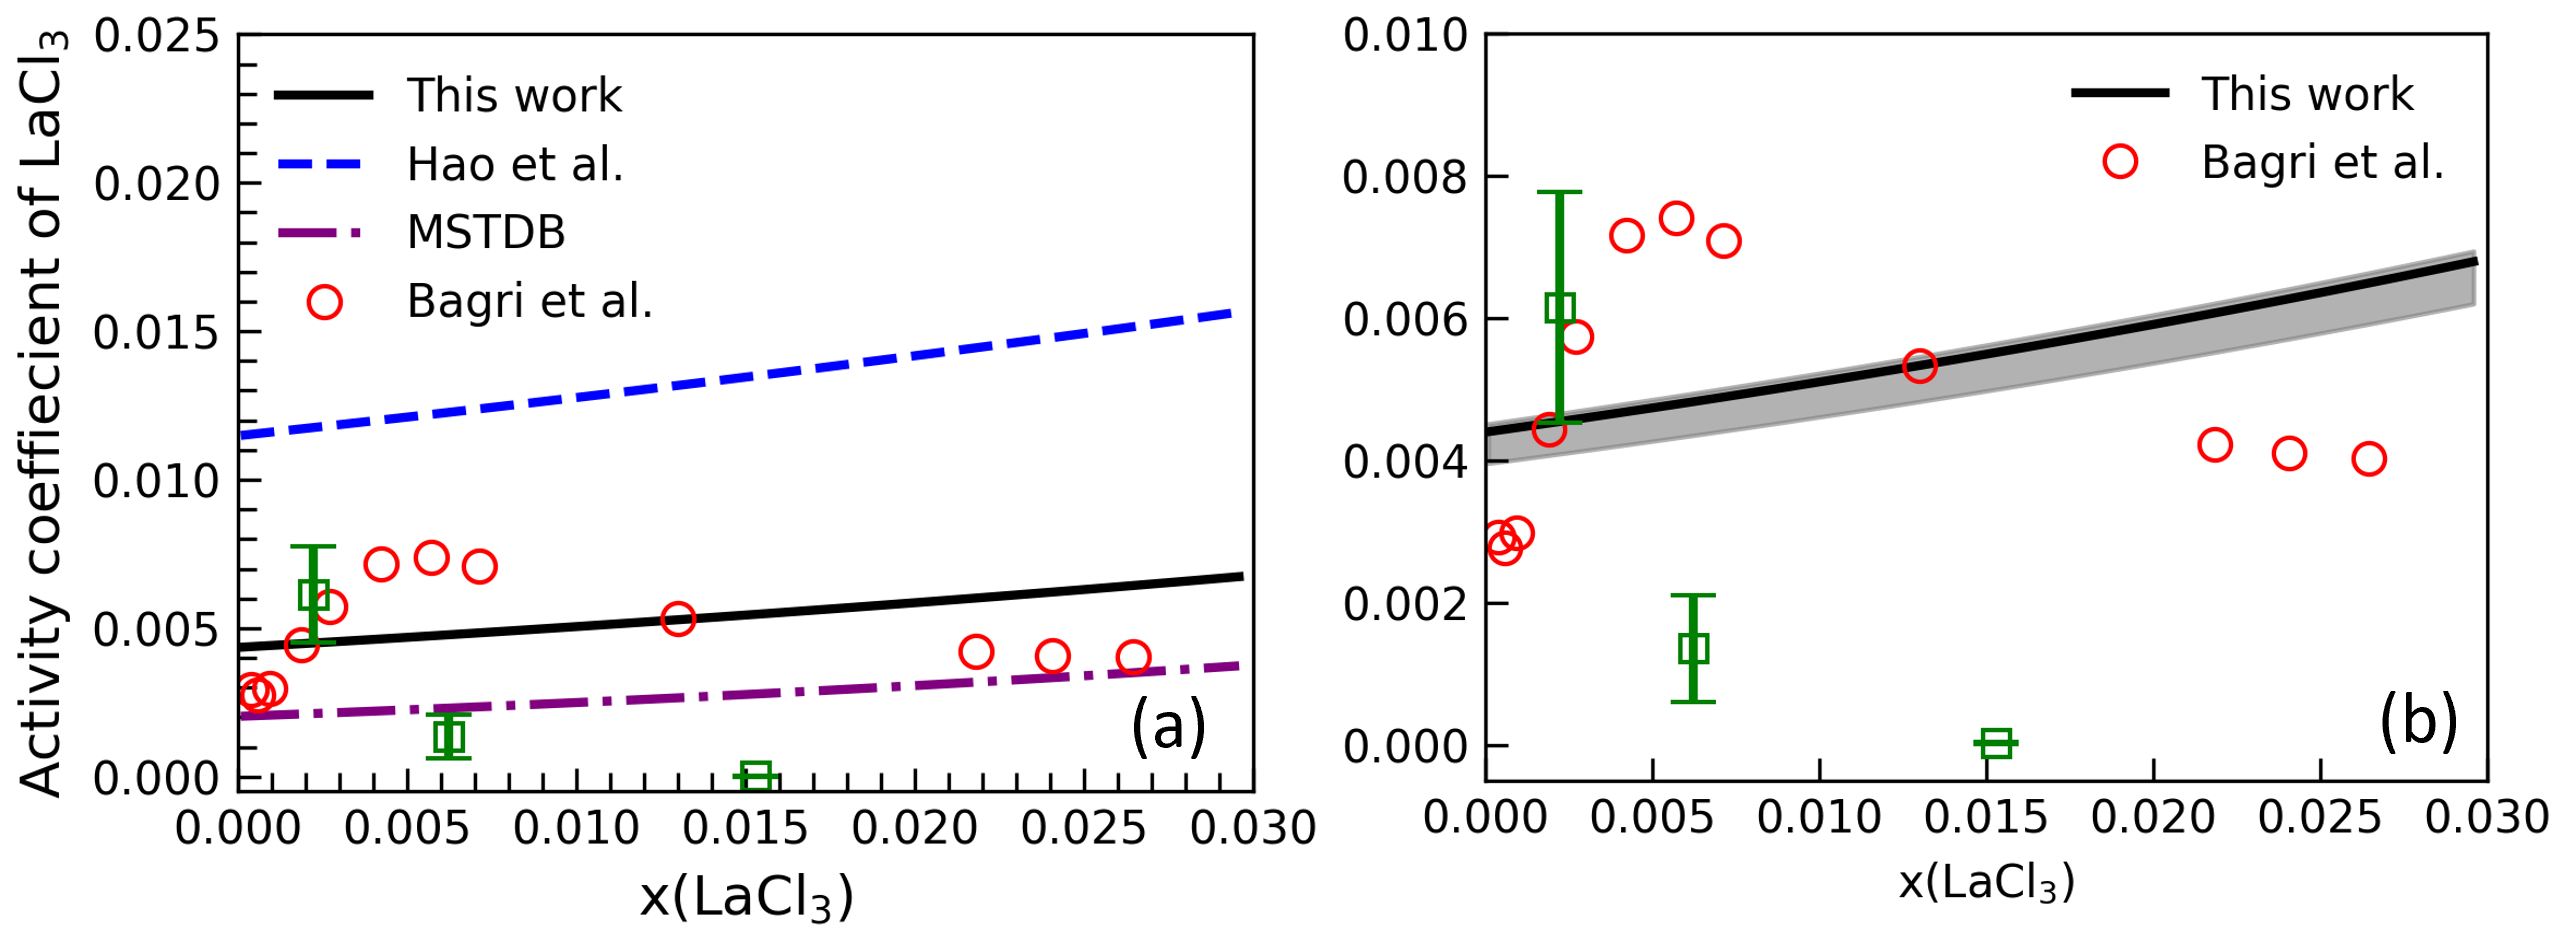
\includegraphics[width=1\linewidth]{moltensalts/Moltensalts-LaCl3-Gamma-Ternary-UQ.png}
    \caption{(a) Activity coefficients of LaCl$_3$ in KCl-LiCl eutectic at 773 K calculated from the present modeling in comparison with the modeling works from Hao et al. \cite{hao2024thermodynamic} (blue dash line) and MSTDB-TC \cite{ard2022development} (purple dash-dotted line), experimental measurements by Bagri et al. \cite{bagri2016determination} (red circles) and Samin et al. \cite{samin2016estimation} (green squares). (b) The uncertainty of the present modeling in predicting activity is shown in the grey region using a 95\% credible interval in predicting the activity values.}
    \label{ms:fig:lacl3ternaryGammaUQ}
\end{figure}

Thermodynamic properties predicted from the present CALPHAD modeling are compared with available experimental data. In addition, uncertainty quantification is performed to propagate parameter uncertainties into property predictions. Figure \ref{ms:fig:lacl3ternaryGammaUQ}(a) presents the values of the activity coefficient of LaCl$_3$ in the eutectic LiCl-KCl at 773 K, compared with the measurements by Bagri et al. \cite{bagri2016determination} and Samin et al. \cite{samin2016estimation}. The present modeling aligns more closely with the results by Bagri et al. \cite{bagri2016determination} since they provided a larger dataset over a broader composition range than those by Samin et al. \cite{samin2016estimation}. The model shows a good agreement in the low $x$(LaCl$_3$) region ($x$(LaCl$_3$) < 0.015) but slightly overestimates the activity coefficients when $x$(LaCl$_3$) increases to 0.02. The MAE of the present modeling, compared with values reported by Bagri et al. \cite{bagri2016determination}, is 0.0016. The present modeling represents a significant improvement over the previous work by Hao et al. \cite{hao2024thermodynamic}, which had an MAE of 0.0078 for predicting the activity coefficients. While MSTDB-TC \cite{ard2022development} shows a good agreement in the composition range of $x$(LaCl$_3$) from 0.022 to 0.027, it has a lower overall MAE of 0.0024 compared to the values reported by Bagri et al. \cite{bagri2016determination}. The present UQ values were performed using the last 10 MCMC iterations with 60 MCMC samples. The shadow region in Figure \ref{ms:fig:lacl3ternaryGammaUQ}(b) illustrates the uncertainties in predicting activity coefficients, with a 95\% credible interval (Bayesian credible intervals containing 95\% of the activity coefficients samples). This indicates that the present model has an uncertainty range of $-$10\% to +2\% in predicting the activity coefficient values.

\begin{figure} [H]
    \centering
    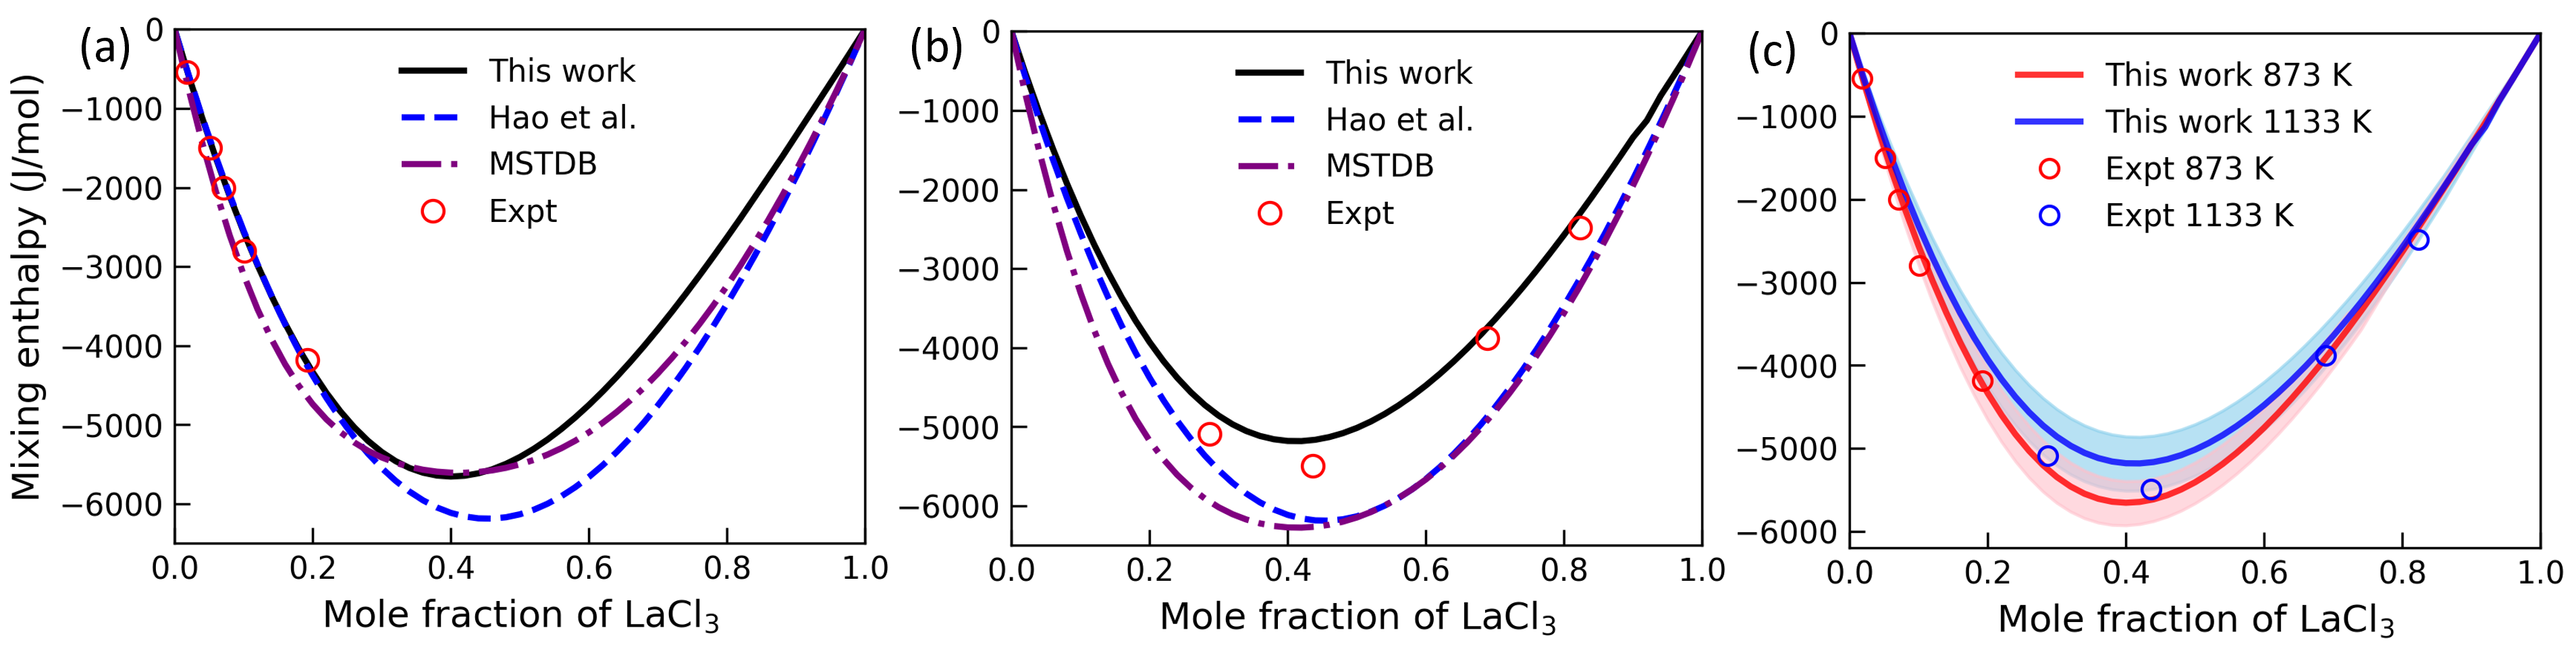
\includegraphics[width=1\linewidth]{moltensalts/Moltensalts-LaCl3-HMR-Ternary-UQ-models.png}
    \caption{Values of mixing enthalpy in LiCl-KCl-LaCl$_3$ at (a) 873 K and (b) 1133 K calculated from the present modeling compared with experimental measurements and the previous modeling works by Hao et al. \cite{hao2024thermodynamic} and MSTDB-TC \cite{ard2022development}. (c) The uncertainty of the present modeling in predicting mixing enthalpy is shown in the light red region (for 873 K) and the light blue region (for 1133 K) using a 95\% credible interval.}
    \label{ms:fig:lacl3ternaryHMRUQ}
\end{figure}


Figure \ref{ms:fig:lacl3ternaryHMRUQ} shows the mixing enthalpy calculations at 873 K and 1133 K from the present modeling, in comparison with experimental data and modeling results by Hao et al. \cite{hao2024thermodynamic} and MSTDB-TC \cite{ard2022development}. In Figure \ref{ms:fig:lacl3ternaryHMRUQ}(a), at 873 K, all these three modeling works closely match experimental measurements for $x$(LaCl$_3$) < 0.2. For example, at $x$(LaCl$_3$) = 0.1926, the present modeling predicts a mixing enthalpy of $-4231$ J/mol, which is 51 J/mol lower than the experimental value of $-4180$ J/mol. In comparison, Hao et al. \cite{hao2024thermodynamic} predicts $-4266$ J/mol and MSTDB-TC \cite{ard2022development} predicts $-4659$ J/mol, showing larger differences of 86 J/mol and 389 J/mol, respectively. The MAE of the present modeling in predicting mixing enthalpy at 873 K is 101 J/mol, compared to 120 J/mol for Hao et al. \cite{hao2024thermodynamic} and 312 J/mol for MSTDB-TC \cite{ard2022development}, highlighting the improved accuracy of the present modeling. Figure \ref{ms:fig:lacl3ternaryHMRUQ}(a) also shows different curve shapes in the LaCl$_3$-rich region predicted by three modeling works. The present modeling predicts a minimum energy similar to that by MSTDB-TC \cite{ard2022development} at around -5650 J/mol, whereas Hao et al. \cite{hao2024thermodynamic} predicts a value of $-6186$ J/mol, which is around 540 J/mol lower mixing enthalpy. Note that experiments investigations at 1133 K primarily focus on the LaCl$_3$-rich region.

Figure \ref{ms:fig:lacl3ternaryHMRUQ}(b) indicates that both Hao et al. \cite{hao2024thermodynamic} and MSTDB-TC \cite{ard2022development} predict lower values of mixing enthalpy compared to the present modeling and experiments. The present work improves the accuracy of mixing enthalpy predictions, reducing the MAE to 45.84 J/mol, compared to 159.75 J/mol by Hao et al. \cite{hao2024thermodynamic} and 183.30 J/mol by MSTDB-TC \cite{ard2022development}. Figure \ref{ms:fig:lacl3ternaryHMRUQ}(c) presents the uncertainty quantification of the present modeling in predicting mixing enthalpy, represented by the 95\% credible interval. At 873 K, the uncertainty range in predicting mixing enthalpy is around $-$5\% to +5\%. At 1133 K, the uncertainty range in predicting mixing enthalpy is around $-$6\% to +6\% with all existing experimental data falling within the lower boundary of the uncertainty region. This implies that the present modeling might underestimate the mixing enthalpy, particularly around $x$(LaCl$_3$) = 0.4. Further experiments or simulations in this composition range are recommended to enhance the accuracy of the present CALPHAD modeling. Figure \ref{ms:fig:lacl3quacf} shows the predicted fraction of each quadruplet in the liquid phase. The peak fractions of the LiLa/ClCl and LaK/ClCl quadruplets appear around $x$(LaCl$_3$) = 0.4, indicating the shorting range ordering (SRO) and it is consistent with the lowest mixing enthalpy around $x$(LaCl$_3$) = 0.4. 

\begin{figure} [H]
    \centering
    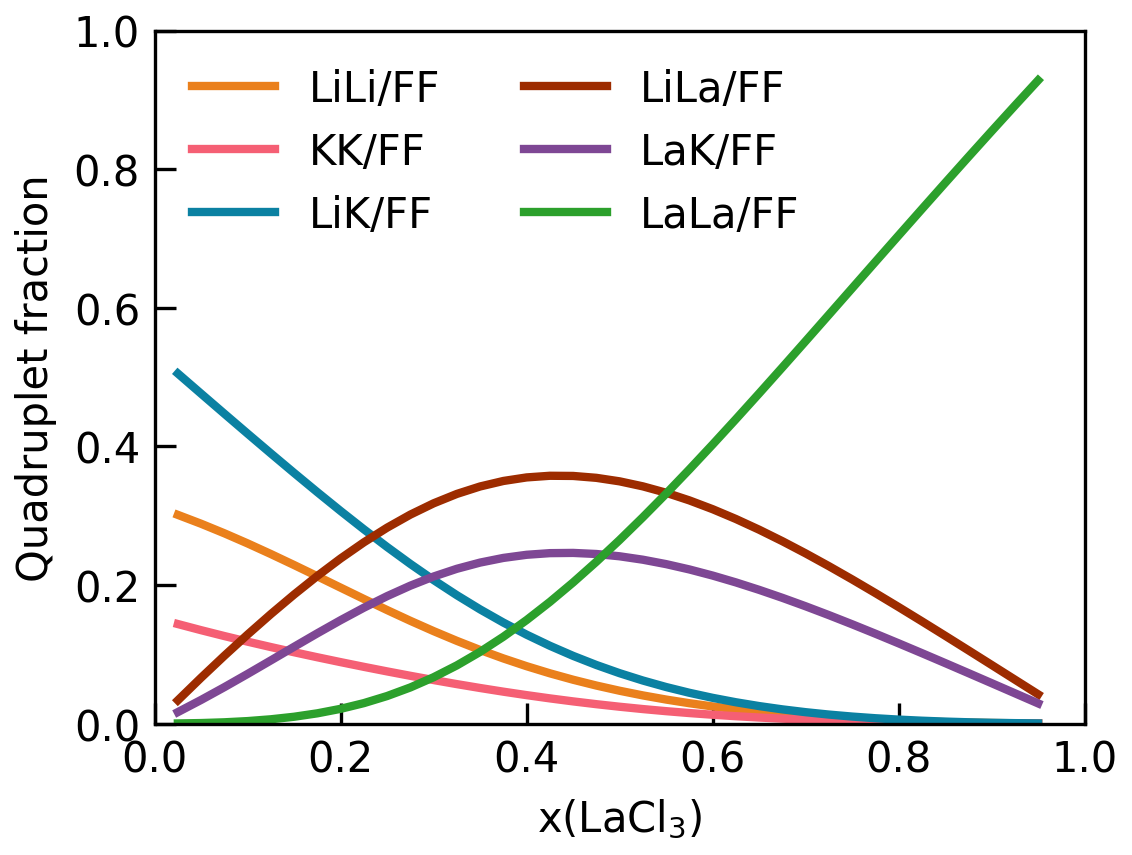
\includegraphics[width=0.6\linewidth]{moltensalts/Moltensalts-LaCl3-QuadFrac-LaCl3-LiCl-KCl.png}
    \caption{Precited quadruplet fractions in the LiCl-KCl-LaCl$_3$ liquid at 1133 K according to the present CALPHAD modeling using MQMQA.}
    \label{ms:fig:lacl3quacf}
\end{figure}

\begin{figure} [H]
    \centering
    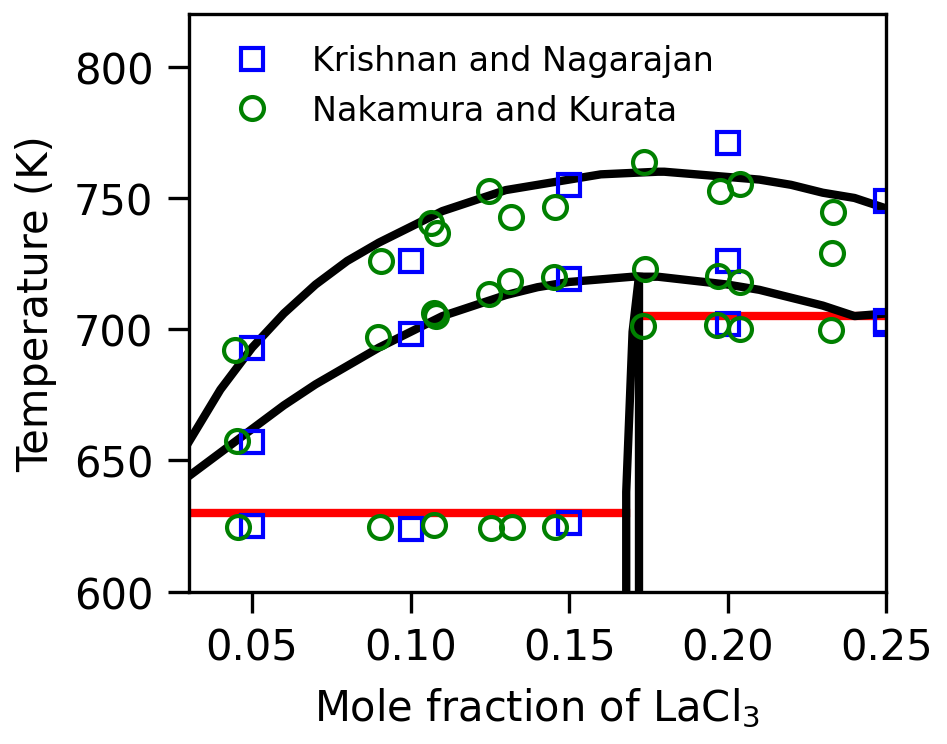
\includegraphics[width=0.6\linewidth]{moltensalts/Moltensalts-Isopleth-LaCl3-LiCl-KCl.png}
    \caption{Partial isopleth between the eutectic KCl-LiCl and LaCl$_3$ calculated from the present modeling work in comparison with experimental measurements by Venkata Krishnan et al. (blue squares) \cite{venkata2006pseudo} and Nakamura and Kurata (green circles) \cite{nakamura1997thermal}.}
    \label{ms:fig:lacl3ternaryisopleth}
\end{figure}

Figure \ref{ms:fig:lacl3ternaryisopleth} shows the partial isopleth between the eutectic KCl-LiCl and LaCl$_3$ calculated from the present CALPHAD modeling compared with experimental measurements \cite{nakamura1997thermal, venkata2006pseudo}, demonstrating a close match of liquidus and solidus lines. For the eutectic reaction Liquid$\leftrightarrow$KCl+LiCl\\+K$_2$LaCl$_5$, the present modeling predicts a eutectic temperature of 630 K, which is 5 K higher than the 625 K reported by Nakamura et al. \cite{nakamura1997thermal} and Venkata Krishnan et al. \cite{venkata2006pseudo}. Similarly, for the reaction Liquid$\leftrightarrow$LiCl+K$_2$LaCl$_5$+ K$_3$La$_5$Cl$_{18}$, the present modeling predicts the eutectic temperature at 705 K, which is 3 K higher than the reported 702 K by Nakamura et al. \cite{nakamura1997thermal} and Venkata Krishnan et al. \cite{venkata2006pseudo}. Overall, the present modeling of LiCl-KCl-LaCl$_3$ demonstrates a good agreement with experimental data \cite{bagri2016determination,samin2016estimation,nakamura1997thermal, venkata2006pseudo} regarding phase boundary properties. 

\section{Summary} \label{moltensalts:sec:Summary}
This chapter investigates the thermodynamic properties of compounds and liquids in the (LiF, NaF, KF, CrF$_2$)-CrF$_3$ systems by utilizing CALPHAD modeling with inputs from the DFT-based first-principles, phonon, and AIMD calculations. Thermodynamic properties, including enthalpy, entropy, and heat capacity of the binary (endmember) compounds LiF, NaF, KF, CrF$_3$, and CrF$_2$ as a function of temperature, have been predicted by DFT-based phonon calculations, agreeing with available experimental data in the literature and validating the reliability of the present methodology. They enabled the remodeling of the (LiF, NaF, KF, CrF$_2$)-CrF$_3$ systems with more accurate inputs. The MQMQA is employed to describe the liquid phase, providing valuable insights into the complex nature of molten salts such as the short-range ordering and neighboring of cations. Phase equilibria from the present CALPHAD modeling match better with experimental data in comparison with previous modeling work in the literature. The present thermodynamic data, including equilibrium volumes, bulk moduli, enthalpies, entropies, and heat capacities of compounds in the (LiF, NaF, KF, CrF$_2$)-CrF$_3$ system can be used to facilitate the development of advanced molten salt reactors.

In addition, this chapter demonstrates an application of Bayesian model selection to identify the optimal model for describing atomic environments in molten salts, focusing on the KCl-LaCl$_3$ system. Four candidate models are considered, which are the associate model, the two-sublattice ionic model, and two MQMQA models with different coordination numbers. By estimating the marginal likelihoods of each model from MCMC optimization and calculating Bayes factors to compare models, one of the MQMQA models is suggested as the most favorable one to describe the KCl-LaCl$_3$ system based on available input data. DFT-based calculations provide important thermodynamic properties for compounds in KCl-LaCl$_3$, including equilibrium volumes, bulk moduli, enthalpies, entropies, and heat capacities. Furthermore, the ternary LiCl-KCl-LaCl$_3$ system is modeled, demonstrating a better agreement with experimental data compared to the previous CALPHAD modeling works in the literature. The uncertainty quantification and propagation show that the present modeling provides reliable predictions of activity and mixing enthalpy when compared with experimental data. The present work indicates that the Bayesian model selection approach facilitates a more rational comparison among different liquid models, enhancing the accuracy of thermodynamic predictions in molten salts.